% =====================================================================================================
%  Chapter 24 (key `front`) -- 其他前沿严格结果
%  Writer W27.  Binding inputs: writing/LEAD_DECISIONS.md, spec_v2/WRITER_SPEC_v2.md (v2.3.1),
%  spec_v2/FINAL_OUTLINE_v2.md (Ch24 section and Part VII annexes), spec_v2/VERIFIED_FORMULAS_v2.md (VF-FRO-*).
%  Re-derivation scripts and logs: writing/work/W27/s_*.py, s_*.log.
%  Key clash: this chapter never defines tab:front-notation* (owned by the front matter).
% =====================================================================================================
\chapter{其他前沿严格结果}\label{ch:front}

本章逐条记录约 2010 年以来，在本书前六部分所依赖的基础之上取得的严格结果、全阶论证、显式验证与反例（LaMET 与 Yizhuang Liu 的研究纲领见前两章），并给出每一条的精确适用范围与分级。本章自己完整证明的只有两条数学引理（\cref{lem:front-min-norm,lem:front-jantzen}）、两条条件定理（\cref{cor:front-coleman-norton,prop:front-commuting}，\tagR，$R_{\mathrm{cond}}$，内容等级分别为 [A] 与 [C]）、Yukawa 模型中单圈 $\MSbar$ 分布可以为负的计算（\cref{prop:front-msbar-negative}(a)，\tagR，$R_{\mathrm{PT}}$），以及若干反例与级数恒等式；其余条目按文献所能支持的程度精确转述并分级：二十七条全阶论证 [A]、十一条部分结果 [P]、六条猜想 [C]、七条已知不成立的陈述 [V]。

\begin{tcolorbox}[enhanced,breakable,title=本章证明了什么／没有证明什么,fonttitle=\bfseries,
  colback=gray!3!white,colframe=gray!55!black,boxrule=0.6pt,arc=2pt,
  left=5pt,right=5pt,top=3pt,bottom=3pt,before skip=6pt,after skip=6pt]
\textbf{证明了：}\cref{lem:front-min-norm,lem:front-jantzen}（数学；后者在其局部假设 (J1)--(J4) 之下）；\cref{prop:front-lp-facets,prop:front-onshell-facets}（\tagR，$R_{\mathrm{PT}}$，证明见所引文献）；\cref{cor:front-coleman-norton}（\tagR，$R_{\mathrm{cond}}$，前提\cref{thm:front-collins-pinch}）；\cref{prop:front-commuting}（\tagR，$R_{\mathrm{cond}}$，前提\cref{asm:front-mor-complete}）；\cref{prop:front-msbar-negative}(a)（单圈 Yukawa 模型，\tagR，$R_{\mathrm{PT}}$）。已知不成立（\tagV）：\cref{prop:front-anomalous,prop:front-landau-not-singular,prop:front-hidden-regions,prop:front-jettiness-cvl,prop:front-msbar-negative,prop:front-regge-pole,prop:front-ew-violation}。\par
\textbf{给出全阶论证：}\cref{thm:front-collins-pinch}（\tagA，证明仅见于预印本）；\cref{prop:front-ir-forest,prop:front-coordinate-space,prop:front-glauber-bfkl,prop:front-syz,prop:front-heavy-fsi,prop:front-sll-all-orders,prop:front-sll-closed-form,thm:front-hgg,prop:front-ggh,prop:front-nlp-ll,prop:front-nlp-dis,prop:front-tmd-nlp-operator,prop:front-sidis-nlp,prop:front-brst-bilocal,prop:front-nlo-bk,prop:front-regge,prop:front-smallx-tmd,prop:front-smallx-helicity,prop:front-dps-scheme,prop:front-rapidity-renorm,prop:front-ngl,prop:front-jet-substructure,prop:front-lightray-ope,thm:front-luxqed,prop:front-lepton-pdf,prop:front-ew-pdf}（\tagA；\cref{thm:front-hgg,prop:front-ggh,prop:front-nlp-ll,prop:front-nlp-dis,prop:front-sidis-nlp}的瓶颈为\cref{asm:front-scet-modes}，\cref{prop:front-nlp-dis}的论证仅见于预印本）。部分结果（\tagP，有限阶、模型或子类）：\cref{prop:front-local-ir,prop:front-ope-scalar,prop:front-ope-ym,prop:front-flow-renorm,prop:front-restoration,prop:front-nlp-threshold,prop:front-nlp-tmd-oneloop,prop:front-positivity-large-scale,prop:front-bk-collinear,prop:front-dpd-evolution,prop:front-nrqcd-ir}。\par
\textbf{没有证明：}\cref{conj:front-ope-convergence,conj:front-mor-minkowski,conj:front-mpi-violation,conj:front-nlp-beyond-ll,conj:front-glauber-nlp,conj:front-brst-multilocal}（\tagC）；区域集合的完备性\cref{asm:front-mor-complete}（\tagC，\cref{conj:front-mor-minkowski}的前提形式）；本章没有任何一条陈述控制 QCD 中因子化的非微扰有效性。
\end{tcolorbox}

% -----------------------------------------------------------------------------------------------------
\section{引言：范围、重叠规则与阅读深度}\label{sec:front-intro}

本书第二至第六部分的证明建立在少数几条基础性陈述之上：钳夹面的位置及其 Landau 判据与 Coleman--Norton 图像（\cref{sec:ir-landau}），OPE 成立的意义（\cref{thm:dis-ope}、\cref{thm:power-ope-convergence}），区域方法与 SCET 模式表的地位（\cref{sec:ir-regions}），Glauber 区在单举 Drell--Yan 中相消而在别处未必相消（\cref{thm:dy-factorization}，\cref{sec:break-mpi}），非全局可观测量的对数结构（\cref{sec:jets-ngl}），以及幂次修正的组织（\cref{prop:power-nlp-endpoint}）。本章回答：自 2010 年前后以来，这些基础中哪些发生了变化，朝哪个方向变化。变化分三类：把只有启发式论证的结论变成有书面证明的定理（最突出的是 Collins 的物理区钳夹判据，\cref{thm:front-collins-pinch}；证明只见于预印本，本书仍记为 [A]）；证伪被普遍使用的一般陈述（\cref{prop:front-hidden-regions,prop:front-msbar-negative,prop:front-jettiness-cvl,prop:front-regge-pole}）；以及原有框架内的精细化（超领头对数的全阶重求和、次领头幂次的端点因子化、无重复计数的双部分子散射、由结构函数确定光子分布等）。

\paragraph{重叠规则与阅读深度。}前面各章已陈述的核心结论在此从不重述；本章只给出前沿细化（标签前缀 \texttt{front}），并在首次出现时注明所引核心陈述的等级（\cref{tab:front-map}）。读过全文的文献，我们给出定理与公式的位置；只读到摘要层次的文献，转述注明“据该文摘要”，不作超出摘要的断言。截至 2026 年 10 月仍只有 arXiv 版本的文献是\cite{Collins:2020euz,Frob:2016mzv,Guida:2011np,Beneke:2026miy,Gamberg:2022lju,Bodwin:2025zzi,Anastasiou:2025cvy,Anastasiou:2026kpm,Anastasiou:2026jta,Becher:2026zon,Becher:2026iim}（预印本），依赖它们的「地位与缺口」段都重申这一点。不同研究组之间的分歧，我们并列给出各自结论的确切适用范围，不作裁决。

\paragraph{全局性保留与约定。}本章所有“严格”结果都是微扰论（在每一固定圈数）或模型中的陈述；唯一的非微扰正面结论是共形场论中的光线 OPE（\cref{prop:front-lightray-ope}(b)），其余非微扰陈述都是反例。没有任何一条结论控制 QCD 中因子化的非微扰有效性，后者仍由第一章的全局假设（如\cref{asm:intro-bridge}）承担。记号沿用全书约定，三处例外在用到时说明：\cref{sec:front-landau}沿用 Collins 的积分记号（分母 $A_j$、梯度 $D_j$、二阶导数 $E_j$）；\cref{sec:front-glauber}与\cref{sec:front-nlp}所引 SCET 算符采用\cref{def:scet-modes}的约定；喷注文献中的多 Wilson 线软函数 $S_i=\mathbf P\exp(\ii g_s\int_0^\infty\dd s\,n_i\cdot A^a_s\mathbf T^a_i)$\cite{Becher:2016mmh}的耦合符号与本书相反（换算到本书约定：$g\to-g$），本章只引用由它们得到的、对 $g$ 为偶的结果。

\begin{table}[htbp]
\centering
\caption{前沿主题、核心陈述与本章的细化。中间一列是前面各章（或附录）中的核心陈述及其等级，右列是本章对应的细化条目。}\label{tab:front-map}
\small
\renewcommand{\arraystretch}{1.1}
\begin{tabularx}{\textwidth}{@{}p{2.4cm}>{\raggedright\arraybackslash}X>{\raggedright\arraybackslash}X@{}}
\toprule
主题（节） & 核心陈述（等级） & 本章的细化 \\
\midrule
Landau 判据、Coleman--Norton（\cref{sec:front-landau}） & \cref{thm:ir-landau-momentum}（[R, $R_{\mathrm{PT}}$]）、\cref{rem:ir-landau-status}（[A]）、\cref{prop:ir-coleman-norton}（[R, $R_{\mathrm{PT}}$]）；\cref{lem:appD-gordan}（数学） & \cref{def:front-trap,lem:front-min-norm,thm:front-collins-pinch,cor:front-coleman-norton,prop:front-anomalous,prop:front-landau-not-singular,prop:front-ir-forest,prop:front-coordinate-space,prop:front-local-ir} \\
OPE（\cref{sec:front-ope}） & \cref{thm:dis-ope}（[A]）、\cref{thm:power-ope-convergence}（[R, $R_{\mathrm{PT}}$]） & \cref{prop:front-ope-scalar,prop:front-ope-ym,prop:front-flow-renorm,conj:front-ope-convergence} \\
区域方法（\cref{sec:front-regions}） & \cref{def:ir-regions}、\cref{thm:ir-regions-euclid}（[R, $R_{\mathrm{PT}}$]）、\cref{prop:ir-regions-minkowski}（[P]）；\cref{def:scet-zero-bin} & \cref{lem:front-jantzen,def:front-facets,prop:front-lp-facets,prop:front-onshell-facets,prop:front-commuting,prop:front-hidden-regions,conj:front-mor-minkowski} \\
Glauber（\cref{sec:front-glauber}） & \cref{prop:scet-glauber-operators}（[A]）、\cref{thm:dy-factorization}（[A]）、\cref{prop:break-spacelike,prop:break-fss,prop:break-jet-veto}（[V]）、\cref{prop:break-mass-singularity}（[C]） & \cref{prop:front-glauber-bfkl,prop:front-syz,conj:front-mpi-violation,prop:front-heavy-fsi} \\
超领头对数（\cref{sec:front-sll}） & \cref{prop:jets-sll}（[P]）、\cref{thm:jets-ngl-factorization}（[A]） & \cref{prop:front-sll-all-orders,prop:front-sll-closed-form,prop:front-restoration,prop:front-jettiness-cvl} \\
次领头幂次（\cref{sec:front-nlp}） & \cref{prop:thr-nlp}（[P]）、\cref{prop:power-nlp-endpoint}（[P]） & \cref{thm:front-hgg,prop:front-ggh,prop:front-nlp-threshold,prop:front-nlp-ll,prop:front-nlp-dis,conj:front-nlp-beyond-ll} \\
次领头幂次 TMD（\cref{sec:front-nlp-tmd}） & \cref{thm:tmd-factorization}（[A]） & \cref{conj:front-glauber-nlp,prop:front-tmd-nlp-operator,prop:front-sidis-nlp,prop:front-nlp-tmd-oneloop} \\
正定性（\cref{sec:front-positivity}） & \cref{conj:pdf-positivity}（[C]） & \cref{prop:front-msbar-negative,prop:front-positivity-large-scale} \\
BRST 分类（\cref{sec:front-brst}） & \cref{prop:appJ-local-operators}（[R, $R_{\mathrm{PT}}$]）、\cref{rem:appJ-nonlocal}、\cref{prop:appL-renormalized}（[R, $R_{\mathrm{PT}}$]） & \cref{prop:front-brst-bilocal,conj:front-brst-multilocal} \\
小 $x$（\cref{sec:front-smallx}） & \cref{thm:smallx-bfkl,thm:smallx-bk}（[A]） & \cref{prop:front-nlo-bk,prop:front-bk-collinear,prop:front-regge,prop:front-regge-pole,prop:front-smallx-tmd,prop:front-smallx-helicity} \\
双部分子散射（\cref{sec:front-dps}） & \cref{def:break-dpdf}、\cref{thm:break-double-dy}（[A]）、\cref{conj:break-dps-coloured}（[C]） & \cref{prop:front-dps-scheme,prop:front-rapidity-renorm,prop:front-dpd-evolution} \\
喷注与非全局对数（\cref{sec:front-jets}） & \cref{thm:jets-ngl-factorization,thm:jets-bms}（[A]）、\cref{prop:jets-ngl-beyond}（[P]） & \cref{prop:front-ngl,prop:front-jet-substructure,prop:front-lightray-ope} \\
重夸克偶素（\cref{sec:front-quarkonium}） & \cref{conj:heavy-nrqcd-production}（[C]）、\cref{prop:heavy-quarkonium-fragmentation}（[A]） & \cref{prop:front-nrqcd-ir} \\
QED 与电弱（\cref{sec:front-qed}） & \cref{prop:ir-bn-failure}（[V]）、\cref{prop:coll-luxqed}（[A]） & \cref{thm:front-luxqed,prop:front-lepton-pdf,prop:front-ew-pdf,prop:front-ew-violation} \\
\bottomrule
\end{tabularx}
\end{table}

% -----------------------------------------------------------------------------------------------------
\section{物理区钳夹判据、Gordan 二择一与 Coleman--Norton 图像}\label{sec:front-landau}

第四章证明了 Landau 条件是钳夹的必要条件（\cref{thm:ir-landau-momentum}，[R, $R_{\mathrm{PT}}$]），而把充分性与局部形变的整体拼接记为全阶论证（\cref{rem:ir-landau-status}，[A]）；Collins 在 2011 年写道，文献中没有“Landau 方程对钳夹奇异面既必要又充分”的公开、显式而完整的证明\cite[第~5.4.3~节，第~110~页]{Collins2011}。本节记录 Collins 2020 年的工作\cite{Collins:2020euz}（预印本）补上了什么，以及其中可以化为经典凸几何的一半。

\begin{definition}[围道变形、钳夹、Landau 点与好方向]\label{def:front-trap}
考虑积分
\begin{equation}\label{eq:front-collins-integral}
I(z)=\lim_{\epsilon\to0^+}\int_{\Gamma_0}\dd^dw\,\frac{B(w;z)}{\prod_{j=1}^N\bigl[A_j(w;z)+\ii\epsilon\bigr]^{n_j}},\qquad n_j\notin\{0,-1,-2,\dots\},
\end{equation}
外参数 $z$ 为实数，$\Gamma_0$ 为全体实的 $w$，$A_j$、$B$ 解析且 $A_j$ 对实宗量取实值（$\epsilon$ 是 $\ii\epsilon$ 处方的参数）；Feynman 图是 $w=$ 圈动量、$A_j=k_j^2-m_j^2$（允许 $m_j=0$）的情形，也包括 Wilson 线的线性分母 $n\cdot k_j$ 与近似分母。\emph{围道形变} $w=w_R+\ii\tau v(w_R)$，$0\le\tau\le1$，$v$ 实、连续、分段可微、在边界上为零。形变在 $w_S$ 附近\emph{容许}，指存在 $\epsilon_0>0$，使在 $w_S$ 的某邻域内、$0\le\tau\le1$、$0<\epsilon\le\epsilon_0$ 时所有 $A_j+\ii\epsilon\ne0$；容许形变\emph{避开} $w_S$ 处的奇点，指该非零性在 $\epsilon=0$、$0<\tau\le1$ 时仍成立；没有容许形变避开 $w_S$ 处的奇点时，称积分在 $w_S$ \emph{被钳住}（trapped，pinched）。对在 $w_S$ 为零的分母 $\{A_j\}_{j\in J}$，记对偶向量 $D_j=\partial A_j(w_S)$（与时空维数无关）。不全为零的 $\lambda_j\ge0$ 若满足 $\sum_{j\in J}\lambda_jD_j=0$，称为 \emph{Landau 点}（正性 $\lambda_j\ge0$ 是物理区钳夹区别于一般复奇点之处）；对一切 $j\in J$ 有 $D_j\cdot v>0$ 的 $v$ 称为\emph{好方向}；避开了奇点、却对某个 $j\in J$ 有 $v(w_S)\cdot D_j=0$ 的容许形变称为\emph{反常形变}。
% VF-FRO-2
% uses: none
\end{definition}

以上取自\cite[第~II~节，定义~1--7、15]{Collins:2020euz}。第四章的钳夹面（\cref{def:ir-pinch-surface}）正是 Feynman 积分被钳住的点之集；注意\cref{thm:ir-landau-momentum}的记号与此不同。

\begin{lemma}[Gordan 二择一的构造性形式：最小范数方向]\label{lem:front-min-norm}
设 $D_1,\dots,D_N$ 是有限维实向量空间 $V$ 上的对偶向量，在 $V^*\simeq V$ 上取定内积，$K=\mathrm{conv}\{D_1,\dots,D_N\}$。(i) 存在 Landau 点当且仅当 $0\in K$；(ii) 若 $0\notin K$，则 $K$ 中范数最小的点 $w$ 唯一，且对一切 $j$ 有 $D_j\cdot w\ge|w|^2>0$，即 $w$ 是带余量 $|w|^2$ 的好方向；(iii) Landau 点与好方向不能同时存在。
% VF-FRO-1
% uses: none
\end{lemma}

\begin{proof}
(i) 凸组合的权重 $\mu_j$（$\sum_j\mu_j=1$）就是 Landau 点；反之 Landau 点除以 $\sum_j\lambda_j>0$ 给出 $0\in K$。(ii) $K$ 非空紧凸，$|u|^2$ 严格凸，故 $w$ 存在唯一且 $w\ne0$。对 $u\in K$、$t\in(0,1]$，$0\le|w+t(u-w)|^2-|w|^2=2t\langle w,u-w\rangle+t^2|u-w|^2$，除以 $t$ 并令 $t\to0^+$ 得 $\langle w,u\rangle\ge|w|^2$，取 $u=D_j$。(iii) 否则 $0=\sum_j\lambda_jD_j\cdot v>0$。
\end{proof}

(i)--(iii) 合起来是 Gordan 择一定理（\cref{lem:appD-gordan}）的构造性证明。
% Numerical check (writer): writing/work/W27/s_landau.py, 300 random instances, margin deficit < 2e-15;
% frontier check OTHERS s1(a): 400 instances (226 type I, 174 type II).

\begin{remark}[Collins 的几何定理即 Gordan 二择一]\label{rem:front-gordan-collins}
Collins 证明中纯几何的一半——好方向存在当且仅当不存在 Landau 点\cite[定理~3]{Collins:2020euz}——原文用约十二页（第~V--VII~节）证明，作者在脚注~6 中说尚未在凸几何文献中找到所需的结果。它正是 Gordan 1873 年的择一定理\cite{Gordan1873}（对实矩阵 $D$，“存在 $v$ 使 $Dv>0$”与“存在非零 $\lambda\ge0$ 使 $D^{\mathsf T}\lambda=0$”恰有一个成立）；最小范数方向可直接用于数值围道形变（这类方法见\cite{Gong:2008ww,Becker:2012nk}）。据我们截至 2026 年 10 月的文献检索（INSPIRE 全文检索与\cite{Collins:2020euz}的全部施引文献；早于 arXiv 的文献未作全文检索），尚未见在 Landau 分析的文献中引用 Gordan 定理。这一等同是初等的；Collins 证明中分析的那一半（排除反常形变）不受影响。
\end{remark}

\begin{example}[二维中的两种情形]\label{ex:front-gordan-2d}
(a) $D_1=(2,0)$、$D_2=(1,2)$：$|(1-t)D_1+tD_2|^2=(2-t)^2+4t^2$ 在 $t=\frac25$ 最小，$w=(\frac85,\frac45)$，$|w|^2=\frac{16}5=D_1\cdot w=D_2\cdot w$；好方向锥是方向角介于 $-26.57^\circ$ 与 $90^\circ$ 之间的开锥，$w$（$26.57^\circ$）在其中；\cref{fig:front-gordan}(a) 另画的 $D_3=(2.6,1.6)$ 有 $D_3\cdot w=5.44>|w|^2$，最小点不变。(b) 加入 $D_3=(-1,-1)$ 后 $1\cdot D_1+2\cdot D_2+4\cdot D_3=0$，没有好方向（\cref{fig:front-gordan}(b)）。
\uses{lem:front-min-norm}
\end{example}

%%% BEGIN fig:front-gordan
\begin{figure}[htbp]
\centering
% Data: (a) D1=(2,0), D2=(1,2) (ex:front-gordan-2d), D3=(2.6,1.6) on the far side of the
% line D1D2; min-norm point of conv{D_j}: w=(8/5,4/5), |w|^2=16/5=D1.w=D2.w, D3.w=5.44;
% good cone {v: D_j.v>0} = directions between -26.57 deg (perp. to D2) and 90 deg (perp. to D1).
% (b) D3=(-1,-1): 1*D1+2*D2+4*D3=0 (closed polygon drawn at scale 0.4).
\begin{tikzpicture}[fd,
  fe vec/.style={draw,line width=0.9pt,-{Stealth[length=6pt,width=4.6pt]}},
  fe hull/.style={draw=gray!65,fill=gray!22,line width=0.6pt,line join=round},
  fe cone/.style={fill=green!9,draw=none},
  fe ray/.style={draw=green!45!black,line width=0.6pt,dash pattern=on 3pt off 2pt},
  fe wpt/.style={circle,fill=red!65!black,draw=none,inner sep=0pt,minimum size=4.6pt},
  fe lam/.style={draw=blue!60!black,line width=0.9pt,-{Stealth[length=6pt,width=4.6pt]}},
  fe lab/.style={font=\footnotesize}]
  % ======================= (a) good direction =======================
  \begin{scope}
    \fill[fe cone] (0,0) -- (-26.565:2.95) arc[start angle=-26.565,end angle=90,radius=2.95] -- cycle;
    \draw[fe ray] (0,0) -- (90:2.95);
    \draw[fe ray] (0,0) -- (-26.565:2.95);
    \draw[lcaxis,gray!55] (-1.15,0) -- (3.35,0);
    \draw[lcaxis,gray!55] (0,-1.75) -- (0,3.3);
    % supporting line v.w = |w|^2 through D1, D2
    \draw[gray!60!black,densely dotted,line width=0.6pt] ($(2,0)!-0.45!(1,2)$) -- ($(2,0)!1.32!(1,2)$);
    \draw[fe hull] (2,0) -- (1,2) -- (2.6,1.6) -- cycle;
    \draw[fe vec] (0,0) -- (2,0);
    \draw[fe vec] (0,0) -- (1,2);
    \draw[fe vec] (0,0) -- (2.6,1.6);
    \draw[red!65!black,line width=0.7pt,dash pattern=on 2.5pt off 1.8pt] (0,0) -- (1.6,0.8);
    % right-angle mark at w on the D1 side (face direction (1,-2)/sqrt5, normal (2,1)/sqrt5),
    % away from the arrow D3 which passes just above w
    \draw[red!65!black,line width=0.5pt] ($(1.6,0.8)+(0.0894,-0.1789)$) -- ++(-0.1789,-0.0894) -- ++(-0.0894,0.1789);
    \node[fe wpt] at (1.6,0.8) {};
    \node[anchor=north east,inner sep=1.5pt] at (2.02,-0.03) {$D_1$};
    \node[anchor=east,inner sep=2pt] at (0.98,2.05) {$D_2$};
    \node[anchor=west,inner sep=2pt] at (2.62,1.62) {$D_3$};
    \node[inner sep=1pt,text=red!60!black] at (1.27,0.42) {$w$};
    \node[fill=white,fill opacity=0.85,text opacity=1,inner sep=1pt] at (0,0) {};
    \node[anchor=north east,inner sep=1.5pt] at (0,0) {$0$};
    \node[fe lab,text=green!35!black,anchor=south,align=center] at (1.5,2.82) {好方向锥 $\{v:D_j\cdot v>0\}$};
    \node[fe lab,text=gray!40!black,anchor=north west] at (2.38,-0.62) {$v\cdot w=|w|^2$};
    \node at (1.05,-2.25) {(a)\ $D_j\cdot w\ge|w|^2$：好方向};
  \end{scope}
  % ======================= (b) Landau point =======================
  \begin{scope}[xshift=7.1cm]
    \draw[lcaxis,gray!55] (-1.75,0) -- (2.75,0);
    \draw[lcaxis,gray!55] (0,-1.75) -- (0,3.3);
    \draw[fe hull] (2,0) -- (1,2) -- (-1,-1) -- cycle;
    \draw[fe vec] (0,0) -- (2,0);
    \draw[fe vec] (0,0) -- (1,2);
    \draw[fe vec] (0,0) -- (-1,-1);
    \node[circle,fill=black,draw=none,inner sep=0pt,minimum size=3.6pt] at (0,0) {};
    \node[anchor=north west,inner sep=1.5pt] at (1.98,-0.03) {$D_1$};
    \node[anchor=east,inner sep=2pt] at (0.98,2.05) {$D_2$};
    \node[anchor=north east,inner sep=1.5pt] at (-1,-1) {$D_3$};
    \node[anchor=south east,inner sep=1.5pt] at (-0.05,0.05) {$0$};
    % closed polygon of the weighted vectors (scale 0.4)
    \begin{scope}[shift={(2.85,0.55)},scale=0.4]
      \draw[fe lam] (0,0) -- (2,0);
      \draw[fe lam] (2,0) -- (4,4);
      \draw[fe lam] (4,4) -- (0,0);
      \node[fe lab,anchor=north,inner sep=2pt] at (1,0) {$\lambda_1D_1$};
      \node[fe lab,anchor=west,inner sep=2pt] at (3,2) {$\lambda_2D_2$};
      \node[fe lab,anchor=south east,inner sep=1pt] at (2,2.05) {$\lambda_3D_3$};
    \end{scope}
    \node[fe lab,align=center,anchor=north] at (3.6,-0.35) {$\lambda=(1,2,4)$\\[1pt]$\sum_j\lambda_jD_j=0$};
    \node at (1.25,-2.25) {(b)\ Landau 点：无好方向};
  \end{scope}
\end{tikzpicture}
\caption{Gordan 二择一定理（1873）\cite{Gordan1873}：对有限个对偶矢量 $D_j$，要么存在好方向 $v$（$D_j\cdot v>0$，可取凸包中范数最小的点 $w$，并有 $D_j\cdot w\ge|w|^2$），要么存在 Landau 点（$\lambda_j\ge0$ 不全为零、$\sum_j\lambda_jD_j=0$），二者恰有其一。
(a)~$D_1=(2,0)$、$D_2=(1,2)$ 与 $D_3$ 的凸包（灰）不含原点，最小范数点 $w=(\frac85,\frac45)$ 落在面 $D_1D_2$ 上（$D_1\cdot w=D_2\cdot w=|w|^2$），位于好方向锥（绿）之内；
(b)~换成 $D_3=(-1,-1)$ 后凸包含原点，$1\cdot D_1+2\cdot D_2+4\cdot D_3=0$（蓝色闭合折线），不存在好方向。
在 Collins\cite{Collins:2020euz}（2020，预印本）的符号条件下，积分围道在 $w_S$ 被钳住当且仅当存在 Landau 点（VF-FRO-1，VF-FRO-2）。}
\label{fig:front-gordan}
\end{figure}
%%% END fig:front-gordan

若“避开奇点必须有严格正的一阶虚位移 $v\cdot\partial A_j>0$”成立，则“有 Landau 点 $\Rightarrow$ 被钳住”只是\cref{lem:front-min-norm}(iii) 的推论；教科书推导常默认这一点。下一命题说明它不成立，这正是 Collins 证明的困难所在。

\begin{proposition}[“规避奇点需要严格正的一阶位移”不成立 \tagV]\label{prop:front-anomalous}
在两个或更多实积分维数中，“避开 $A_j$ 在 $w_S$ 处奇点的容许形变必有 $v(w_S)\cdot\partial A_j(w_S)>0$”不成立：对 $1/(E-p^2/2m+\ii\epsilon)$（$m>0$，原点处 $D=(1,0)$），形变 $(E,p)=(E_R,p_R)+\ii\tau(\eta,\xi)$ 取
\begin{equation}\label{eq:front-anomalous}
(\eta,\xi)=\bigl(|E_R|+2|p_R|,\ m\bigr)\qquad\text{或}\qquad(\eta,\xi)=\bigl(p_R+\tfrac{p_R^2}{2m}-E_R,\ m\bigr)
\end{equation}
都是避开奇点的反常形变，前者在原点、后者在整个奇异面 $E_R=p_R^2/2m$ 上一阶位移为零\cite[附录~B.1]{Collins:2020euz}。在一维中，严格正的一阶位移是避开奇点的必要条件\cite[附录~B.2]{Collins:2020euz}。
\uses{def:front-trap}
\end{proposition}

\begin{proof}[反例的验证]
$A\equiv E-\frac{p^2}{2m}=E_R-\frac{p_R^2}{2m}+\frac{\tau^2\xi^2}{2m}+\ii\tau(\eta-\frac{p_R\xi}{m})$。第一个形变：$\Imag A\ge\tau(|E_R|+|p_R|)$，只在原点为零，而原点处 $\Real A=\frac{\tau^2m}2>0$；第二个形变：$\Real A=0$ 要求 $E_R-\frac{p_R^2}{2m}=-\frac{\tau^2m}2$，代回得 $\Imag A=\frac{\tau^3m}2>0$。故两者的 $A+\ii\epsilon$ 只在 $\tau=\epsilon=0$ 处为零，而一阶位移 $v\cdot D=\eta-p_R\xi/m$ 分别在原点与奇异面上为零。一维：若 $A\simeq a_nw^n$ 且 $v(0)=v_0\ne0$，沿 $x=sv_0$ 有 $A\simeq a_nv_0^n(s+\ii\tau)^n$；$s+\ii\tau=r\ee^{\ii\theta}$ 中 $\theta$ 从 $0$ 走到 $\pi$ 时，若 $n\ge2$ 或 $a_1v_0<0$，主项必穿过负虚轴，对某个 $\epsilon>0$ 出现零点。
% check: writing/work/W27/s_landau.py, items (3a)-(3i)
\end{proof}

\paragraph{地位与缺口。}[V]，证据：显式的数学反例（预印本\cite{Collins:2020euz}附录~B，上面已完整验证）。凡默认“避开奇点必有正的一阶位移”的 Landau 判据推导都不完整；据 Collins 的解读\cite[第~IV~节]{Collins:2020euz}，Eden 等人\cite[第~2.1~节]{EdenEtAl1966}沿“法向”形变（没有度规时法向无定义）并默认一阶位移非零，其条件 (2.1.19b) 不含正性 $\lambda_j\ge0$——作为一般复奇点的必要条件是对的，对物理区钳夹则不充分。误差类型：不适用。

\begin{theorem}[物理区钳夹判据（Collins 2020） \tagA]\label{thm:front-collins-pinch}
设 $I$ 如\cref{def:front-trap}，一组非空的分母 $\{A_j\}_{j\in J}$ 在实点 $w_S$ 为零，且 (a) 每个 $A_j$ 对 $w$ 至多二次；(b)（符号条件）写 $A_j(w_S+\delta w)=D_j\cdot\delta w+\frac12\delta w\cdot E_j\cdot\delta w$，对每个方向 $v_0$，所有“相关”的 $j$（$A_j(w_S)=0$、$D_j\ne0$、$D_j\cdot v_0=0$、在 Landau 点中 $\lambda_j\ne0$）的非零数 $v_0\cdot E_j\cdot v_0$ 同号。则积分在 $w_S$ 被钳住\emph{当且仅当} $\{D_j\}_{j\in J}$ 存在 Landau 点。(b) 对 $k^2-m^2$（与 $k$ 正交的 $\hat v$ 类空或类光，$v_0\cdot E\cdot v_0=2\hat v^2\le0$）、程函分母（$E=0$）、非相对论传播子以及只含横向二次项的近似分母成立，软线（$D=0$）不在“相关”之列；故本定理适用于本书的每一类图，包括 Wilson 线图与 Glauber 近似图。（本定理是关于单个积分的陈述。）
% VF-FRO-2
\uses{def:front-trap, lem:appD-gordan, lem:front-min-norm, thm:ir-landau-momentum}
\end{theorem}

\begin{proofsketch}
(1)~定理 $=$ 几何二择一（\cref{lem:appD-gordan}，构造性形式\cref{lem:front-min-norm}）$\circ$ 形变定理：积分不被钳住当且仅当存在 $v$ 使所有为零的分母有 $v\cdot\partial A_j(w_S)>0$\cite[定理~2]{Collins:2020euz}。(2)~“$\Leftarrow$”：取 $v(w_R)=\chi(w_R)v$（$\chi$ 为截断函数），$\Imag(A_j+\ii\epsilon)=\epsilon+\tau[D_j\cdot v+\order{\tau}+\order{\delta w}]>0$\cite[式~(8.1)]{Collins:2020euz}；这一半在动量空间就是\cref{thm:ir-landau-momentum}（[R, $R_{\mathrm{PT}}$]）。(3)~“$\Rightarrow$”须排除反常形变：设 $v$ 容许，$v_0=v(w_S)$。容许性给出 $D_j\cdot v_0\ge0$，结合 Landau 点得 $D_j\cdot v_0=0$；若某个 $v_0\cdot E_j\cdot v_0=0$，则 $w_R=w_S$ 处 $A_j=-\frac{\tau^2}2v_0\cdot E_j\cdot v_0=0$，奇点未被避开。否则沿 $w_R=w_S+xv_0$、取 $\tau\simeq|x|$ 使 $\Real A_j=0$，得 $A_j=\ii\tau[D_j\cdot\delta v(xv_0)+x\,v_0\cdot E_j\cdot v_0+o(x)]$\cite[式~(8.13)--(8.14)]{Collins:2020euz}，容许性要求方括号非负。由 (b)，同一个 $x$ 使所有 $x\,v_0\cdot E_j\cdot v_0<0$，于是须所有 $D_j\cdot\delta v>0$，与 $\sum_j\lambda_jD_j\cdot\delta v=0$ 矛盾（$D_j=0$ 时直接矛盾）。完整论证见\cite[第~V--VIII~节]{Collins:2020euz}（预印本）。
\end{proofsketch}

\paragraph{地位与缺口。}[A]：对所述积分类有完整的书面证明，但截至 2026 年 10 月\cite{Collins:2020euz}只有 arXiv 第一版（2020 年 7 月 8 日，39 页），无后续版本与期刊发表（付印时须复查）；证明只见于预印本的定理本书不记为 [R]。Collins 在结论中说更一般的证明（或反例）将会有用；没有 (b) 时本陈述只是猜想。把局部形变拼成整体形变，Collins 只给出了一个他自称“极为粗浅”（extremely simple-minded）的论证\cite[第~VIII.D~节]{Collins:2020euz}，与\cref{rem:ir-landau-status}的整体拼接问题相同。误差类型：不适用。升级途径：在本书中完整重推并经核验，或期刊发表。

\begin{proposition}[Landau 条件只是奇点的必要条件 \tagV]\label{prop:front-landau-not-singular}
“被钳住的点（$\lambda_j\ge0$ 的 Landau 点）蕴含 $I(z)$ 作为外参数函数的奇点”不成立。反例：无质量单圈自能对每个 $p$ 都在 $k=0$ 与 $k=p$ 处被钳住（零动量线，$D_j=0$），而 $\Pi(p^2)\propto(-p^2-\ii0)^{-\varepsilon}$ 只在 $p^2=0$ 处奇异\cite[附录~D.1]{Collins:2020euz}；另有一个围道被钳住、显式分子因子抵消了幂次奇点的一维积分\cite[附录~A]{Collins:2020euz}。
\uses{def:front-trap}
\end{proposition}

\paragraph{地位与缺口。}[V]，证据：显式反例（预印本）。验证：在 $k=0$ 处 $A_1=k^2$、$D_1=0$；若容许形变的 $v_0^2\ne0$，沿 $k_R=xv_0$、$|x|\simeq\tau$ 有 $\Imag A_1\simeq2x\tau v_0^2$，对 $x$ 的一种符号为负，与容许性矛盾，而 $v_0^2=0$ 时 $A_1(\ii\tau v_0)=0$，故 $k=0$ 被钳住且与 $p$ 无关；另一方面 $\Pi\propto\Gamma(\varepsilon)\Gamma(1-\varepsilon)^2\Gamma(2-2\varepsilon)^{-1}(-p^2-\ii0)^{-\varepsilon}$ 只在 $p^2=0$ 处不解析。作为外部不变量函数的奇点（Landau、Coleman--Norton 意义）须与无质量理论中固定外动量下的红外发散（圈动量空间的钳夹面）区分开，端点奇点与第二类奇点另需处理；因子化需要的是钳夹的位置——上例中 $k=0$ 的钳夹正是软区。误差类型：不适用。

\begin{corollary}[动量空间中的 Coleman--Norton 图像（含无质量线与 Wilson 线） \tagR]\label{cor:front-coleman-norton}
（$R_{\mathrm{cond}}$：在所列编号假设之下证明完整；结论的地位不高于其中最弱的假设。）前提：\cref{thm:front-collins-pinch}。
设动量空间图的内线动量 $k_j=\sum_L\eta_{jL}\ell_L+(\text{外动量})$，$\eta_{jL}\in\{0,\pm1\}$，分母为 $k_j^2-m_j^2$（允许 $m_j=0$）或程函型 $n_j\cdot k_j$，均带 $+\ii0$（$1/(n\cdot k-\ii0)$ 取 $n_j=-n$）。积分在实圈动量 $\{\ell_L\}$ 处被钳住，当且仅当存在不全为零、只在 $k_j^2=m_j^2$（相应地 $n_j\cdot k_j=0$）的线上不为零的 $\lambda_j\ge0$，使对每个圈 $L$
\begin{equation}\label{eq:front-cn}
\sum_j\eta_{jL}\,\lambda_j\,\Delta_j^\mu=0,\qquad
\Delta_j^\mu=k_j^\mu\ \text{（传播子）},\quad \Delta_j^\mu=n_j^\mu\ \text{（程函线）}.
\end{equation}
等价地，位移 $\Delta x_j=\lambda_j\Delta_j$ 沿每个圈闭合：钳夹是在壳粒子的经典过程（无质量线沿类光方向，程函线沿 $n_j$），离壳线收缩为点（硬顶点），零动量的无质量线（$D_j=0$）总被钳住（软线）。（本推论是关于 Feynman 积分的陈述。）
% VF-FRO-3
\uses{def:front-trap, thm:front-collins-pinch, prop:ir-coleman-norton}
\end{corollary}

\begin{proof}
$\partial(k_j^2-m_j^2)/\partial\ell_L^\mu=2\eta_{jL}k_{j\mu}$，$\partial(n_j\cdot k_j)/\partial\ell_L^\mu=\eta_{jL}n_{j\mu}$，故 Landau 条件 $\sum_j\lambda'_jD_j=0$ 按圈动量分量写出正是\cref{eq:front-cn}（因子 $2$ 吸收进 $\lambda_j=2\lambda'_j$）。这些分母满足\cref{thm:front-collins-pinch}的 (a)(b)，故被钳住当且仅当存在这样的 $\lambda_j$。\cref{eq:front-cn}对每个圈成立，恰是能给各顶点指定位置、使每条线两端之差等于 $\lambda_j\Delta_j$ 的相容条件（\cref{prop:ir-coleman-norton}）：沿闭圈位移之和为零，从基点沿生成树即可定出所有顶点位置。推导没有用到 Feynman 参数。
\end{proof}

\paragraph{地位与缺口。}内容等级 [A]（前提\cref{thm:front-collins-pinch}的等级），继承其预印本地位。本推论不给出：(i) 为零的分母中哪些真正钳住围道及其余分母的容许形变锥——第九章的近似需要它；(ii) 近似图 $t_\sigma A$ 的钳夹面（各块之间动量不守恒，需另作分析，见\cref{prop:front-ir-forest}）；(iii) 钳夹面附近的幂次计数（Libby--Sterman\cite{LibbySterman1978b}，\cref{thm:ir-leading-regions}，[A]）。割图（含 $-\ii0$ 分母）不在范围内。本推论在实质上并不新：它是\cite[定理~1]{Collins:2020euz}（已明确包括 Wilson 线）与 Coleman--Norton 闭合条件\cite{ColemanNorton1965}的组合。

\begin{example}[无质量自能的共线钳夹]\label{ex:front-collinear-pinch}
线 1、2 分别携带 $k$、$p-k$（无质量），\cref{eq:front-cn}为 $\lambda_1k-\lambda_2(p-k)=0$，即 $k=xp$，$x=\lambda_2/(\lambda_1+\lambda_2)\in[0,1]$；两线都在壳当且仅当 $p^2=0$，此时 $(\lambda_1,\lambda_2)\propto(1-x,x)$，$\Delta x_1=x(1-x)p=\Delta x_2$：两个部分子一起沿 $p$ 运动；$x=0$ 处线 1 是软线。若只有一条有质量的线在壳，则 $\lambda_1k=0$ 迫使 $\lambda_1=0$，没有 Landau 点，$k\cdot v>0$ 的 $v$ 是好方向。
\uses{cor:front-coleman-norton}
\end{example}

\begin{remark}[Coleman--Norton 与 ELOP 原证明的缺口]\label{rem:front-cn-history}
Coleman 与 Norton 的结论（据该文摘要）是：物理边界上的奇点当且仅当相应的图可解释为能量动量守恒的经典过程\cite{ColemanNorton1965}。按 Collins 的诊断\cite[第~I、IV~节，附录~D]{Collins:2020euz}，其证明在 Feynman 参数表示中进行，默认“动量空间被钳住 $\Leftrightarrow$ 参数空间被钳住”。对无质量自能，$\mathcal F=-p^2\alpha_1\alpha_2$ 是 $p^2$ 乘以与 $p$ 无关的 $\alpha$ 函数，$p^2\ne0$ 时 $\alpha$ 围道从不被钳住，共线奇点全在前置因子 $(-p^2-\ii0)^{-\varepsilon}$ 中，而 $p^2=0$ 时参数 Landau 方程恒成立、表示退化；分母含线性因子时（非相对论传播子，或程函对 $1/(l^++\ii0)\cdot1/(-l^++\ii0)$），参数积分可以独立于动量积分而被钳住\cite[附录~D.2]{Collins:2020euz}。对有质量的图，Collins 接受原证明，只有二次型零本征值的“非常例外的点”除外。用他的话说，“it is not the result that breaks down, but the proof”\cite[第~IV~节]{Collins:2020euz}；“结论”指钳夹判据与经典图像，而不是字面上的“奇点当且仅当经典过程”（\cref{prop:front-landau-not-singular}）。Eden 等人的处理自称是启发式的：“A proper proof needs the use of topology; \dots\ We shall be content with plausibility arguments”\cite[第~48~页]{EdenEtAl1966}（据\cite[第~5.4.3~节]{Collins2011}的引述）。第四章以各自的等级陈述这些结果（\cref{thm:ir-landau-alpha,thm:ir-landau-momentum,rem:ir-landau-status,prop:ir-coleman-norton}）。
\end{remark}

钳夹面确定之后，要把领头钳夹面上的贡献组织成因子化形式；近十年在振幅层次上有三条全阶路线。

\begin{proposition}[宽角振幅的红外森林公式（Ma 2020） \tagA]\label{prop:front-ir-forest}
对宽角运动学下的无质量规范理论振幅 $A$（任意多条外腿，Feynman 规范），把近似算符 $t_\sigma$（硬—共线与软—共线近似）附在领头钳夹面 $\sigma$ 上，则
\begin{equation}\label{eq:front-forest}
\Bigl[\,\sum_{F\in\mathcal F[A]}\ \prod_{\sigma\in F}(-t_\sigma)\,A\Bigr]_{\mathrm{div}}=0,
\end{equation}
$\mathcal F[A]$ 为领头钳夹面组成的全部森林（含空森林），$[\cdot]_{\mathrm{div}}$ 为红外发散部分：所有红外发散（包括减除项产生的）都相互抵消；再用 Ward 恒等式，$A$ 可写成规范不变的软 $\times$ 喷注 $\times$ 硬形式\cite[式~(1.1)、(5.28)]{Ma2020}。假设：宽角（Glauber 区由围道形变保证不被钳住，前向与 Regge 运动学除外）、无质量部分子、振幅层次。（本命题只涉及部分子振幅。）
% VF-FRO-16
% errtype: E-S
\uses{def:ir-pinch-surface, prop:ir-power-counting, thm:ir-leading-regions, lem:method-ward-multi}
\end{proposition}

\begin{proofsketch}
对反复近似的振幅的钳夹面作幂次计数，证明其至多对数发散（E-S 型）；近似振幅中“被包围的”钳夹面都是 $A$ 自身的领头钳夹面（一种“法空间代数”）；逐类（嵌套、交叠、“奇异”配置）证明发散两两抵消；最后用 Ward 恒等式写出因子化形式。完整论证见\cite{Ma2020}。
\end{proofsketch}

\paragraph{地位与缺口。}[A]：经审稿的长篇全阶论证，本书未重推；幂次计数步骤是 E-S 型陈述，Ward 恒等式一步与\cref{lem:method-ward-multi}（[A]）同一地位（该引理点名了被明确假定的一步\cref{asm:appN-brst-nonlocal}，[C]）。它把 Collins 对 Sudakov 形状因子的减除（\cref{thm:method-subtraction}，[A]）推广到宽角振幅，并细化了\cref{prop:sudakov-amplitude-factorization}（[A]）。

\begin{proposition}[振幅的全阶硬—软—共线因子化：坐标空间路线与算符路线 \tagA]\label{prop:front-coordinate-space}\hfill\break
(a)（Erdoğan--Sterman；据该文摘要）固定角度振幅的坐标空间钳夹面中，共线与短距离极限都表现为紫外发散；每个图只有有限个区域，嵌套减除加 Ward 恒等式给出硬 $\times$ 喷注 $\times$ 软，类光 Wilson 线之积可乘法重整，web 是紫外有限函数在曲面上的积分\cite{Erdogan:2013bga,Erdogan:2014gha,Erdogan:2017gyf,Sterman:2025qsq}。(b)（Feige--Schwartz）领头幂次的 QCD 振幅等于共线算符与软算符之积的矩阵元（软—共线重叠处用折线 Wilson 线），与正规子和规范无关，软流与劈裂函数在所有阶与过程无关；其适用范围原文明言只含末态共线方向：“we will only have final state collinear directions, so we can ignore Glauber scaling”\cite{FeigeSchwartz2014}。（本命题只涉及部分子振幅。）
% errtype: E-S
\uses{def:ir-pinch-surface, def:prelim-wilson}
\end{proposition}

\begin{proofsketch}
(a) 在坐标空间定位钳夹面，以嵌套减除与 Ward 恒等式分离三部分；(b) 逐阶把振幅与 SCET 型算符的矩阵元匹配，并证明匹配系数与正规子、规范无关。幂次计数是 E-S 型陈述。完整论证见所引文献。
\end{proofsketch}

\paragraph{地位与缺口。}[A]（(a) 只读到摘要层次）。(b) 只限末态共线方向，这与类空劈裂中严格共线因子化的破坏（\cref{prop:break-spacelike}，[V]）相容：入射与出射粒子共线的构形恰被排除。

\begin{proposition}[被积函数层次的局域红外因子化 \tagP]\label{prop:front-local-ir}
在两圈、对所列电弱产生过程，可以从红外普适性（软与共线奇点在被积函数层次的因子化）出发构造局域有限的两圈振幅被积函数\cite{Anastasiou:2018rib,Anastasiou:2020sdt,Anastasiou:2022eym,Anastasiou:2024xvk}；预印本\cite{Anastasiou:2025cvy,Anastasiou:2026kpm,Anastasiou:2026jta}推广到更多过程（均据各文摘要）。（本命题只涉及部分子振幅。）
\uses{thm:sudakov-ir-poles}
\end{proposition}

\paragraph{地位与缺口。}[P]：对这些过程在两圈给出了被积函数层次因子化的存在性证明，不是一般定理（三篇为预印本）；升级途径是任意过程、任意阶的构造。

\begin{remark}[代数几何的 Landau 分析与偶极子公式]\label{rem:front-landau-algebraic}
据各文摘要，Landau 判别式\cite{Mizera:2021icv}、主 Landau 行列式\cite{Fevola:2023kaw,Fevola:2023fzn}、相对 Picard--Lefschetz 层级\cite{Berghoff:2022mqu}、Whitney 分层\cite{Helmer:2024wax}与对 S 矩阵中 $\ii\epsilon$ 的分析\cite{Hannesdottir:2022bmo}给出了 Feynman 积分奇异轨迹（复化外部运动学、所有叶上）的算法与严格描述；它们与\cref{thm:front-collins-pinch}互补，讨论积分值的奇异轨迹，而不是因子化所需的、带 $\lambda_j\ge0$ 的物理区围道钳夹。多腿振幅红外极点的偶极子公式在两圈之内精确\cite{Becher:2009cu,Gardi:2009qi}（前者须连同勘误使用），从三圈起出现非偶极项\cite{Almelid:2015jia}，从四圈起与 BFKL 动力学不相容\cite[第~4~节]{Caron-Huot:2013fea}；核心陈述是\cref{prop:sudakov-dipole-violation}（[V]）。
\end{remark}

% -----------------------------------------------------------------------------------------------------
\section{算符乘积展开的严格结果}\label{sec:front-ope}

OPE 是最古老的因子化定理，也是唯一有真正数学物理意义上严格结果的一个。Zimmermann 在 BPHZ 重整化的标量理论中证明了复合算符乘积的短距离展开，在插入 Green 函数的意义下成立，保留足够多算符后余项比任意给定幂次更快地趋于零\cite{Zimmermann1973}；规范理论的规范不变版本另需 BRST 与算符混合的分类（\cref{sec:front-brst}）。2006 年以后的结果在特定理论中把它做成自洽的严格证明，并增加了新的内容（弯曲时空、收敛性、结合律、递推关系）。问题是：在哪个理论中、在什么意义下（渐近还是收敛）证明了什么。

\begin{proposition}[标量场论中 OPE 的收敛、结合律与弯曲时空 \tagP]\label{prop:front-ope-scalar}
在欧氏 $g\varphi^4_4$（有质量与无质量）中，在每个固定圈数下：(a) OPE 在旁观者场具有紧支动量的态中对每个有限 $|x|$ 收敛——有质量情形即\cref{thm:power-ope-convergence}（界见\cite[式~(7)]{Hollands:2011gf}），无质量情形用处理例外动量奇异性的新技术（“树优势”）得到同样结论\cite{Holland:2014pna}；(b) OPE 系数满足只含 OPE 系数本身的紫外有限的递推公式（对耦合常数求导），可由自由场系数递推构造\cite{Holland:2014ifa}，并在所有阶满足强结合律，两点系数决定 $n$ 点系数（“相干定理”）\cite{Holland:2015tia}；(c) 在任意整体双曲的 Lorentz 弯曲时空上，微扰相互作用标量场论有任意阶的渐近 OPE，余项在任意 Hadamard 态中于短距离趋于零，系数局域协变、满足结合律、重整化群方程与微局域条件\cite{Hollands:2006ag}。（(a) 的无质量情形与 (b)(c) 均据各文摘要。本命题是标量模型中的陈述。）
% VF-FRO-4
\uses{thm:power-ope-convergence}
\end{proposition}

\begin{proofsketch}
(a) 的架构（\cref{thm:power-ope-convergence}）：带红外截断 $\Lambda$ 与紫外截断 $\Lambda_0$ 的 Wilson--Wegner--Polchinski 流方程；对 OPE 余项按圈数与外腿数作归纳估计，估计对 $\Lambda_0$ 一致；所用的加细归纳假设能自我再现；附带结果是固定圈数下有效作用量梯度展开的收敛性。完整论证见\cite{Hollands:2011gf,Holland:2014pna}。
\end{proofsketch}

\paragraph{地位与缺口。}[P]：作为与 QCD 相关的陈述，它只在标量模型中成立（结果发表于经审稿的数学物理期刊）。原文的保留：收敛性依赖于态（旁观者动量紧支；态的高能行为越差收敛越差），圈数级数本身不在讨论之内；在 Minkowski 空间中只可期望类空间隔下收敛，因此对 DIS 的光锥展开，除矩之外得不出任何结论。

\begin{proposition}[纯 Yang--Mills 理论中 OPE 在规范不变算符上闭合 \tagP]\label{prop:front-ope-ym}
在纯 Yang--Mills 理论（半单规范群）中：(a) 微扰 Yang--Mills 理论在任意整体双曲时空上作为可观测量的形式幂级数代数存在（辅助规范固定代数的 BRST 上同调；重整化的 Ward 恒等式保证相互作用 BRST 流守恒与 BRST 荷幂零），OPE 在规范不变算符上闭合，重整化群流不离开它们\cite{Hollands:2007zg}（据摘要与适用范围；物质场只被讨论，手征费米子可能有反常，含夸克的 QCD 不在其中）；(b) 对任意无质量、超表观可重整的理论，在任意固定阶，可选取重整化条件使 OPE 存在，且只保留维数低于阈值 $\Delta$（原文记为 $D$）的算符时余项满足
\begin{equation}\label{eq:front-fh}
\lim_{\tau\to0}\tau^{[\mathcal O_A]-\Delta+\delta}\Bigl[\bigl\langle\mathcal O_{A_1}(\tau x_1)\cdots\mathcal O_{A_s}(\tau x_s)\bigr\rangle-\sum_{[\mathcal O_B]<\Delta}\mathcal C^B_{A_1\cdots A_s}(\tau x)\bigl\langle\mathcal O_B(\tau x_s)\bigr\rangle\Bigr]=0\qquad(\forall\delta>0),
\end{equation}
其中 $[\mathcal O_A]=\sum_k[\mathcal O_{A_k}]$ 是各算符的工程维数之和；该展开在由无例外动量的涂抹场生成的态中亦然；对无质量可重整规范理论，OPE 系数满足 BRST Ward 恒等式，前提是 $E(4)$ 等变上同调类 $H^{1,4}_{E(4)}(\hat s|d)$ 为零——纯 Yang--Mills（半单群）满足，“but not, for instance, in the presence of chiral fermions in non-real representations”；系数满足递推关系与结合律\cite[第~1.1~节]{Frob:2016mzv}（预印本）。（本命题是纯 Yang--Mills 理论中的微扰陈述。）
\uses{def:prelim-qcd, def:prelim-brst}
\end{proposition}

\paragraph{地位与缺口。}[P]：作为 QCD 陈述（不含夸克）。(b) 的证明仅见于预印本，它所用的界（\cite{Frob:2015uqy}）只对纯 Yang--Mills 建立。对含夸克的 QCD，微扰 OPE 在本书中仍是全阶论证（\cref{thm:dis-ope}，[A]）。

\begin{proposition}[流方程（Wilson--Polchinski）重整化证明 \tagP]\label{prop:front-flow-renorm}
对下列理论，用流方程证明了带显式界的微扰可重整性（均据各文摘要）：有质量 $\varphi^4_4$\cite{Keller:1990ej}；含电子的 QED\cite{Keller:1991cj,Keller:1995qn}；自发破缺的 SU(2) Yang--Mills--Higgs，并恢复 Slavnov--Taylor 恒等式\cite{Kopper:1999qx,Kopper:2009zw}；无质量 $\varphi^4_4$ 的全阶一致动量界\cite{Guida:2011np}（预印本）；采用物理重整化条件、控制无质量关联函数红外行为的纯 SU(2) Yang--Mills\cite{Efremov:2017sqi}；半单群欧氏 Yang--Mills 含任意复合算符的情形，包括 BRST Ward 恒等式、树加权的界，紫外与红外均受控\cite{Frob:2015uqy}。（本命题是所列模型中的微扰陈述。）
\uses{def:prelim-qcd, def:prelim-brst}
\end{proposition}

\paragraph{地位与缺口。}[P]：作为 QCD 陈述。据我们截至 2026 年 10 月的文献检索（INSPIRE：“flow equation” 与 QCD／费米子），尚未见含夸克的 QCD 的自洽流方程证明（检索并不穷尽）。

\begin{conjecture}[Yang--Mills 与 QCD 中 OPE 的收敛 \tagC]\label{conj:front-ope-convergence}
对纯 Yang--Mills 与含夸克的 QCD，在每一固定圈数下，规范不变复合算符的欧氏 OPE 在动量紧支的态中对每个有限 $|x|$ 收敛（\cref{thm:power-ope-convergence}的类比）。
\uses{thm:dis-ope, prop:front-ope-ym}
\end{conjecture}

\paragraph{地位与缺口。}[C]：Fröb 与 Holland 认为原则上没有障碍，但需要更精细的界\cite{Frob:2016mzv}（预印本）；即便成立，它也是欧氏（类空）的微扰陈述。

\begin{remark}[对含夸克的 QCD，本书能断言什么]\label{rem:front-ope-qcd-status}
(1) 含规范不变算符的全阶渐近 OPE：本书记为全阶论证（\cref{thm:dis-ope}，[A]）。把 Zimmermann 正规乘积\cite{Zimmermann1973}、BRST、Joglekar--Lee 分类\cite{Joglekar:1975nu}与代数重整化\cite{Piguet:1995er}（教科书形式见\cite{Collins1984}）组合起来即得 [R] 的说法，本书不采纳：组合本身没有以单一自洽证明的形式写出。(2) 收敛性只对 $\varphi^4_4$ 证明。(3) DIS 的 Minkowski 光锥 OPE 来自欧氏 OPE 加上矩的解析性与色散关系（第七章）。(4) 以上都不是非微扰结论；作为量子场论公理的 OPE（Hollands--Wald 纲领）只是受这些结果启发，并非由它们推出（\cref{asm:intro-np-ope}）。不加理论与阶数限定地说“OPE 已被严格证明”是过度表述。
\end{remark}

% -----------------------------------------------------------------------------------------------------
\section{区域方法：已证明的部分与隐藏区域}\label{sec:front-regions}

区域方法（\cref{def:ir-regions}；方法由 Beneke 与 Smirnov 在阈值展开中提出\cite{BenekeSmirnov1998}）是 SCET 与因子化定理一切显式检验的计算骨架：在每个区域内按该区域的标度展开被积函数，把每一展开项在\emph{整个}积分域上积分，并令无标度积分为零；断言是各区域之和给出积分的全阶渐近展开。对欧氏型的大动量、大质量极限，这一断言是严格的（\cref{thm:ir-regions-euclid}，[R, $R_{\mathrm{PT}}$]\cite{Smirnov:1990rz,Smirnov2002}），但因子化所需的 Sudakov、阈值、Regge 与在壳极限不在其内（\cref{prop:ir-regions-minkowski}，[P]）。本节记录此后在一般情形下证明了什么，以及它在哪里失效。

\begin{lemma}[区域展开的主恒等式（Jantzen）]\label{lem:front-jantzen}
设积分 $\int_DI$ 的区域集合为 $R=\{x_1,\dots,x_N\}$，区域 $x$ 的展开算符为 $T^{(x)}$（作用于被积函数及作用于其他区域展开所得各项），并满足：
(J1) 存在互不相交且覆盖 $D$ 的子域 $D_x$，在 $D_x$ 上 $T^{(x)}$ 作用于 $I$ 以及作用于任一 $T^{S}I$（$x\notin S$）时都绝对收敛到被作用的函数，这里 $T^S\equiv\prod_{x'\in S}T^{(x')}$；
(J2) 各展开两两可交换，$T^{(x)}T^{(x')}=T^{(x')}T^{(x)}$；
(J3) 下面出现的一切积分（原积分与各展开项的积分，限制在某个 $D_x$ 上或不限制）都已正规化；
(J4) 各展开项在整个 $D$ 上积分时仍绝对收敛（或已正规化），且其中的无穷求和可交换次序。
则
\begin{equation}\label{eq:front-jantzen}
\int_DI=\sum_{\emptyset\ne S\subseteq R}(-1)^{|S|+1}F^{S}
=\sum_xF^{(x)}-\sum_{\{x,x'\}}F^{(x,x')}+\dots-(-1)^NF^{(x_1\cdots x_N)},\qquad F^{S}=\int_DT^{S}I .
\end{equation}
若每个单一展开对展开参数都是齐次的（各区域有自己的幂次），重叠项 $F^S$（$|S|\ge2$）无标度而为零；否则它们是 SCET 零箱减除（\cref{def:scet-zero-bin}）在区域方法中的对应物。
% VF-FRO-5
\uses{def:ir-regions}
\end{lemma}

\begin{proof}
由 (J1) 与 (J3)，$F^S=\sum_y\int_{D_y}T^SI$。固定 $y$，把非空的 $S$ 分成不含 $y$ 的 $S'$ 与 $S'\cup\{y\}$ 两类。对 $S'\not\ni y$，由 (J1)，在 $D_y$ 上 $T^{S'}I=T^{(y)}T^{S'}I=T^{S'\cup\{y\}}I$（后一等号用 (J2) 把乘积写成 $T^{S'\cup\{y\}}$），故
\begin{equation*}
\sum_{\emptyset\ne S}(-1)^{|S|+1}\int_{D_y}T^SI=\sum_{\emptyset\ne S'\not\ni y}(-1)^{|S'|+1}\int_{D_y}\bigl(T^{S'}I-T^{S'\cup\{y\}}I\bigr)+\int_{D_y}T^{(y)}I=\int_{D_y}I ,
\end{equation*}
最后一项来自 $S'=\emptyset$，再用一次 (J1)。对 $y$ 求和得 $\int_DI$。交换对 $S$、对 $y$ 的求和与积分及其中的无穷级数，用到 (J3)(J4)。
\end{proof}

这一恒等式与证明来自\cite[第~3~节]{Jantzen2011}。Jantzen 在例子中验证了 (J1)--(J4)（单圈大动量展开；含硬、势、软、超软区域的阈值展开，收敛性见其附录~A.2；不用解析正规子的前向散射），但对一般情形写道：“I cannot provide a rigorous proof for this convergence issue in the general case”（第~3~节）；展开截断到有限阶时，(J4) 中的求和问题不存在。对多圈 Minkowski 积分验证 (J1)--(J4)，正是\cref{conj:front-mor-minkowski}的开放部分。（离壳 Sudakov 形状因子的区域分析见\cite[第~2.2~节]{BecherBroggioFerroglia2015}，有质量交换的情形见\cite[第~6~节]{Jantzen2011}。）

\begin{example}[两个一维玩具模型]\label{ex:front-regions-toys}
(a) $I(t)=\int_0^\infty\dd x\,x^{-\varepsilon}/[(x+t)(x+1)]$，$0<\varepsilon<1$，$t\to0$。软区（$x\sim t$）展开 $1/(x+1)=\sum_k(-x)^k$，硬区（$x\sim1$）展开 $1/(x+t)=\sum_k(-t)^kx^{-k-1}$；用 $\int_0^\infty\dd x\,x^{s-1}/(x+a)=a^{s-1}\pi/\sin\pi s$（解析延拓），
\begin{equation*}
F^{(s)}=\frac{\pi}{\sin\pi\varepsilon}\frac{t^{-\varepsilon}}{1-t},\qquad F^{(h)}=-\frac{\pi}{\sin\pi\varepsilon}\frac{1}{1-t},\qquad F^{(s,h)}=0\ \text{（无标度）},
\end{equation*}
而精确值 $I=\frac{1}{1-t}\int_0^\infty\dd x\,x^{-\varepsilon}\bigl[\frac1{x+t}-\frac1{x+1}\bigr]=\frac{\pi}{\sin\pi\varepsilon}\frac{t^{-\varepsilon}-1}{1-t}=F^{(s)}+F^{(h)}$，与\cref{eq:front-jantzen}逐阶一致。(b) $G(t)=\int_0^\infty\dd x\,x^{-\varepsilon}/[(x-1)^2+t]$：多项式 $x^2-2x+1+t$ 含负系数，Newton 多边形 $\mathrm{conv}\{(2,0),(1,0),(0,0),(0,1)\}$ 唯一的本质面是底边（法向 $(0,1)$），对应把 $t$ 直接 Taylor 展开，所得 $\int x^{-\varepsilon}(x-1)^{-2}$ 在 $x=1$ 处不可积——极点 $x=1\pm\ii\sqrt t$ 在 $t\to0$ 时钳住实轴，奇点位于积分域内部而非端点。在 $x=1$ 处剖分并令 $y=|x-1|$，得 $y^2+t$（系数全正），新面 $y\sim t^{1/2}$ 给出 $G(t)=\pi t^{-1/2}+\order{t^0}$。这正是\cref{prop:front-hidden-regions}中“隐藏区域”的一维缩影。
% check: writing/work/W27/s_regions_toys.py (T1, T2): exact identity and sqrt(t) G -> pi numerically
\uses{lem:front-jantzen}
\end{example}

\begin{definition}[Lee--Pomeransky 表示、Newton 多面体与本质面]\label{def:front-facets}
Feynman 积分的 Lee--Pomeransky 表示（略去 $\Gamma$ 函数因子）为
\begin{equation*}
G(t,\varepsilon)=\int_0^\infty\prod_i\dd x_i\,x_i^{\nu_i-1}\,P(x,t)^{-\delta},\qquad\delta=\frac D2=2-\varepsilon,\qquad P=\mathcal U+\mathcal F
\end{equation*}
（\cref{def:ir-landau-setup}的 Symanzik 多项式），$t$ 为展开参数。写 $P=\sum_{w\in S}c_wx_1^{w_1}\cdots x_n^{w_n}t^{w_{n+1}}$，Newton 多面体 $NP=\mathrm{conv}(S)\subset\mathbb R^{n+1}$；内法向 $r^\gamma$ 满足 $r^\gamma_{n+1}>0$（归一化为 $1$）的面 $\gamma$ 称为\emph{本质面}，面算符 $\mathcal M_\gamma$ 作代换 $x_i\to t^{r^\gamma_i}x_i$ 后对 $t$ 展开（每一项以辅助的解析正规化定义）。所有 $c_w>0$ 时称为\emph{欧氏型}。区域与本质（下）面相对应。
\uses{def:ir-landau-setup, def:ir-regions}
\end{definition}

\begin{proposition}[系数全正时的面展开（Semenova--Smirnov--Smirnov） \tagR]\label{prop:front-lp-facets}
（$R_{\mathrm{PT}}$：在重整化微扰论中对红外正规化的部分子态严格。）设 $P$ 的系数全为正。(i) 积分收敛当且仅当点 $(1/\delta,\dots,1/\delta)$ 位于 $NP$ 在 $w_{n+1}=0$ 上的投影 $\pi(NP)$ 的内部；加上解析正规子 $x_i^{\lambda_i}$ 后，收敛区域非空（推广的 Speer 定理），由解析延拓定义维数正规化的积分；Feynman 参数（$\mathcal U\mathcal F$）表示与 Lee--Pomeransky 表示下的区域展开规则等价。(ii) 对每个本质面 $\gamma$，当解析正规化参数使 $((1+\lambda_i)/\delta)_i$ 位于 $\pi(\gamma)$ 内部时，该面的贡献是领头项，积分在 $t\to0^+$ 的领头渐近行为由 $\mathcal M_\gamma$ 的领头项给出。(iii) 若只有一个本质面，$\mathcal M_\gamma$ 给出完整的全阶渐近展开。（本命题只涉及 Feynman 参数积分。）
\uses{def:front-facets}
\end{proposition}

\begin{proofsketch}
(i) 收敛判据由幂次的凸几何给出，正规化后的积分对 $(\varepsilon,\lambda_i)$ 亚纯（扇区分解）；两种表示的等价由对 $\mathcal U$、$\mathcal F$ 齐次性的直接计算得到。(ii) 代换 $x_i=t^{r^\gamma_i}y_i$ 后 $P=t^{L(\gamma)}[\phi(y)+\sum_{w\notin\gamma}c_wy^wt^{\kappa_w}]$，$\kappa_w>0$，被积函数随 $t\to0^+$ 单调地收敛到 $\phi^{-\delta}$，而 $\int\phi^{-\delta}$ 在 (ii) 的条件下收敛，由单调收敛定理得领头项。(iii) 同样的代换对唯一的面逐阶成立。完整论证见\cite[第~4--7~节]{Semenova:2018cwy}。
\end{proofsketch}

\noindent 一般情形（多个本质面、全阶）是 SSS 的主猜想（\cref{conj:front-mor-minkowski}(a)）：把各面在各自的解析正规化区域中得到的领头项相加并令 $\lambda_i\to0$，需要展开与解析延拓可交换，SSS 相信这一点但没有证明\cite[第~6~节]{Semenova:2018cwy}。系数的正性是本质的：Minkowski 运动学中异号的 $\mathcal F$ 在定理之外。

\begin{proposition}[宽角 Green 函数在壳展开：区域 $=$ Landau 解 $=$ 面 \tagR]\label{prop:front-onshell-facets}
（$R_{\mathrm{PT}}$：在重整化微扰论中对红外正规化的部分子态严格。）考虑无质量传播子、非例外动量的离壳 Green 函数及展开 $p_i^2\to0$，以及由硬子图 $H$、与 $p_i$ 共线的喷注 $J_i$、软子图 $S$ 组成且满足基本要求的配置：$H$ 连通且含全部离壳外动量，$J_i$ 连通、附着于 $H$、唯一外动量为 $p_i$，$S$ 不含外动量且每个连通分支附着于 $H\cup J$。给 $H$、$J_i$、$S$ 的边权重 $0,-1,-2$、给 $p_i^2$ 权重 $1$，所得向量 $v_R$ 是 $\mathcal U+\mathcal F$（相应地 $\mathcal U\mathcal F$）的 Newton 多面体某个下表面的法向，当且仅当另外三条图论要求成立：$H$ 的约化形式的内部传播子都离壳；收缩图 $\tilde J_i$ 的约化形式的内部传播子都恰好携带 $p_i$；$S$ 的每个连通分支至少连接两个不同的喷注\cite[第~3.3~节，附录~C]{Gardi:2022khw}。（本命题只涉及部分子 Feynman 积分。）
\uses{def:front-facets, def:ir-landau-setup, def:ir-pinch-surface}
\end{proposition}

\begin{proofsketch}
领头的 Lee--Pomeransky 多项式按 $H$、收缩图 $\tilde J_i$、$\tilde S$ 分解为各自的 $\mathcal U$、$\mathcal F$ 之积（生成树与生成 2-树的计数），由此证明违反任一要求的配置只给出低维的面，满足要求者给出下表面\cite[定理~2，附录~C]{Gardi:2022khw}。
\end{proofsketch}

\noindent 这些配置正是第四章的钳夹面（硬部离壳、喷注共线、软线零动量，\cref{def:ir-pinch-surface}）。反过来，“在壳展开的\emph{每个}下表面都具有这种形式”是 Gardi 等的命题~1，他们没有给出形式证明，而在一个含三点与四点顶点的标量理论中用找图算法与几何算法逐图核对（三点图至五圈、四点图至四圈）；宽角散射在壳展开与软展开、重到轻衰变的质量展开中下表面的一般全阶形式见\cite{Ma:2023hrt}（据该文摘要）。这些面是否就是\emph{全部}区域，是下面的编号假设。

\begin{assumption}[区域集合的完备性 \tagC]\label{asm:front-mor-complete}
(MR) 对所考虑的展开，所列区域（Newton 多面体的本质面，或沿奇异轨迹剖分多面体后得到的区域）各自展开并在整个积分域上积分（以解析或维数正规化定义），其和给出积分的全阶渐近展开：没有隐藏区域，也没有\cref{lem:front-jantzen}所含之外的非无标度重叠贡献。对含若干独立小参数 $y_1,\dots,y_K$ 的展开（如若干虚度 $p_\ell^2\to0$），(MR) 指该级数是对每个 $y_\ell$ 分别成立、且对其余 $y_{\ell'}$ 在零点附近一致的渐近展开。

地位：猜想级（[C]）：对欧氏极限已证明（\cref{thm:ir-regions-euclid}），对只有一个本质面的情形已证明（\cref{prop:front-lp-facets}）；面方法在 Minkowski 运动学中从三圈起失效（\cref{prop:front-hidden-regions}）；没有一般论证。文献：\cite{Semenova:2018cwy}，\cite[第~6~节]{Gardi:2022khw}，\cite{Gardi:2024axt,Jantzen2011}。被使用于：\cref{prop:front-commuting}。解除途径：\cref{conj:front-mor-minkowski}；一个保证找到全部区域（剖分多面体）的算法连同完备性证明。
\uses{def:front-facets, def:ir-regions, lem:front-jantzen}
\end{assumption}

\paragraph{地位与缺口。}[C]：没有一般的全阶论证；它是技术性假设，以它为前提的\cref{prop:front-commuting}内容等级为 [C]。

\begin{proposition}[多重在壳展开的可交换性 \tagR]\label{prop:front-commuting}
（$R_{\mathrm{cond}}$：在所列编号假设之下证明完整；结论的地位不高于其中最弱的假设。）前提：\cref{asm:front-mor-complete}。
设 $G$ 是宽角散射的无质量图，$I(G)\propto\int_0^\infty\prod_e\dd x_e\,x_e^{\nu_e-1}P(x;s)^{-D/2}$，$t\subseteq\{p_1^2,\dots,p_K^2\}$ 是展开的小量（$s\setminus t$ 中的不变量，包括 $(p_i+p_j)^2$，视为独立的固定量），$R=(H,J_\ell,S)$ 是\cref{prop:front-onshell-facets}中满足全部要求的一个配置（“区域”一词以下都指这类配置）；$S$ 的\emph{连通分支}指经由软顶点相连的软边的极大集合（$\tilde S$ 的 1VI 分支）。若每个连通分支恰与两个喷注相连（无软边的区域也算），称 $R$ 为\emph{成对软区域}（jet-pairing soft region）。
(a) 若 $R$ 是成对软区域，则其全阶区域展开为
\begin{equation}\label{eq:front-jet-pairing}
T^{(R)}_tI(G)=\prod_{p_\ell^2\in t}(-p_\ell^2)^{\rho_{R,\ell}(\varepsilon)}\sum_{k_1,\dots,k_{|t|}\ge0}\ \prod_{p_\ell^2\in t}(-p_\ell^2)^{k_\ell}\,I^{(R)}_{\{k\}}(s\setminus t),
\end{equation}
$\rho_{R,\ell}$ 对 $\varepsilon$ 线性，$I^{(R)}_{\{k\}}$ 与 $t$ 无关：对每个 $p_\ell^2$ 的非解析依赖只是一个纯幂次并因子化，其余部分是正规的多元 Taylor 级数。
(b) 若 $I(G)$ 在 $t$ 展开中的所有区域都是成对软区域，则对其中任意两个虚度先后展开（以任一次序）与同时展开逐项给出同一结果：多重在壳展开可交换。
(c) 若至多两条外腿取在壳极限（特别地，Sudakov 形状因子的每个图），或 $G$ 是平面图（外腿都在外部面上），则所有区域都是成对软区域；反之，非成对软区域要求至少三条在壳外腿、一个软顶点与非平面图。
（本命题只涉及部分子 Feynman 积分。）
\uses{asm:front-mor-complete, prop:front-onshell-facets}
\end{proposition}

\begin{proof}
\emph{记号。}按\cite{Gardi:2022khw}，只连软边的顶点属于 $S$；连有 $J_\ell$ 的边、此外只连软边的顶点属于 $J_\ell$；其余顶点属于 $H$。区域的结构（\cref{prop:front-onshell-facets}）：$H$ 连通且含全部离壳外动量（不属于 $t$ 的外腿算作离壳），$J_\ell$ 连通、附着于 $H$、唯一外动量 $p_\ell$ 附在某个 $J_\ell$ 顶点 $a_\ell$ 上，软顶点不带外动量。令 $\Gamma_\ell$ 为 $J_\ell$ 的边与连到 $J_\ell$ 的软分支的边之并，$V_\ell$ 为 $J_\ell$ 的顶点与这些软分支的软顶点之并，$\kappa_\ell=|\Gamma_\ell|-|V_\ell|$（即 $L(\tilde J_\ell)+\sum_{S_k\sim\ell}L(\tilde S_k)$）。$V_\ell$ 中每个顶点的边全在 $\Gamma_\ell$ 中。$P$ 的单项式 $m$ 对应一个生成树或生成 2-树 $T$ 的补边集，系数为 $1$ 或 $-s(T)$；区域向量给 $H$、$J$、$S$ 边权重 $0,-1,-2$、给 $p_\ell^2$ 权重 $1$，$P^{(R)}_0$ 由权重 $w(m)$ 最小的单项式组成。定义 $e_\ell(m)=\delta_\ell(m)-|m\cap\Gamma_\ell|$，系数为 $p_\ell^2$ 时 $\delta_\ell=1$，否则为 $0$。
\emph{第一步：对一切非零单项式与一切 $\ell$，$e_\ell(m)\ge-\kappa_\ell$。}对生成树，以某个 $H$ 顶点为根，每个 $V_\ell$ 顶点的父边都在 $\Gamma_\ell$ 中且互不相同，故 $|T\cap\Gamma_\ell|\ge|V_\ell|$，即 $|m\cap\Gamma_\ell|\le\kappa_\ell$。对生成 2-树，含 $H$ 顶点的分支同样处理；不含 $H$ 顶点的分支 $C$ 若不含任何 $a_{\ell'}$，流过它的动量为零，单项式不出现，否则以某个 $a_{\ell'}$ 为根。对 $\ell\ne\ell'$ 无损失（$a_{\ell'}\notin V_\ell$）。对 $\ell=\ell'$：若 $C\subseteq V_\ell$，则 $C$ 上只可能附 $p_\ell$，系数为 $p_\ell^2$，$\delta_\ell=1$ 补偿根处缺少的父边；若 $C\not\subseteq V_\ell$，取 $C$ 中不属于 $V_\ell$ 的顶点到根的树路径上最后一个不属于 $V_\ell$ 的顶点，它的父边连到 $V_\ell$ 顶点，因而在 $\Gamma_\ell$ 中却不是 $V_\ell$ 顶点的父边，同样补偿。
\emph{第二步：饱和。}取 $H$ 的生成树，以及收缩图 $\tilde J_\ell$、$\tilde S_k$ 的生成树（分别有 $|V(J_\ell)|$、$|V_{\rm soft}(S_k)|$ 条边），其并 $T_*$ 是 $G$ 的生成树且 $|T_*\cap\Gamma_\ell|=|V_\ell|$，其单项式对一切 $\ell$ 同时有 $e_\ell=-\kappa_\ell$。对成对软区域，每条软边恰属于两个 $\Gamma_\ell$、每条喷注边恰属于一个，故 $w(m)=\sum_\ell e_\ell(m)\ge-\sum_\ell\kappa_\ell=w(T_*)$。所以 $P^{(R)}_0$ 恰由 $e_\ell=-\kappa_\ell$（对一切 $\ell$）的单项式组成，而任一单项式有 $e_\ell(m)=-\kappa_\ell+k_\ell(m)$，$k_\ell\in\mathbb Z_{\ge0}$，$\sum_\ell k_\ell(m)=w(m)-w_{\min}$。
\emph{第三步：重标度。}令 $y_\ell=(-p_\ell^2)/(-Q^2)$（$Q^2\in s\setminus t$），作代换 $x_e=y_\ell^{-1}x'_e$（$e\in J_\ell$）、$x_e=(y_iy_j)^{-1}x'_e$（$e$ 在连接 $J_i$、$J_j$ 的软分支中）、$x_e=x'_e$（$e\in H$）。由第二步，$P=\prod_\ell y_\ell^{-\kappa_\ell}\bigl[\hat P_0(x')+\sum_{m\notin P_0}\prod_\ell y_\ell^{k_\ell(m)}\hat m(x')\bigr]$，$\hat P_0$、$\hat m$ 与 $t$ 无关，测度给出 $\prod_\ell y_\ell^{-\sum_{e\in\Gamma_\ell}\nu_e}$。区域展开是在固定 $x'$ 下把被积函数按共同的标度参数展开再在全域积分；由于单项式 $m$ 的阶数恰为 $\sum_\ell k_\ell(m)$，第 $n$ 阶就是对 $y$ 的多元 Taylor 展开中总次数为 $n$ 的部分。于是得\cref{eq:front-jet-pairing}，$\rho_{R,\ell}=\kappa_\ell D/2-\sum_{e\in\Gamma_\ell}\nu_e$。这就是 (a)；第一步正是\cite[式~(5.20)]{Gardi:2022khw}中 $k_i(n,l)\ge0$ 的依据。
\emph{第四步：可交换性。}若所有区域都是成对软区域，由 (a)，$T_tI=\sum_R\sum_{\{k\}}\prod_\ell(-p_\ell^2)^{\rho_{R,\ell}+k_\ell}I^{(R)}_{\{k\}}$：每一项都是各个 $p_\ell^2$ 的纯幂次之积，系数与 $t$ 无关，不出现 $p_\ell^2/p_{\ell'}^2$ 的非解析函数。按\cref{asm:front-mor-complete}，这是对每个 $p_\ell^2$ 分别成立、对其余变量一致的渐近展开；因此先对 $p_2^2\to0$ 展开（$p_1^2$ 固定），其系数函数就是该级数中 $p_2^2$ 各幂次的系数，再对 $p_1^2$ 展开得到同一双重级数，交换次序或同时展开亦然。这就是\cite[式~(5.21)]{Gardi:2022khw}意义下的 (b)。
\emph{第五步：(c)。}两个喷注时，每个软分支至少连两个喷注（\cref{prop:front-onshell-facets}）即恰连两个。平面情形：给外腿加一个无穷远顶点 $\infty$、把连通的 $H$ 收缩为一点 $h$，图仍可平面嵌入；每个 $\tilde J_\ell$ 连同外腿含一条 $h$ 到 $\infty$ 的路径 $\pi_\ell$，这些路径内部互不相交，把球面分成若干“月牙”，每个月牙只与相邻的两条路径所属的喷注相接；软分支内部与 $H\cup J$ 不交，落在一个面、从而一个月牙内，只能连到两个喷注。最后，连接三个喷注的软分支中连接三个附着点的极小子树有一个分支点，它只连软边，是软顶点；由平面情形的论证，图必非平面。
\end{proof}

\paragraph{地位与缺口。}内容等级 [C]（前提\cref{asm:front-mor-complete}）。(a) 与 (c) 本身不依赖该假设：(a) 是关于区域展开的精确陈述，第一步补上了原文\cite[第~5.1~节]{Gardi:2022khw}未写出的逐个喷注的下界。作者的保留\cite[第~6~节]{Gardi:2022khw}：面方法只有在能从欧氏区解析延拓（$\mathcal F$ 中无相消）时才保证找到全部区域，而对无质量 $2\to2$ 散射“we have not provided a proof of this”；不满足成对条件的最简单例子（三条在壳腿的两圈非平面图）已不可交换\cite[第~5.3~节]{Gardi:2022khw}。
% check: writing/work/W27/s_theorem4.py (per-jet bound, saturation, multi-homogeneity of P_0; non-jet-pairing counter-check)

\begin{proposition}[“区域 $=$ Newton 多面体的下表面”在 Minkowski 运动学中不成立 \tagV]\label{prop:front-hidden-regions}
在无质量 $2\to2$ 散射中，从三圈起，在特定的非平面图里，$\mathcal F$ 的异号项相消在参数积分域内部产生钳夹（不是端点奇异性），标准扇区分解与基于面的区域方法随之失效；把多面体剖分（线性化图多项式，在奇异轨迹处分割积分域）会产生新的面即新的区域，有时决定领头幂次：在壳展开中它们至少含两个连通的硬子图，Regge 极限中它们是 Glauber 模式（\cite{Gardi:2024axt}，据该文摘要）。独立地，在间隙喷注的三圈盒图与五边形图中存在一个主动—主动 Glauber 区域，“missed by the available computer codes used to search for regions”\cite{Becher:2024kmk}。由 Landau 方程、幂几何与 Gröbner 基揭示势区与 Glauber 区的较早例子见\cite{Ananthanarayan:2018tog}，实现见\cite{Heinrich:2021dbf}（均据摘要）。
\uses{def:front-facets}
\end{proposition}

\paragraph{地位与缺口。}作为一般陈述 [V]，证据：显式的三圈反例（计算）。后果：SCET 因子化定理预设了完备的模式表（\cref{rem:scet-assumptions}），而 Glauber 模式恰是会藏在参数空间里的那类区域；区域方法不能“确认”领头区域——在 Minkowski 运动学中那是循环论证，区域的识别必须来自钳夹分析与幂次计数（第四章）。\cref{fig:front-regions-polytope}示意了这两种情形。

%%% BEGIN fig:front-regions-polytope
\begin{figure}[htbp]
\centering
% Schematic only (no data): a Newton polygon with lower chain S, C1, H, C2 (the adjacency
% S-C1-H-C2 is that of the four essential facets of the one-loop off-shell triangle;
% the 2D shape itself is not a projection of that polytope).
\begin{tikzpicture}[fd,x=0.56cm,y=0.56cm,
  fe poly/.style={draw=gray!60,fill=gray!10,line width=0.6pt,line join=round},
  fe pt/.style={circle,fill=black,draw=none,inner sep=0pt,minimum size=3.4pt},
  fe ipt/.style={circle,fill=gray!55,draw=none,inner sep=0pt,minimum size=3pt},
  fe facet/.style={line width=1.7pt,line cap=round},
  fe normal/.style={draw,line width=0.6pt,-{Stealth[length=4pt,width=3.4pt]}},
  fe sign/.style={circle,fill=white,line width=0.7pt,inner sep=0pt,minimum size=8.5pt,font=\scriptsize\bfseries},
  fe lab/.style={font=\footnotesize}]
  % ======================= (a) Euclidean type =======================
  \begin{scope}
    \draw[lcaxis] (-0.7,-0.7) -- (9.4,-0.7) node[below left=1pt,fe lab] {$x$ 的指数（投影）};
    \draw[lcaxis] (-0.7,-0.7) -- (-0.7,6.1) node[right=1pt,fe lab] {$t$ 的指数};
    \draw[fe poly] (0,3) -- (1,1) -- (3,0) -- (6,0) -- (8,1) -- (8,3) -- (6,5) -- (2,5) -- cycle;
    \draw[fe facet,green!45!black] (0,3) -- (1,1);
    \draw[fe facet,blue!60!black] (1,1) -- (3,0);
    \draw[fe facet,black!65] (3,0) -- (6,0);
    \draw[fe facet,orange!80!black] (6,0) -- (8,1);
    \foreach \p in {(0,3),(1,1),(3,0),(6,0),(8,1),(8,3),(6,5),(2,5),(4,0)} \node[fe pt] at \p {};
    \foreach \p in {(2,2),(3,3),(5,2),(6,3),(4,4),(2,4)} \node[fe ipt] at \p {};
    % inward normals of the lower facets (r_{n+1}>0)
    \draw[fe normal,green!45!black] (0.5,2) -- ++(0.894*1.3,0.447*1.3);
    \draw[fe normal,blue!60!black] (2,0.5) -- ++(0.447*1.3,0.894*1.3);
    \draw[fe normal,black!65] (4.5,0) -- ++(0,1.3) node[above,fe lab,inner sep=1pt] {$r$};
    \draw[fe normal,orange!80!black] (7,0.5) -- ++(-0.447*1.3,0.894*1.3);
    \node[fe lab,text=green!40!black,anchor=east] at (0.38,1.75) {$S$};
    \node[fe lab,text=blue!55!black,anchor=north east,inner sep=1pt] at (1.9,0.42) {$C_1$};
    \node[fe lab,anchor=north,inner sep=1.5pt] at (4.5,-0.02) {$H$};
    \node[fe lab,text=orange!65!black,anchor=north west,inner sep=1pt] at (7.1,0.42) {$C_2$};
    \node at (4.35,-2.75) {(a)\ 欧氏型：系数全正};
  \end{scope}
  % ======================= (b) Minkowski kinematics =======================
  \begin{scope}[xshift=6.0cm]
    \draw[lcaxis] (-0.7,-1.6) -- (9.4,-1.6);
    \draw[lcaxis] (-0.7,-1.6) -- (-0.7,6.1);
    \draw[fe poly] (0,3) -- (1,1) -- (3,0) -- (6,0) -- (8,1) -- (8,3) -- (6,5) -- (2,5) -- cycle;
    \draw[fe facet,green!45!black,line width=1.1pt] (0,3) -- (1,1);
    \draw[fe facet,blue!60!black,line width=1.1pt] (1,1) -- (3,0);
    \draw[fe facet,black!65,line width=1.1pt] (3,0) -- (6,0);
    \draw[fe facet,orange!80!black,line width=1.1pt] (6,0) -- (8,1);
    \foreach \p in {(0,3),(1,1),(8,1),(8,3),(6,5),(2,5)} \node[fe pt] at \p {};
    \foreach \p in {(2,2),(3,3),(5,2),(6,3),(4,4),(2,4)} \node[fe ipt] at \p {};
    % new lower facet after dissection (drawn first, the sign circles cover its ends)
    \draw[red!65!black,line width=1.1pt,dash pattern=on 3.5pt off 2pt] (3,0) -- (4.5,-1) -- (6,0);
    \node[circle,draw=red!65!black,fill=red!15,line width=0.7pt,inner sep=0pt,minimum size=4.4pt] at (4.5,-1) {};
    % opposite-sign monomials on the facet H
    \node[fe sign,draw=blue!60!black] at (3,0) {$+$};
    \node[fe sign,draw=red!65!black] at (6,0) {$-$};
    \draw[red!65!black,line width=0.6pt,{Stealth[length=3.6pt]}-{Stealth[length=3.6pt]}] (3.5,0.6) -- node[above,fe lab,inner sep=1.5pt] {相消} (5.5,0.6);
    \node[fe lab,text=red!60!black,anchor=west] at (5.3,-1.05) {剖分后的新面：隐藏区域（如 Glauber）};
    % inset: parameter space with an interior pinch
    \begin{scope}[shift={(10.3,2.1)}]
      \fill[gray!8] (0,0) rectangle (3.5,3.5);
      \draw[lcaxis] (0,0) -- (3.95,0) node[below,fe lab] {$x_i$};
      \draw[lcaxis] (0,0) -- (0,3.95) node[left,fe lab] {$x_j$};
      \draw[red!65!black,line width=0.8pt] plot[domain=0.55:3.5,samples=40,smooth] (\x,{1.9/\x});
      \draw[red!65!black,line width=1pt] (1.6,1.1875) ++(-0.24,-0.24) -- ++(0.48,0.48) ++(0,-0.48) -- ++(-0.48,0.48);
      \node[fe lab,text=red!60!black,anchor=south west,inner sep=1pt] at (1.85,1.3) {钳夹};
      \node[fe lab,align=center,anchor=north] at (1.75,-0.5) {参数空间：内部钳夹，\\而非端点奇异};
    \end{scope}
    \node at (6.6,-2.75) {(b)\ Minkowski 运动学：异号项（如三圈非平面 $2\to2$）};
  \end{scope}
\end{tikzpicture}
\caption{区域方法的几何（示意）：(a)~当 $\mathcal U+\mathcal F$ 的系数全为正（欧氏型）时，区域对应 Newton 多面体的本质下表面（$S$、$C_1$、$H$、$C_2$，颜色同约化图中的软、共线与硬子图），法向量 $r$（$r_{n+1}>0$）给出各 Feynman 参数的标度 $x_i\to t^{r_i}x_i$；
(b)~Minkowski 运动学中异号项的相消在参数空间内部产生钳夹，标准的下表面算法漏掉相应区域，沿奇异轨迹剖分后出现新的面（红色虚线）——“隐藏区域”\cite{Gardi:2024axt}。
“区域 $=$ 下表面”作为一般陈述在 Minkowski 运动学中不成立。}
\label{fig:front-regions-polytope}
\end{figure}
%%% END fig:front-regions-polytope

\begin{conjecture}[Minkowski 极限下区域方法的有效性 \tagC]\label{conj:front-mor-minkowski}
(a)（SSS 主猜想\cite{Semenova:2018cwy}）系数全正时，对全部本质面求和给出全阶渐近展开。(b) 对 Minkowski 极限（阈值、Sudakov、Regge、在壳），在区域集合经剖分多面体补全、并在维数正规化不能分开区域之处（共线反常、快度发散）加上解析正规子之后，区域方法给出全阶渐近展开——即\cref{asm:front-mor-complete}对这些类成立。
\uses{def:front-facets, prop:front-lp-facets}
\end{conjecture}

\paragraph{地位与缺口。}[C]。已证明的是：欧氏极限（\cref{thm:ir-regions-euclid}），每个面的领头阶与单面情形（\cref{prop:front-lp-facets}），以及条件恒等式（\cref{lem:front-jantzen}）。核心陈述为\cref{prop:ir-regions-minkowski}（[P]）。“区域方法是定理”是常见误解。

% -----------------------------------------------------------------------------------------------------
\section{Glauber 有效理论、旁观者相消与因子化破坏}\label{sec:front-glauber}

单举 Drell--Yan 中 Glauber 区是领头幂次的，但在对割求和与围道形变之后相消\cite{Bodwin1985,CollinsSoperSterman1985b,CollinsSoperSterman1988}（\cref{thm:dy-factorization}，[A]，瓶颈见附录~O 的假设登记）。Collins 在“遗留问题”一节\cite[第~14.4.8~节，第~561--562~页]{Collins2011}指出，按快度分级的交换“very quickly”把人带到“trying to develop a good and deductive QCD version of Regge theory”的境地，并说“the current versions of genuine proofs are evidently formidable”。本节记录 2010 年以后的进展；它们都不改变\cref{thm:dy-factorization}的等级。

\begin{proposition}[Glauber 有效理论：Regge 化、BFKL 与零箱减除 \tagA]\label{prop:front-glauber-bfkl}
在加入\cref{prop:scet-glauber-operators}的 Glauber 势算符的 SCET 中（领头幂次拉氏量\cite[式~(5.21)]{RothsteinStewart2016}已在该处列出，这里沿用第十五章的 SCET 约定）：(i) 算符基由树图与单圈匹配确定，且“there are no loop corrections to this form”\cite[第~5.3~节]{RothsteinStewart2016}；(ii) 单圈前向振幅的快度重整化给出胶子 Regge 化，前向散射中领头软函数与共线函数的快度重整化群方程就是 BFKL 方程（\cref{thm:smallx-bfkl}）；(iii) Glauber 零箱减除使硬散射中的软、共线圈图对 Wilson 线方向不敏感，反之部分 Glauber 交换可以通过选择 Wilson 线方向吸收进 Wilson 线——这是 CSS“形变进 Wilson 线”的有效理论版本。软算符 $\mathcal O_s^{BC}$ 的单胶子 Feynman 规则是 Lipatov 顶点，它也支配两个以上软胶子的发射。先驱工作指出，为使旁观者相互作用自洽，SCET 必须加入 Glauber 模式\cite{Bauer:2010cc}（据该文摘要）。（本命题只涉及部分子散射。）
% VF-FRO-6
% errtype: E-S
\uses{prop:scet-glauber-operators, thm:smallx-bfkl, def:scet-zero-bin}
\end{proposition}

\begin{proofsketch}
从 QCD 到 SCET$_{\rm I,II}$ 的树图与单圈匹配确定算符；对单圈前向振幅作快度正规化与重整化，读出 Regge 轨迹与 BFKL 核；零箱减除的论证在单圈与两圈显式进行。完整论证见\cite[第~5、9--11~节]{RothsteinStewart2016}。
\end{proofsketch}

\paragraph{地位与缺口。}[A]：与已知结果一致，(i) 是论证而非证明。Rothstein 与 Stewart 自己说，这一构造“taken alone it is far from a proof of factorization, even in the abelian case”；他们对 $e^+e^-$ 中的 $n$--$\bar n$ 产生流在单圈与两圈处理了 Glauber 贡献（在 SCET$_{\rm II}$ 中显式出现并等于软零箱，或在 SCET$_{\rm I}$ 中由超软图承担），并期望任意阶同样如此，但没有证明；BPS 场重定义并不消去 Glauber 耦合\cite[第~5.1~节]{RothsteinStewart2016}。“Rothstein--Stewart（2016）证明了 Drell--Yan 因子化”是过度表述。旁观者—旁观者相位 $\ee^{\ii\phi(b_\perp)}$ 当且仅当 $\Delta p_\perp$ 积分不受限制时相消（\cite[式~(9.1)、(9.18)--(9.19)、(11.12)--(11.13)]{RothsteinStewart2016}，\cite[式~(14)]{AybatSterman2009}），见第十二章（\cref{prop:dy-abelian-model}）。

\begin{proposition}[纯 Glauber 梯形图在单标度红外安全观测量中的相消 \tagA]\label{prop:front-syz}
对纯 Glauber 梯形图（旁观者—旁观者交换，旁观者微扰），振幅层次一切破坏因子化的效应在截面层次对\emph{任何}红外安全的单标度观测量（如 $E_T$、束流推力）相消：$\int\dd z\,\dd\bar z\sum_{\rm cuts}(\text{梯形图})=0$。推论：领头幂次的破坏需要从 Glauber 梯级上辐射软胶子（Lipatov 顶点），这把因子化破坏与底层事件联系起来\cite{Schwartz:2018obd}。（本命题只涉及微扰旁观者。）
% errtype: E-S
\uses{prop:front-glauber-bfkl, prop:scet-glauber-operators}
\end{proposition}

\begin{proofsketch}
用共形变量 $(z,\bar z)$ 描述旁观者的横向运动学；由 $2\to2$ 振幅的标度不变性，对每个单标度观测量，相空间积分对 $z$ 是单举的。NLO 显式核对：两圈的 $O(\epsilon^0)$ 项与单圈的 $\epsilon\times1/\epsilon$ 项相消。全阶：梯形图的红外发散指数化为相位（其奇异部分见原文式~(53)），余项可积。完整论证见\cite{Schwartz:2018obd}。
\end{proofsketch}

\paragraph{地位与缺口。}[A]，限于所述的一类图与观测量；原文的适用范围：“Our argument does not apply to doubly-differential observables, like those studied in [Zeng]”。分歧（并列给出，不作裁决）：Rothstein--Stewart 第~11.1~节称，当测量约束 $\Delta p_\perp\sim Q_*$ 且旁观者微扰时，旁观者—旁观者 Glauber 交换对束流推力、横向推力与 $E_T$“spoil the factorization \dots\ starting at $O(\alpha_s^4)$”；Schwartz、Yan 与 Zhu 对纯梯形图与单标度观测量的论证与之相反，并称其“disproves previous claims”——这一结论未被反驳，并为后来的工作采用；前者的一般机制只对多重微分的测量仍未被否定。

\begin{conjecture}[对多重部分子相互作用敏感的观测量：标准因子化的破坏 \tagC]\label{conj:front-mpi-violation}
对强子—强子碰撞中对多重部分子相互作用敏感的单标度观测量（$E_T$、束流推力 $B^+_{a,b}$、横向推力），标准的硬—软—共线因子化在领头幂次失效，机制是 Glauber 梯级上的软辐射，即多重部分子相互作用（底层事件）的贡献。
\uses{prop:front-syz}
\end{conjecture}

\paragraph{地位与缺口。}[C]。证据：Gaunt\cite{Gaunt2014}（据其摘要与\cite{Schwartz:2018obd}的转述）发现 CSS 的相消在两个旁观者之间交换两个 Glauber 胶子的层次上失效，并将其与额外的软散射联系起来——这是论证而非证明，其纯 Glauber 部分已被\cref{prop:front-syz}否定；SYZ 的推论指出了剩下的机制。对 \emph{广义}因子化（两个共线扇区解耦），带喷注否决或束流推力的 Drell--Yan 有一个模型反例：解耦意味着与强子纵向自旋无关，而旁观者—旁观者 Glauber 交换给出非零的领头幂次自旋不对称（含标量夸克的 QCD；\cite{Zeng:2015iba}，据该文摘要）——这是模型中的 [V]，核心陈述为\cref{prop:break-jet-veto}。不提\cite{Schwartz:2018obd}而说“Gaunt（2014）证明了强子 $E_T$ 的因子化破坏”是过度表述。

\begin{proposition}[重末态与旁观者之间的软末态相互作用 \tagA]\label{prop:front-heavy-fsi}
高 $p_T$ 重粒子与旁观者之间的软末态相互作用，对反冲伙伴不受约束的单粒子单举截面（如 $t\bar t$ 中单个顶夸克的单举分布）是幂次压低的，而对没有硬反冲的多粒子单举截面（包括粒子对的 $q_T$ 分布）给出领头幂次效应；非微扰效应压低 $\Lambda/p'_T$\cite{Mitov:2012gt}（据该文摘要）。相关地，$t\bar t$ 的小 $q_T$ 重求和需要带方位角关联的非平凡软因子\cite{Catani:2014qha}（据摘要）。（本命题只涉及部分子散射。）
% errtype: E-S
\uses{prop:method-fsi}
\end{proposition}

\begin{proofsketch}
在重末态与旁观者之间的软交换中，对未观测的反冲伙伴求和使末态相互作用由幺正性相消（与\cref{prop:method-fsi}同一机制）；观测多个粒子时这一求和不再完整，留下领头幂次效应。完整论证见\cite{Mitov:2012gt}。
\end{proofsketch}

\paragraph{地位与缺口。}[A]（只读到摘要层次）。

\begin{remark}[Glauber 现状与本书分级的后果]\label{rem:front-glauber-status}
单举 Drell--Yan 中的 Glauber 相消：[A]，不变（\cref{thm:dy-factorization}）。Rothstein--Stewart 拉氏量：[A]（\cref{prop:scet-glauber-operators}）。旁观者相位：对所述的程函计算为 [R]（第十二章）。纯梯形图的相消：[A]（\cref{prop:front-syz}）。对多重部分子相互作用敏感的观测量：[C]（\cref{conj:front-mpi-violation}）。带自旋不对称的广义因子化：模型中 [V]。严格的类空共线因子化：单圈 [V]\cite{CataniDeFlorianRodrigo2012}（\cref{prop:break-spacelike}）——他们没有证明任何相消，并说该效应“may invalidate the factorization theorem of mass singularities starting at the N$^3$LO”。非单举 $pp$ 截面的共线因子化：纯 QCD 中从三圈起（论证中有一步未证明；两圈效应在纯 QCD 中为零）、超出纯 QCD 从两圈起 [V]\cite{ForshawSeymourSiodmok2012}（\cref{prop:break-fss}），并已在带 Glauber 算符的 SCET 中重现\cite{Schwartz:2017nmr}。全色两圈软流中，软胶子与入射部分子共线时出现“潜在危险”的项\cite{Dixon:2019lnw}，但按其勘误（JHEP 06 (2024) 143），这些项在截面中对色求和后相消，不能作为截面层次破坏的证据。类时劈裂振幅已算到三圈，类空的只对三部分子振幅给出\cite{Guan:2024hlf}。误解 M21：严格共线因子化的破坏是关于类空多部分子极限的振幅层次陈述，它本身并不意味着 PDF 因子化失效。
\end{remark}

% -----------------------------------------------------------------------------------------------------
\section{超领头对数、相干性破坏与“因子化恢复”}\label{sec:front-sll}

在强子对撞的非全局观测量（喷注之间的间隙、喷注否决）中，否决标度 $Q_0\ll Q$，$L=\ln(Q/Q_0)$，期望的领头对数是 $\alpha_s^nL^n$。硬振幅中的复 Coulomb（Glauber）相位破坏色相干性，产生\emph{双}对数 $\alpha_s^3L^3(\alpha_sL^2)^n$，在四圈即 $\alpha_s^4L^5$：这就是超领头对数（super-leading logarithms，SLL）。由于 PDF 演化是单对数的，若 PDF 因子化要成立，这种双对数的共线演化必须被入射部分子之间的低能相互作用补偿。

\begin{proposition}[非全局 LHC 观测量的因子化与超领头对数的全阶重求和 \tagA]\label{prop:front-sll-all-orders}
对否决标度为 $Q_0\ll Q$ 的强子对撞非全局观测量，截面因子化为
\begin{equation}\label{eq:front-hw}
\sigma(Q_0)=\sum_{a_1a_2}\int\dd x_1\dd x_2\sum_m\bigl\langle\mathcal H_m(\{n\},Q,\mu)\otimes\mathcal W_m(\{n\},Q_0,x_1,x_2,\mu)\bigr\rangle ,
\end{equation}
即硬函数与否决标度上的低能矩阵元之积（在多重数空间与色空间中的矩阵，$\otimes$ 为对方向的积分，$\langle\cdot\rangle$ 为色迹）；单圈反常维数含软与共线两部分，共线部分带正比于 $\ii\pi$ 的 Glauber 相位（\cref{prop:sudakov-coulomb}），二者不对易产生 SLL，并可在领头对数精度上对任意 $2\to M$ 过程全阶重求和：所得级数交错，各项远大于其和；对 $pp\to2$ 喷注显著，对 $H/Z(+$喷注$)$ 受压低（\cite{Becher:2023mtx}，据该文摘要）。含任意多个相位 $(\ii\pi)^2$ 的完整“Glauber 级数”在领头对数精度上见\cite{Boer:2023jsy,Boer:2023ljq,Boer:2024hzh,Boer:2024xzy}（后两篇分别含跑动耦合与大 $N_c$），$pp\to2$ 喷注的全部部分子道见\cite{Becher:2024nqc}（某些 $q\bar q\to q\bar q$ 干涉项只受 $1/N_c$ 压低），有质量末态带来额外的 Coulomb 相位与新的 SLL 来源\cite{Banerjee:2025kkq}（均据摘要）。SLL 由 Forshaw、Kyrieleis 与 Seymour 发现\cite{ForshawKyrieleisSeymour2006}，色基无关性见\cite{Forshaw:2008cq}，排序变量见\cite{Angeles-Martinez:2015rna}，几乎一切软敏感强子对撞观测量中的相干性破坏见\cite{Forshaw:2021fxs}（含 2024 年勘误）。（本命题只涉及部分子层次的低能矩阵元与硬函数。）
% errtype: E-S
\uses{thm:jets-ngl-factorization, prop:sudakov-coulomb}
\end{proposition}

\begin{proofsketch}
用 SCET 推导\cref{eq:front-hw}（其 $e^+e^-$ 版本是\cref{thm:jets-ngl-factorization}），算出 $\mathcal H_m$、$\mathcal W_m$ 的单圈反常维数矩阵，并把重整化群演化算符按 Glauber 相位插入的次数展开、在领头对数精度上逐项求和。完整论证见\cite{Becher:2023mtx}。
\end{proofsketch}

\paragraph{地位与缺口。}[A]：对 $\mathcal H\otimes\mathcal W$ 结构与领头对数重求和（有效理论推导，单圈重整化群）。否决标度以下的 PDF 因子化是另一个问题（\cref{prop:front-restoration}，[P]）。核心陈述是\cref{prop:jets-sll}（[P]，SLL 的存在）。

\begin{proposition}[超领头对数的塔与 $q\bar q$ 单态交换的闭式 \tagA]\label{prop:front-sll-closed-form}
迭代\cref{prop:front-sll-all-orders}的单圈反常维数，得到 SLL 的塔
\begin{equation}\label{eq:front-sll-tower}
\hat\sigma_n^{\rm SLL}=\Bigl(\frac{\alpha_s}{4\pi}\Bigr)^{n+3}L^{2n+3}\,\frac{(-4)^n\,n!}{(2n+3)!}\sum_{r=0}^n\frac{(2r)!}{4^r(r!)^2}\,C_{rn},
\end{equation}
色迹 $C_{rn}$ 显式已知（\cite[式~(14)--(21)]{Becher:2021zkk}，作者用 ColorMath 核对到八圈）。对夸克—夸克散射中 $t$ 道 $3\otimes\bar3$ 色单态的交换（如光子交换），在前向散射中（$J_2=J_{43}/2=\Delta Y$，$\Delta Y$ 为间隙的快度宽度），
\begin{equation}\label{eq:front-sll-closed}
\Delta\hat\sigma^{(S)}=\sum_{n\ge0}\hat\sigma_n^{\rm SLL}=-\hat\sigma_B\,\frac{4C_F}{3\pi}\,\alpha_s^3L^3\,\Delta Y\;{}_2F_2\Bigl(1,1;2,\frac52;-w\Bigr),\qquad w=\frac{N_c\alpha_s}{\pi}L^2 ,
\end{equation}
$\hat\sigma_B$ 为 Born 截面；$n=0$ 项是单对数的，第一个 SLL 为 $\hat\sigma_1^{(S)}=\hat\sigma_B\frac{4}{15\pi^2}C_FN_c\alpha_s^4L^5\Delta Y$；大 $w$ 时 $w\,{}_2F_2(1,1;2,\frac52;-w)/\ln w\to\frac32$（$w=10^8$ 时为 $1.497$），是缓慢的幂律式衰减而非 Sudakov 型的 $\ee^{-cw}$。SLL 也出现在 $2\to1$ 过程（从四圈起）与 $2\to0$ 过程（如带中心喷注否决的 $q\bar q\to V$，从五圈起）中。（本命题只涉及部分子截面。）
% VF-FRO-7 (the closed form is for the colour-singlet exchange channel of quark-quark scattering, Becher:2021zkk eq. (19), (21))
% errtype: E-S
\uses{prop:front-sll-all-orders}
\end{proposition}

\begin{proofsketch}
塔\cref{eq:front-sll-tower}来自迭代的反常维数（引自\cite{Becher:2021zkk}）；闭式是级数恒等式，下面完整给出。单态道的色迹为\cite[式~(19)]{Becher:2021zkk}
\begin{equation*}
C^{(S)}_{rn}=\hat\sigma_B\,2^{8-r}\pi^2(4N_c)^nC_F\bigl[-J_{43}+2J_2(1-\delta_{r0})\bigr];
\end{equation*}
前向散射中 $r\ge1$ 的项为零，只剩 $C^{(S)}_{0n}=-\hat\sigma_B2^9\pi^2(4N_c)^nC_F\Delta Y$，代入\cref{eq:front-sll-tower}得
\begin{equation*}
\hat\sigma^{(S)}_n=-\hat\sigma_B\,\frac{8C_F}{\pi}\,\alpha_s^3L^3\Delta Y\,(-4w)^n\frac{n!}{(2n+3)!}.
\end{equation*}由倍元公式 $(2n+3)!=3\cdot2^{2n+1}(n+1)!\,(\frac52)_n$，$(-4w)^n\frac{n!}{(2n+3)!}=\frac16\frac{(-w)^n}{(n+1)(\frac52)_n}$，而 $\frac{(1)_n(1)_n}{(2)_n(\frac52)_n\,n!}=\frac{1}{(n+1)(\frac52)_n}$ 正是 ${}_2F_2(1,1;2,\frac52;-w)$ 的展开系数，求和即得\cref{eq:front-sll-closed}，对一切 $n$ 成立。大 $w$ 行为来自 ${}_2F_2(1,1;2,\frac52;-w)=\int_0^1\dd t\,{}_1F_1(1;\frac52;-wt)$ 与 ${}_1F_1(1;\frac52;-z)\simeq\frac{3}{2z}$。
% check: writing/work/W27/s_series.py (A1)-(A11); frontier check OTHERS s4 (n <= 8)
\end{proofsketch}

\paragraph{地位与缺口。}[A]：继承\cref{prop:front-sll-all-orders}；上面的级数恒等式是完整的。\cite{Becher:2021zkk}指出，取 $n=1$ 即重现 Forshaw、Kyrieleis 与 Seymour 的结果\cite{ForshawKyrieleisSeymour2006}。

\begin{example}[由闭式读出第一个超领头对数]\label{ex:front-sll-first}
${}_2F_2(1,1;2,\frac52;-w)=\sum_k\frac{(-w)^k}{(k+1)(\frac52)_k}=1-\frac w5+\frac{4w^2}{105}-\cdots$。$k=0$ 项给出单对数的 $-\hat\sigma_B\frac{4C_F}{3\pi}\alpha_s^3L^3\Delta Y$；$k=1$ 项给出 $-\hat\sigma_B\frac{4C_F}{3\pi}\alpha_s^3L^3\Delta Y\cdot(-\frac15\frac{N_c\alpha_s}{\pi}L^2)=\hat\sigma_B\frac{4}{15\pi^2}C_FN_c\alpha_s^4L^5\Delta Y$，即四圈的第一个 SLL：每多一圈多出两个对数。
\uses{prop:front-sll-closed-form}
\end{example}

\begin{proposition}[Glauber 胶子引起的“因子化恢复” \tagP]\label{prop:front-restoration}
在三圈、领头对数精度上，间隙截面的低能矩阵元 $\mathcal W_m$ 含有一个微扰的主动—主动 Glauber 贡献，它在纯维数正规化中有明确定义，并在领头对数精度上恰好具有把双对数演化变回否决标度以下单对数 DGLAP 演化（\cref{thm:pdf-dglap}）所需的结构；它“breaks soft-collinear factorization at the cross-section level but restores PDF factorization”\cite{Becher:2024kmk}。由有效理论重整化条件导出的相容关系已为三圈显式计算验证（\cite{Becher:2025igg}，据该文摘要）。（本命题只涉及部分子层次的低能矩阵元。）
\uses{prop:front-sll-all-orders, thm:pdf-dglap}
\end{proposition}

\paragraph{地位与缺口。}[P]（三圈，领头对数结构）。作者写道：“our analysis does not amount to a proof of PDF factorization, [but] demonstrates that the breaking of collinear factorization does not necessarily translate into a breaking of PDF factorization”。所涉 Glauber 区域会被自动的区域搜索程序漏掉（\cref{prop:front-hidden-regions}）。“间隙截面的因子化已被证明破坏”是过度表述：振幅层次的破坏是 [V]，间隙截面的 PDF 因子化是带恢复证据的猜想。

\begin{proposition}[1-jettiness 中的相干性破坏对数 \tagV]\label{prop:front-jettiness-cvl}
对色单态加一个喷注的产生（研究了 $qg\to qZ$）中的 1-jettiness $\tau_1=\frac1Q\sum_k\min\{n_a\cdot p_k,n_b\cdot p_k,n_J\cdot p_k\}$\cite{Stewart:2010tn}，相干性破坏对数相对于 Born 截面从 $\alpha_s^4\ln^6(1/\tau_1)$ 开始：
\begin{equation}\label{eq:front-cvl}
\begin{gathered}
\frac{\dd\sigma_1^{\rm CVL}}{\dd x_a\,\dd x_b\,\dd\mathcal B}\simeq\sum_{a=q,g}\mathcal A_a\Bigl(\frac{\alpha_s}{\pi}\Bigr)^4(-\ii\pi)^2\frac{1}{480}\ln^6\frac1{\tau_1},\\
\mathcal A_q=\frac83N_c^2T_R^4f^q_Af^g_B\sigma^{(0)}_{qg},\qquad \mathcal A_g=-\frac{32}3N_c^2T_R^4f^g_Af^q_B\sigma^{(0)}_{gq}
\end{gathered}
\end{equation}
（对 $\tau_1$ 的累积分布、对 Born 变量微分；PDF 取在 $\mu_F=\tau_1Q$；固定耦合），并预期一般为 $\alpha_s^nL^{2n-2}$（$n\ge4$）。因此累积分布不能写成标准的指数化形式 $\sigma(\tau_1)=\sigma\,\ee^{-\frac{\alpha_s}{2\pi}L^2(2C_F+C_A)}[g_0(\alpha_sL)+\alpha_sg_1(\alpha_sL)+\cdots]$\cite[式~(1)--(18)]{Banfi:2025mra}。机制：Coulomb 相位使 $[\mathbf T^2_{ad},\mathbf T^2_s]\ne0$（入射部分子 $a$ 的色与其共线辐射的色被分辨开，初态角度排序被破坏）；多出的对数来自从不接触共线极限的软宽角双对数相空间面积，因而不产生额外的共线极点，与 $\tau_1Q$ 处的 PDF 因子化相容。
% VF-FRO-8
\uses{def:jets-algorithms, prop:sudakov-coulomb}
\end{proposition}

\paragraph{地位与缺口。}对强子对撞中 $\tau_1$ 的标准因子化（三条 Wilson 线的软函数）与指数化的全阶有效性为 [V]，证据：显式的领头对数相干性破坏计算（近似：强有序的软—共线发射、测量函数的多重不相关发射近似、偶极 $k_T$ 排序——$\alpha_s^4L^6$ 项与排序无关，$\alpha_s^4L^5$ 项则否）。这与\cite{Alioli:2023rxx}关于 $V+$喷注中 $\tau_1$“does not suffer from superleading or nonglobal logarithms”的说法（N$^3$LL 重求和与 $N$-jettiness 切片的基础）在超领头部分相矛盾，非全局对数不在争议之内。这一结果由两个研究组用不同方法建立：Becher 等人在含 Glauber 与新动量模式的 SCET 中重新得到了 $qg\to q$ 道的这一结果\cite{Becher:2026kbr}，并指出现有的多数全局 LHC 观测量的因子化公式需要修正。

% -----------------------------------------------------------------------------------------------------
\section{次领头幂次与端点因子化}\label{sec:front-nlp}

在尺度比的次领头幂次（NLP），SCET 因子化公式含有单尺度函数的卷积 $\int_0^1\dd z\,H(z)\langle O(z)\rangle$，一旦各函数被重整化或在 $d=4$ 附近展开，卷积就在端点 $z\to0,1$ 发散。在 SCET$_{\rm I}$ 型问题中，卷积的 $1/\varepsilon^n$ 极点不能由各函数的重整化消去——“an unexpected failure of dimensional regularization and the $\overline{\rm MS}$ scheme”\cite{Liu:2019oav}；在 SCET$_{\rm II}$ 型问题中还需要快度正规子。这一现象最早见于遍举 $B$ 衰变，在 NLP 是普遍的（阈值 Drell--Yan、Higgs 产生与 DIS 的非对角道，含幂次压低部分子道的事件形状，轻夸克圈诱导的 Higgs 振幅）。核心陈述是\cref{prop:thr-nlp}（[P]）与\cref{prop:power-nlp-endpoint}（[P]）；“端点发散在 NLP 普遍存在、各函数的 $\MSbar$ 重整化不足以消除它们”由显式例子确立（第二十一章）。误解 M22：领头幂次的因子化不能直接推广到次领头幂次。

\begin{assumption}[SCET 的模式完备性与 Glauber 模式的缺席 \tagA]\label{asm:front-scet-modes}
(SM1) 对所考虑的过程，所列的硬、（反）硬共线、共线、软与软夸克模式在所述幂次上再现全部贡献的区域（模式集合完备，零箱减除自洽，\cref{def:scet-zero-bin}）。(SM2) Glauber 模式在所述幂次上没有贡献：对衰变到色中性末态与 $e^+e^-$ 湮灭这是自动的；对有入射部分子的过程的部分子系数函数，陈述只涉及部分子截面（强子层次另需该过程的领头幂次因子化定理，如\cref{thm:dy-factorization}）。

地位：[A] 级——SCET 的标准假设，为所涉过程的区域分析所覆盖；\cref{prop:front-hidden-regions}表明完备性必须逐个过程检验。文献：\cite{Liu:2019oav,Liu:2020wbn,Beneke:2022obx,RothsteinStewart2016}。被使用于：\cref{thm:front-hgg,prop:front-ggh,prop:front-nlp-ll,prop:front-nlp-dis,prop:front-sidis-nlp}。解除途径：对每个过程在所述幂次上作区域分析（钳夹分析与幂次计数，第四章、第九章），显式处理 Glauber 区。
\uses{def:scet-modes, def:scet-zero-bin}
\end{assumption}

\paragraph{地位与缺口。}[A] 级：所列过程的区域分析支持它，但没有作为精确陈述的证明；它是本节各 [A] 陈述的瓶颈（误差类型 E-S：模式完备性是标度陈述）。

\begin{definition}[端点发散与重因子化条件]\label{def:front-endpoint}
对单尺度函数的卷积 $\int_0^1\dd z\,H(z)\langle O(z)\rangle$，在重整化或绕 $d=4$ 展开之后于 $z\to0$ 或 $z\to1$ 出现的发散称为\emph{端点发散}；$[\![f(z)]\!]$ 表示 $f$ 在 $z\to0$ 时的领头项（对数除外）。\emph{重因子化（端点因子化）条件}是因子化公式不同项的端点渐近行为之间的全阶恒等式，借助它们可把各项重排为分别无端点发散的项（如\cref{thm:front-hgg}(b) 的条件）。
\uses{def:scet-modes}
\end{definition}

\begin{theorem}[$h\to\gamma\gamma$（$b$ 夸克圈）的重整化端点因子化定理 \tagA]\label{thm:front-hgg}
令 $\lambda=m_b/M_h$；$b$ 夸克贡献 $\mathcal M_b$ 是 $\order{\lambda}$ 的（一次质量插入），两个光子共线扇区之间交换软夸克。SCET 约定（第十五章）：$n_1=(1,0,0,1)$，$n_2=\bar n_1$，$\bar n_1\cdot k_1=\bar n_2\cdot k_2=M_h$；$O_1=\frac{m_b}{e_b^2}\,h\,\mathcal A^\perp_{n_1\mu}\mathcal A^{\perp\mu}_{n_2}$，$O_2(z)=h\,\bar{\mathcal X}_{n_1}\gamma_\perp^\mu\frac{\bar{\sla n}_1}{2}\delta(z\,\bar n_1\cdot k_1+\ii\bar n_1\cdot\partial)\mathcal X_{n_1}\mathcal A^\perp_{n_2\mu}$，$O_3$ 是 Higgs 流 $h\bar{\mathcal X}_{n_1}\mathcal X_{n_2}$ 与两个次领头幂次拉氏量（硬共线场与软夸克 $q_s$ 的耦合）的编时乘积，其矩阵元因子化为两个辐射喷注函数 $J$ 与软夸克函数 $S$ 的卷积，$\langle O_3\rangle=\frac{g_\perp^{\mu\nu}}2\int_0^\infty\frac{\dd\ell_+}{\ell_+}\int_0^\infty\frac{\dd\ell_-}{\ell_-}[J(M_h\ell_+)J(-M_h\ell_-)+J(-M_h\ell_+)J(M_h\ell_-)]S(\ell_+\ell_-)$；$H_2(z)=\bar H_2(z)/[z(1-z)]$。
(a)（裸定理）$\mathcal M_b=H_1\langle O_1\rangle+2\int_0^1\dd z\,H_2(z)\langle O_2(z)\rangle+H_3\langle O_3\rangle$；卷积用解析（快度）正规子 $\eta$ 定义（先对 $\eta$、后对 $\varepsilon$ 展开）\cite{Liu:2019oav}。
(b)（重因子化条件，在 SCET 中以 $D$ 维全阶证明，第二式经软函数的不连续性\cite[第~3~节]{Liu:2020wbn}）
\begin{equation}\label{eq:front-refact}
[\![\bar H_2(z)]\!]=-H_3\,J(zM_h^2),\qquad
[\![\langle O_2(z)\rangle]\!]=-\frac{g_\perp^{\mu\nu}}2\int_0^\infty\frac{\dd\ell_+}{\ell_+}\,J(-M_h\ell_+)\,S(zM_h\ell_+);
\end{equation}
它们蕴含快度正规子依赖在全阶相消。
(c)（重整化定理\cite[式~(4.1)]{Liu:2020wbn}；$\bar z=1-z$）
\begin{equation}\label{eq:front-hgg-ren}
\begin{split}
\mathcal M_b&=H_1(\mu)\langle O_1(\mu)\rangle+2\int_0^1\dd z\Bigl[H_2(z,\mu)\langle O_2(z,\mu)\rangle-\frac{[\![\bar H_2(z,\mu)]\!]}{z}[\![\langle O_2(z,\mu)\rangle]\!]\\
&\hspace{9.5em}-\frac{[\![\bar H_2(\bar z,\mu)]\!]}{\bar z}[\![\langle O_2(\bar z,\mu)\rangle]\!]\Bigr]\\
&\quad+g_\perp^{\mu\nu}\lim_{\sigma\to-1}H_3(\mu)\int_0^{M_h}\frac{\dd\ell_-}{\ell_-}\int_0^{\sigma M_h}\frac{\dd\ell_+}{\ell_+}\,J(M_h\ell_-,\mu)\,J(-M_h\ell_+,\mu)\,S(\ell_+\ell_-,\mu)\Bigr|_{\rm LP}
\end{split}
\end{equation}
在全阶成立；端点截断与重整化不可交换的部分被吸收进 $H_1(\mu)$；各成分满足重整化群方程（多数反常维度已知到两圈）；定理预言三圈对数 $\order{\alpha_b\alpha_s^2L^k}$，$k=6,5,4,3$，$L=\ln(-M_h^2/m_b^2)$。（本定理只涉及部分子振幅。）
% VF-FRO-9
% errtype: E-S
\uses{asm:front-scet-modes, def:front-endpoint, prop:scet-scet2}
\end{theorem}

\begin{proofsketch}
(1)~构造 $\order{\lambda^3}$ 的 SCET 算符基 $O_1,O_2,O_3$ 并与 QCD 匹配（在\cref{asm:front-scet-modes}之下，硬、共线、软夸克区域穷尽领头贡献，见\cref{fig:front-endpoint}(a)）；(2)~求出 $H_2$ 与 $\langle O_2\rangle$ 在 $z\to0$ 的端点行为；(3)~在 $D$ 维证明条件\cref{eq:front-refact}；(4)~用它们重排因子化公式：第二项减去端点渐近，第三项加上截断 $M_h$、$\sigma M_h$（截断的必要性来自共线反常），重复减去的“无穷远箱”并入 $H_1$；(5)~逐项重整化并核对重整化群相容性。完整论证见\cite{Liu:2019oav,Liu:2020wbn}。
\end{proofsketch}

\paragraph{地位与缺口。}[A]：带重因子化条件的 SCET 全阶论证，条件本身在 SCET 内证明；最弱的一步是 SCET 的假设\cref{asm:front-scet-modes}（色中性末态，没有 Glauber 问题）。在\cite{Liu:2019oav}中这些条件只在 NLO 核对、对全阶是猜想。所预言的三圈对数与一个数值计算一致；据\cite{Liu:2020wbn}，对次领头对数（三圈的 $k=5$ 项）它与早先常规方法的预言不一致——这是作者报告的分歧，本书不作裁决。

%%% BEGIN fig:front-endpoint
\begin{figure}[htbp]
\centering
\begin{tikzpicture}[fd,
  fe heavy/.style={quark=#1,line width=1.25pt},
  fe heavy/.default=0.5,
  fe cA/.style={draw=blue!60!black},
  fe cB/.style={draw=orange!80!black},
  fe cS/.style={draw=green!45!black},
  fe lab/.style={font=\footnotesize}]
  % ======================= (a) the b-quark loop =======================
  \begin{scope}
    \coordinate (Hv) at (0,0); \coordinate (V1) at (2.0,1.15); \coordinate (V2) at (2.0,-1.15);
    \draw[scalar] (-1.55,0) -- (Hv);
    \draw[fe heavy,fe cA] (Hv) -- (V1);
    \draw[fe heavy,fe cS] (V1) -- (V2);
    \draw[fe heavy,fe cB] (V2) -- (Hv);
    \draw[photon] (V1) -- ++(30:1.85);
    \draw[photon] (V2) -- ++(-30:1.85);
    \foreach \p in {Hv,V1,V2} \node[vertex] at (\p) {};
    \node[anchor=east,inner sep=2pt] at (-1.55,0) {$h$};
    \node[anchor=south west,inner sep=1pt] at ($(V1)+(30:1.85)$) {$\gamma$};
    \node[anchor=north west,inner sep=1pt] at ($(V2)+(-30:1.85)$) {$\gamma$};
    \path[mom={$k_1$},mom pos=0.5] (V1) -- ++(30:1.85);
    \path[mom'={$k_2$},mom pos=0.5] (V2) -- ++(-30:1.85);
    \node[fe lab,text=blue!55!black,anchor=south east,inner sep=1.5pt] at ($(Hv)!0.5!(V1)$) {$n_1$ 共线};
    \node[fe lab,text=orange!65!black,anchor=north east,inner sep=1.5pt] at ($(Hv)!0.5!(V2)$) {$n_2$ 共线};
    \node[fe lab,text=green!35!black,anchor=west,inner sep=3pt] at ($(V1)!0.5!(V2)$) {软夸克};
    \node at (1.15,-3.25) {(a)\ $b$ 夸克圈：软夸克交换};
  \end{scope}
  % ======================= (b) third term H3 J (x) J (x) S =======================
  \begin{scope}[xshift=7.3cm]
    \coordinate (H) at (0,0);
    \coordinate (J1) at (1.75,1.05); \coordinate (J2) at (1.75,-1.05); \coordinate (S) at (3.15,0);
    \draw[scalar] (-1.55,0) -- (H);
    \draw[quark,fe cA] (H) -- (J1);
    \draw[quark,fe cB] (J2) -- (H);
    \draw[quark,fe cS] ($(J1)+(-58:0.3)$) -- (S);
    \draw[quark,fe cS] (S) -- ($(J2)+(58:0.3)$);
    \draw[photon] (J1) ++(30:0.62) -- ++(30:1.2);
    \draw[photon] (J2) ++(-30:0.62) -- ++(-30:1.2);
    \draw[hard blob] (H) circle[radius=0.42];
    \draw[jet blob,rotate around={30:(J1)}] (J1) ellipse[x radius=0.66cm,y radius=0.3cm];
    \draw[jetB blob,rotate around={-30:(J2)}] (J2) ellipse[x radius=0.66cm,y radius=0.3cm];
    \draw[soft blob] (S) circle[radius=0.36];
    \node at (H) {$H_3$};
    \node[font=\footnotesize] at (J1) {$J$};
    \node[font=\footnotesize] at (J2) {$J$};
    \node[font=\footnotesize] at (S) {$S$};
    \node[anchor=east,inner sep=2pt] at (-1.55,0) {$h$};
    \node[anchor=south west,inner sep=1pt] at ($(J1)+(30:1.82)$) {$\gamma(k_1)$};
    \node[anchor=north west,inner sep=1pt] at ($(J2)+(-30:1.82)$) {$\gamma(k_2)$};
    \node[fe lab,text=green!35!black,anchor=south west,inner sep=1pt] at ($(J1)!0.55!(S)+(0.08,0.02)$) {$\ell_+$};
    \node[fe lab,text=green!35!black,anchor=north west,inner sep=1pt] at ($(S)!0.45!(J2)+(0.08,-0.02)$) {$\ell_-$};
    \node[fe lab,text=red!60!black,anchor=west,align=left] at (3.65,0.1) {$\ell_\pm\to0$：\\端点发散};
    \node[fe lab,anchor=north west,align=left] at (3.62,-0.55) {重因子化条件\\$\Rightarrow$ 各项分别有限};
    \node[anchor=north] at (1.6,-2.33)
      {$H_3\int_{\color{red!65!black}0}\frac{\dd\ell_+}{\ell_+}\int_{\color{red!65!black}0}\frac{\dd\ell_-}{\ell_-}\,J(-M_h\ell_+)\,J(M_h\ell_-)\,S(\ell_+\ell_-)$};
    \node at (1.6,-3.25) {(b)\ 第三项 $H_3\,J\otimes J\otimes S$};
  \end{scope}
\end{tikzpicture}
\caption{$h\to\gamma\gamma$ 的 $b$ 夸克圈贡献的重整化端点因子化定理\cite{Liu:2019oav,Liu:2020wbn}（$\lambda=m_b/M_h$，一次质量插入，次领头幂次振幅）。
(a)~软夸克（绿）在两个光子共线扇区之间交换，与 Higgs 顶点相连的两条线分别与 $n_1$、$n_2$ 共线（蓝、橙）；箭头为费米子数流向，另一取向的圈图未画出；
(b)~因子化公式的第三项 $H_3\,J\otimes J\otimes S$：两个辐射喷注函数 $J$ 分别只依赖软夸克动量的分量 $\ell_+$、$\ell_-$，对 $\ell_\pm$ 的卷积在端点 $\ell_\pm\to0$ 发散；重因子化条件把端点发散在各项之间重新分配，给出各项分别有限的重整化定理，并再现领头双对数 $\mathcal M_0\frac{\hat L^2}2\,{}_2F_2(1,1;\frac32,2;-\frac{C_F\alpha_s}{8\pi}\hat L^2)$（全阶论证，VF-FRO-9）。}
\label{fig:front-endpoint}
\end{figure}
%%% END fig:front-endpoint

\begin{example}[领头双对数与 ${}_2F_2$]\label{ex:front-hgg-ldl}
$h\to\gamma\gamma$ 的 $b$ 圈振幅的领头双对数为\cite{Kotsky:1997rq,Akhoury:2001mz}（三圈见\cite{Penin:2014msa,Liu:2017vkm,Liu:2018czl}；按\cite[式~(3)]{Liu:2019oav}的引述）
\begin{equation}\label{eq:front-ldl}
\mathcal M_b\big|_{\rm LDL}=\mathcal M_0\hat L^2\sum_{n\ge0}\frac{n!}{(2n+2)!}\Bigl(-\frac{C_F\alpha_s}{2\pi}\hat L^2\Bigr)^n
=\mathcal M_0\frac{\hat L^2}{2}\,{}_2F_2\Bigl(1,1;\frac32,2;-\frac{C_F\alpha_s}{8\pi}\hat L^2\Bigr),
\end{equation}
$\hat L=\ln(M_h^2/m_b^2)$，$\mathcal M_0$ 是领头阶的归一化（正比于 $N_c\alpha_by_bm_b$ 与光子极化）。由 $(\frac32)_k=\frac{(2k+1)!}{4^kk!}$ 得 $\frac12\frac{k!}{(\frac32)_k(k+1)!}4^{-k}=\frac{k!}{2(k+1)(2k+1)!}=\frac{k!}{(2k+2)!}$，而 $\frac{(1)_k(1)_k}{(\frac32)_k(2)_k\,k!}=\frac{k!}{(\frac32)_k(k+1)!}$，逐项比较即得第二个等号。与 NLO 比较：$n=0$ 项为 $\frac{\hat L^2}2$，$n=1$ 项为 $-\frac{C_F\alpha_s}{48\pi}\hat L^4=\frac{C_F\alpha_s}{4\pi}\bigl(-\frac{\hat L^4}{12}\bigr)$，正是精确 NLO 振幅\cite[式~(1)]{Liu:2019oav}的领头对数项。\cref{thm:front-hgg}再现了这一级数。
% check: writing/work/W27/s_series.py (B1)-(B4); frontier check OTHERS s4
\uses{thm:front-hgg}
\end{example}

\begin{proposition}[轻夸克诱导的 $gg\to h$ 与重因子化减除方案 \tagA]\label{prop:front-ggh}
同样的结构在带外部色荷的轻夸克圈 $gg\to h$ 中成立；“重因子化减除”（RBS）方案给出没有端点发散的因子化定理，预言三圈对数 $\alpha_s^3\ln^k$（$k=6,\dots,3$），并重求和前三个对数塔 $\alpha_s^n\ln^{2n-k}(-M_h^2/m_b^2)$，$k=0,1,2$（\cite{Liu:2022ajh}，据该文摘要）。常规 QCD 中质量压低振幅的全阶领头对数见\cite{Liu:2017vkm,Liu:2018czl}。坐标空间 SCET 对各成分的分析（均据摘要）：软夸克函数的解析性、重整化与演化\cite{Bodwin:2021cpx}，辐射喷注函数的重整化\cite{Bodwin:2021epw}与规范不变性\cite{Bodwin:2023asf}，共线函数中“隐藏的自能贡献”\cite{Bodwin:2025zzi}（预印本）。$gg\to h$ 软夸克算符的无快度发散定义，以及（借共形对称性）$\gamma\gamma\to h$ 软核与 $B$ 介子光锥分布振幅核之间的全阶关系、并自举到两圈，见\cite{Beneke:2024cpq}（据摘要）。（本命题只涉及部分子振幅。）
% errtype: E-S
\uses{thm:front-hgg, asm:front-scet-modes}
\end{proposition}

\begin{proofsketch}
把\cref{thm:front-hgg}的算符基与重因子化条件推广到带色的外态，并以减除项实现端点重排（RBS 方案）。完整论证见\cite{Liu:2022ajh}。
\end{proofsketch}

\paragraph{地位与缺口。}[A]（只读到摘要层次）；瓶颈同\cref{thm:front-hgg}，即\cref{asm:front-scet-modes}。

\begin{proposition}[次领头幂次阈值 Drell--Yan 的 $d$ 维因子化 \tagP]\label{prop:front-nlp-threshold}
在移去维数正规子之前（$d$ 维），$q\bar q\to\gamma^*+X$ 在 $z=Q^2/\hat s\to1$ 附近对任意次领头幂次有一般的因子化公式，NLP 共线函数由算符匹配定义，并与区域方法核对到 NNLO；若先把共线与软函数在 $d=4$ 附近展开，则“factorization holds only before the dimensional regulator is removed, due to a divergent convolution”，这是超出领头对数的 NLP 重求和的障碍（\cite{Beneke:2019oqx}，据该文摘要）。（本命题只涉及部分子截面。）
\uses{def:thr-limit, thm:thr-refactorization, def:front-endpoint}
\end{proposition}

\paragraph{地位与缺口。}[P]（裸的 $d$ 维形式）；细化了\cref{prop:thr-nlp}（[P]）。

\begin{proposition}[次领头幂次的领头对数重求和与端点因子化条件 \tagA]\label{prop:front-nlp-ll}
在领头对数精度上：(a) Drell--Yan\cite{Beneke:2018gvs}与 $gg\to H$\cite{Beneke:2019mua}的 NLP 阈值重求和（据摘要）；(b) 大 $x$ 处非对角 DIS 由 $d$ 维重因子化得到：区域之间 $1/\varepsilon$ 极点的相消自举出领头对数级数，重现 Vogt 关于大 $x$ 非对角 DGLAP 核的 Bernoulli 数级数，非对角劈裂函数与软夸克 Sudakov 对数是双尺度对象（\cite{Beneke:2020ibj}，据摘要）；(c) “胶子推力”（推力中幂次压低的 $q\bar q$ 对胶子喷注道）：算符层次的端点因子化条件——B 型（反共线）项的 $r\to0$ 极限在全阶等于 A 型（软）项的 $\omega\to\infty$ 极限，作为“prerequisite for endpoint factorization”，在 $\order{\alpha_s}$ 核对；借此得到各项分别无端点发散、由重整化的四维函数表达的因子化公式，以及对端点发散 SCET$_{\rm I}$ 观测量的重整化群领头对数重求和（作者称这是此类观测量的第一个），与早先的 $d$ 维结果一致\cite[第~1--2、4~节]{Beneke:2022obx}；(d) Drell--Yan $qg$ 道 NLP 软函数的重整化与重整化群方程（\cite{Beneke:2025ufd}，据摘要）。相关工作（据摘要）：NLP 阈值对数的次程函／推广 Low--Burnett--Kroll 因子化\cite{Bonocore:2015esa,Bonocore:2016awd}（N$^3$LO 核对见\cite{Bahjat-Abbas:2018hpv}），事件形状的次领头幂次重求和（$H\to gg$ 推力，领头对数\cite{Moult:2018jjd}）与辐射函数\cite{Moult:2019mog}。（本命题只涉及部分子截面与系数函数。）
% errtype: E-S
\uses{asm:front-scet-modes, def:front-endpoint, thm:thr-refactorization}
\end{proposition}

\begin{proofsketch}
在 SCET 中写出 NLP 的算符与区域，导出（(c) 中在算符层次证明）端点渐近之间的全阶关系，据此重排因子化公式，再用单圈反常维度在领头对数精度上求解重整化群方程。完整论证见所引文献。
\end{proofsketch}

\paragraph{地位与缺口。}[A]，只在领头对数精度上（全阶端点条件是论证，(c) 中在单圈核对）；瓶颈\cref{asm:front-scet-modes}；超出领头对数见\cref{conj:front-nlp-beyond-ll}。

\begin{proposition}[次领头幂次 DIS 与 PDF 因子化：阈值 PDF 的双标度结构 \tagA]\label{prop:front-nlp-dis}
在领头对数精度上（预印本），非对角 DIS 道在 $1-x$ 的 NLP（领头扭度）有坐标空间 SCET 因子化：反硬共线 B1 流与软共线（次领头拉氏量）贡献的端点发散由端点因子化关系消解；阈值附近的 PDF 在 NLP 成为双标度对象；在领头幂次，阈值 PDF 与 $\MSbar$ PDF 的 $\xi\to1$ 极限一致，$\MSbar$ 重整化与端点极限可交换；领头对数重求和在 $d$ 维 $\MSbar$ 与重因子化的“端点方案”中都已完成，两种 PDF 定义的关系在双对数精度上全阶给出（\cite{Beneke:2026miy}，预印本；读至摘要与结论）。（本命题只涉及部分子系数函数；强子层次见\cref{thm:pdf-dis-xspace}。）
% errtype: E-S
\uses{asm:front-scet-modes, def:front-endpoint, def:pdf-quark, thm:pdf-dis-xspace}
\end{proposition}

\begin{proofsketch}
在坐标空间 SCET 中匹配 NLP 的 B1 流与次领头拉氏量的贡献，导出其端点渐近之间的关系并重排，再分别在两种方案中重求和领头对数。完整论证见\cite{Beneke:2026miy}（预印本）。
\end{proofsketch}

\paragraph{地位与缺口。}[A]，只在领头对数精度上，且证明仅见于预印本；瓶颈\cref{asm:front-scet-modes}。

\begin{conjecture}[超出领头对数的次领头幂次端点因子化 \tagC]\label{conj:front-nlp-beyond-ll}
对有入射强子、带端点发散的截面（阈值 Drell--Yan 与 DIS 非对角道、含幂次压低道的事件形状），带端点重因子化的 NLP 因子化在超出领头对数的精度上以重整化的四维函数成立，且重因子化条件来自一个一般定理。
\uses{def:front-endpoint, prop:front-nlp-ll}
\end{conjecture}

\paragraph{地位与缺口。}[C]：开放问题，没有超出领头对数的一般论证。

% -----------------------------------------------------------------------------------------------------
\section{超出领头幂次的 TMD 因子化}\label{sec:front-nlp-tmd}

Drell--Yan、SIDIS 与 $e^+e^-$ 的领头幂次 TMD 因子化是全阶论证（\cref{thm:tmd-factorization}，[A]）。在 $q_T/Q$ 的次领头幂次，修正分三类：运动学的（领头项的精确运动学与参考系依赖）、内禀的／扭度 3 的（夸克—胶子—夸克关联，“TMD 扭度”）与动力学的（新的硬函数）。下面所有结果都是微扰的，并且或明或暗地假定 Glauber 交换在 NLP 不破坏因子化。

\begin{conjecture}[次领头幂次 TMD 过程中 Glauber 交换的相消 \tagC]\label{conj:front-glauber-nlp}
在 Drell--Yan 与 SIDIS 中 $q_T/Q$ 的次领头幂次，Glauber 交换相消到足以使\cref{prop:front-tmd-nlp-operator,prop:front-sidis-nlp}的 NLP 因子化公式对强子截面成立的程度（领头幂次相消\cref{lem:tmd-glauber}的类比）。
\uses{def:tmd-kin, thm:tmd-factorization}
\end{conjecture}

\paragraph{地位与缺口。}[C]：处处被假定——\cite{Ebert:2021jhy}明言“working under the assumption that leading power Glauber interactions do not spoil factorization at this order”，其他工作则隐含地假定；在 NLP 没有全阶论证。陈述中对后面两个命题的引用只是文字上的指向，不是依赖。

\begin{proposition}[TMD 算符展开与运动学幂次修正 \tagA]\label{prop:front-tmd-nlp-operator}
以下陈述针对 TMD 算符展开本身（只含共线与软自由度），它在强子截面中的有效性另需\cref{conj:front-glauber-nlp}。到 NLO 与 NLP：(a) TMD 因子化在算符层次成立，算符按 TMD 扭度排序（分开运动学修正与真正的幂次修正），过程依赖经由背景场的边界条件进入；对任何有两个被探测态的过程，强子张量的有效算符构造到 NLP（$\sim q_T/Q$）与 NLO\cite{Vladimirov:2021hdn}；(b) 扭度 3 TMD 的定义、演化方程（大 $N_c$ 下自治）、小 $b$ 渐近、奇异结构与“物理的”扭度 3 TMD\cite{Rodini:2022wki}（连同勘误）；(c) 每个真正的项都生成一串与之有相同非微扰内容的运动学幂次修正，领头项所带的一串可以求和，恢复在固定幂次上被破坏的电磁流守恒与参考系无关性，得到类似自由无质量夸克强子张量的因子化形式，并在 NLO 核对\cite{Vladimirov:2023aot}；SIDIS 版本见\cite{Piloneta:2025jjb}，准 TMD 版本（联系\cref{thm:lamet-quasi-tmd}）见\cite{BrisCuerpo:2026pma}（以上均据各文摘要）。（本命题只涉及算符展开；强子层次另需\cref{asm:intro-bridge}与上述猜想。）
% errtype: E-S
\uses{thm:tmd-factorization, def:tmd-collins}
\end{proposition}

\begin{proofsketch}
在背景场方法中把强子张量算符按 TMD 扭度展开，逐阶（NLO）匹配系数，并对运动学修正的级数求和。完整论证见所引文献。
\end{proofsketch}

\paragraph{地位与缺口。}[A]（NLO、NLP；只读到摘要层次）。首句中对\cref{conj:front-glauber-nlp}的引用不是依赖：陈述限于不含 Glauber 的算符展开。

\begin{proposition}[SIDIS 方位角不对称的次领头幂次 SCET 因子化 \tagA]\label{prop:front-sidis-nlp}
在不含 Glauber 模式的 SCET 中（Glauber 相消见\cref{conj:front-glauber-nlp}），SIDIS 方位角不对称中幂次压低的硬散射效应在 NLP 完全因子化：出现依赖两个纵向动量分数的 TMD（其中一个只在树图以上出现）；在有效理论内只出现领头幂次软函数，并被吸收进 TMD；只需一个新的硬系数（\cite{Ebert:2021jhy}，连同勘误；据该文摘要）。（本命题只涉及有效理论中的因子化结构。）
% errtype: E-S
\uses{thm:tmd-factorization, def:tmd-soft, def:scet-modes, asm:front-scet-modes}
\end{proposition}

\begin{proofsketch}
在 SCET 中构造 NLP 的流与拉氏量插入，证明软函数只以领头幂次形式出现并可吸收，再与 QCD 匹配。完整论证见\cite{Ebert:2021jhy}。
\end{proofsketch}

\paragraph{地位与缺口。}[A]，限于所述条件；强子陈述需要\cref{conj:front-glauber-nlp}（[C]）。用到\cref{asm:front-scet-modes}的 (SM1)，(SM2) 由陈述中的限制代替。

\begin{proposition}[单圈次领头幂次系数函数与扭度 3 TMD 演化 \tagP]\label{prop:front-nlp-tmd-oneloop}
在单圈阶（均据各文摘要）：(a) SIDIS 全部结构函数在 NLP 的单圈系数函数与演化核、扭度 3 TMD 碎裂函数与领头阶核——作者指出与早先推导有“several differences”，源于夸克—胶子干涉项的运动学\cite{Rodini:2023plb}；(b) Drell--Yan 与 SIDIS 的运动学、内禀与动力学 NLP 部分，单圈的重整化群相容性，混合领头与次领头分布的反常维度矩阵，与领头幂次不同的硬函数和软函数，动力学 NLP 分布的快度反常维度等于领头幂次的\cite{Gamberg:2022lju}（预印本）；(c) 在不显含软、共线模式的有效理论中，NLP 的 Drell--Yan：幂次压低算符 $T_{(i,j)}$ 给出普通 PDF 的 $\order{q_T^2/q^2}$ 系数，$q^2\gg q_T^2\gg\Lambda^2$ 时的 NLP 因子化，快度发散的相消与重叠减除\cite{Inglis-Whalen:2021bea}；(d) Wilson 线方法：TMD 因子化的幂次修正\cite{Balitsky:2017flc,Balitsky:2017gis}，以及大 $N_c$ 下保持电磁规范不变的非极化 Drell--Yan 张量的 $1/Q^2$ 修正\cite{Balitsky:2024ozy}。（本命题只涉及部分子系数函数与演化核。）
\uses{prop:front-tmd-nlp-operator}
\end{proposition}

\paragraph{地位与缺口。}[P]（单圈）；各组的结果尚不完全一致，我们照各文的陈述报告，不作裁决。

\begin{remark}[次领头幂次的幂律快度发散]\label{rem:front-power-rapidity}
据该文摘要\cite{Ebert:2018gsn}，在次领头幂次快度发散可以是幂律型的，并产生 PDF 的导数；纯快度正规子与类 $\MSbar$ 方案保持幂次展开的齐次性；色单态产生的全部 $\order{\alpha_s}$ $q_T^2/Q^2$ 修正已经给出。超出单圈与非微扰的 NLP TMD 因子化仍是开放的。
\end{remark}

% -----------------------------------------------------------------------------------------------------
\section{$\MSbar$ 部分子分布的正定性}\label{sec:front-positivity}

裸的光前数密度诠释提示 $f\ge0$，但重整化（对算符的紫外发散作 $\MSbar$ 减除）破坏了任何自动的正定性。2020--2024 年的争论澄清了下面两点：$\MSbar$ 分布确实可以为负，而在足够大的标度上为正只有部分论证（核心陈述\cref{conj:pdf-positivity}，[C]）。

\begin{proposition}[$\MSbar$ 部分子分布可以为负 \tagV]\label{prop:front-msbar-negative}
(a)（单圈 Yukawa 模型，\tagR，$R_{\mathrm{PT}}$）（$R_{\mathrm{PT}}$：在重整化微扰论中对红外正规化的部分子态严格。）在 Yukawa 理论 $\mathcal L_{\rm int}=-\lambda\bar\Psi_N\psi_q\phi+{\rm h.c.}$ 中（全部粒子有质量，弱耦合），“核子”$\Psi_N$（质量 $m_p$）中夸克（$m_q$）的单圈 $\MSbar$ 分布为
\begin{equation}\label{eq:front-yukawa}
\begin{gathered}
f^{\rm renorm}_{q/p}(\xi;\mu)=a_\lambda(\mu)\,(1-\xi)\Bigl[\ln\frac{\mu^2}{\Delta(\xi)}-1+\frac{(m_q+\xi m_p)^2}{\Delta(\xi)}\Bigr]+\order{a_\lambda^2},\\
\Delta(\xi)=\xi m_s^2+(1-\xi)m_q^2-\xi(1-\xi)m_p^2,
\end{gathered}
\end{equation}
$a_\lambda=\lambda^2/(16\pi^2)$，$m_s$ 为标量质量；对稳定的靶（$m_p<m_q+m_s$）$\Delta>0$。对每个 $\xi$，它在 $\mu$ 足够小时为负、足够大时为正。取 $m_q=0.3$、$m_p=1.0$、$m_s=1.5\,\mathrm{GeV}$：$\mu=0.8\,\mathrm{GeV}$ 时对 $\xi>0.264$ 为负，$\mu=1.2\,\mathrm{GeV}$ 时对 $\xi>0.567$ 为负，$\mu=2.5\,\mathrm{GeV}$ 时对一切 $\xi$ 为正；$\xi\to1$ 处的变号点为 $\mu_*=m_s\exp\{\frac12[1-(m_q+m_p)^2/m_s^2]\}=1.70\,\mathrm{GeV}$，$\xi\to0$ 时方括号趋于 $\ln(\mu^2/m_q^2)$。
(b) 因此“$\MSbar$ 部分子分布在所有标度上非负”作为一般定理不成立。（本命题是 Yukawa 模型中的微扰陈述。）
% VF-FRO-10 (exact thresholds 0.264, 0.567; WRITER_SPEC_v2 6.11 item 7(c))
\uses{def:pdf-quark, def:prelim-msbar}
\end{proposition}

\begin{proof}[(a) 的证明]
按\cref{def:pdf-quark}（没有规范场，故没有 Wilson 线），最低阶割图给出
\begin{equation*}
f(\xi)=\frac12\int\frac{\dd k^-\dd^2k_T}{(2\pi)^4}\Tr[\gamma^+\Phi(k)],\qquad
\Phi=2\pi\delta\bigl((P-k)^2-m_s^2\bigr)\,\lambda^2\,\frac{(\sla k+m_q)\frac12(\sla P+m_p)(\sla k+m_q)}{(k^2-m_q^2)^2},
\end{equation*}
$k^+=\xi P^+$（对靶自旋平均）。在割线上 $\Tr[\gamma^+(\sla k+m_q)(\sla P+m_p)(\sla k+m_q)]=4P^+[k_T^2+(m_q+\xi m_p)^2]$，$k^2-m_q^2=-[k_T^2+\Delta(\xi)]/(1-\xi)$，$\delta((P-k)^2-m_s^2)=\delta(k^--k^-_0)/[2(1-\xi)P^+]$，于是
\begin{equation*}
f(\xi)=\frac{\lambda^2}{16\pi^3}(1-\xi)\int\dd^2k_T\,\frac{k_T^2+(m_q+\xi m_p)^2}{[k_T^2+\Delta(\xi)]^2}.
\end{equation*}
在 $D=4-2\varepsilon$ 维中用 $\MSbar$ 耦合（\cref{def:prelim-msbar}），横向测度给出 $a_\lambda(1-\xi)\frac{(\mu^2\ee^{\gamma_E})^\varepsilon}{\Gamma(1-\varepsilon)}\int_0^\infty\dd k\,k^{-\varepsilon}\frac{k+A}{(k+\Delta)^2}$，$A=(m_q+\xi m_p)^2$。由 $\int_0^\infty\dd k\,\frac{k^{1-\varepsilon}}{(k+\Delta)^2}=\Delta^{-\varepsilon}\Gamma(2-\varepsilon)\Gamma(\varepsilon)$ 与 $\int_0^\infty\dd k\,\frac{k^{-\varepsilon}}{(k+\Delta)^2}=\Delta^{-1-\varepsilon}\Gamma(1-\varepsilon)\Gamma(1+\varepsilon)$，裸分布为 $a_\lambda(1-\xi)[\frac1\varepsilon+\ln\frac{\mu^2}{\Delta}-1+\frac A\Delta]+\order{\varepsilon}$；$\MSbar$ 抵消项 $-a_\lambda(1-\xi)/\varepsilon$ 即得\cref{eq:front-yukawa}（极点的系数 $1-\xi$ 是该模型的单圈劈裂函数）。$\Delta=\xi(1-\xi)[\frac{m_q^2}\xi+\frac{m_s^2}{1-\xi}-m_p^2]$，而 $\frac{m_q^2}\xi+\frac{m_s^2}{1-\xi}-(m_q+m_s)^2=\frac{[m_q(1-\xi)-m_s\xi]^2}{\xi(1-\xi)}\ge0$，故 $m_p<m_q+m_s$ 时 $\Delta>0$。方括号对 $\ln\mu^2$ 的导数为 $1$，在 $\mu\to0$ 时趋于 $-\infty$、$\mu\to\infty$ 时趋于 $+\infty$，所以对每个 $\xi$ 恰在 $\mu_0(\xi)=\sqrt{\Delta}\,\ee^{(1-A/\Delta)/2}$ 处变号；$\xi\to1$ 时 $\Delta\to m_s^2$、$A\to(m_q+m_p)^2$，给出 $\mu_*$；$\xi\to0$ 时 $\Delta\to m_q^2$、$A/\Delta\to1$。所列数值由求方括号的零点得到；数值上 $\mu_0(\xi)$ 从 $m_q$ 单调增到 $\mu_*$，故对一切 $\xi$ 为正当且仅当 $\mu\ge\mu_*$。最后，在 $k_T<\mu$ 处截断的分布 $f_{\rm cut}$ 处处为正，并且精确地有 $f^{\rm renorm}=f_{\rm cut}-a_\lambda(1-\xi)[\ln(1+\Delta/\mu^2)-(A-\Delta)/(\mu^2+\Delta)]$：两者只差 $\order{m^2/\mu^2}$，而在 $\mu\lesssim m$ 时 $\MSbar$ 的渐近 $1/k_T^2$ 减除“减多了”（这正是\cite[第~VIII.B~节]{CollinsRogersSato2022}的机制）。
% checks: writing/work/W27/s_yukawa.py (trace, DR, MS-bar, zeros 0.26403/0.56737, mu* = 1.6988, monotonic mu0) and
% s_yukawa_cutoff.py (exact cut-off relation); frontier check OTHERS s2
\end{proof}

\paragraph{地位与缺口。}[V]，证据：显式的微扰反例（模型），即\cite{CollinsRogersSato2022}式~(55)--(59) 的模型。分歧（三方并列，不作裁决）：\cite{CandidoForteHekhorn2020}（据摘要）论证 NLO $\MSbar$ PDF “在微扰区”为正（先构造正的因子化方案，再在 NLO 的方案变换小于领头阶时变换到 $\MSbar$）；\cite{CollinsRogersSato2022}指出该论证在“裸 PDF 为正”一步失效：在他们称为 track B 的做法（无质量部分子量的共线发散用 $n>4$ 正规化，并与裸强子 PDF 卷积）中，紫外发散贡献在 $n<4$ 时为正，但“can and often do become negative after analytic continuation to $n>4$”，而在 track A（强子的重整化算符 PDF，部分子计算只用于硬系数）中，定义与因子化定理都不排除低、中等标度上为负的 $\MSbar$ PDF；\cite[第~3--4~节]{Candido:2023ujx}则认为 PDF “always turn positive at high enough scale”且“turn negative at a low enough scale”，后者是非微扰标度。一个物理例子：$\MSbar$ 重夸克 PDF 在匹配阈值稍下方为负\cite[第~I~节]{CollinsRogersSato2022}。误解 M2：“PDF 是概率密度，所以 $\MSbar$ PDF 为正”。

%%% BEGIN fig:front-yukawa-pdf
\begin{figure}[htbp]
\centering
% Curves: VF-FRO-10, f/a_lambda=(1-xi)[ln(mu^2/Delta)-1+(m_q+xi m_p)^2/Delta],
% Delta=xi m_s^2+(1-xi)m_q^2-xi(1-xi)m_p^2, m_q=0.3, m_p=1.0, m_s=1.5 GeV (starter code of
% FIGURES_INDEX_v2 N17; ymin/ymax widened so that no curve is clipped: f(0.001;2.5)=4.22).
% Zeros: mu=0.8: xi=0.26403; mu=1.2: xi=0.56737 (mpmath findroot); mu=2.5: min f=7.7e-4>0.
% Minimum of the mu=0.8 curve: -0.351 at xi=0.58 (labels of the zeros placed below it).
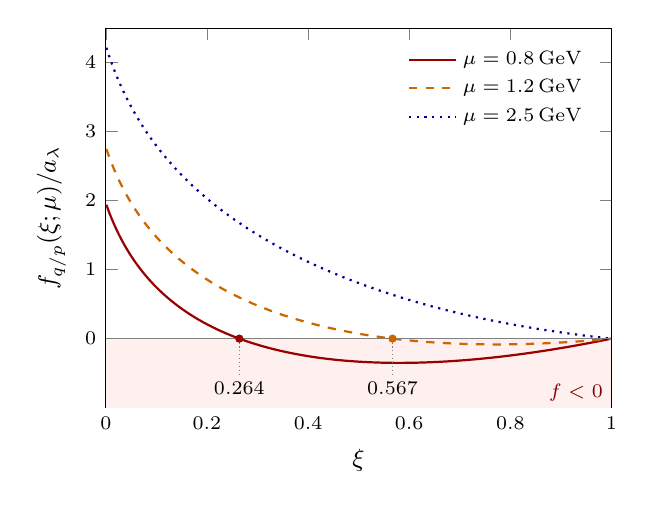
\begin{tikzpicture}
\begin{axis}[width=0.66\textwidth,height=6.4cm,xmin=0,xmax=1,ymin=-1.0,ymax=4.5,
  xlabel={$\xi$},ylabel={$f^{\MSbar}_{q/p}(\xi;\mu)/a_\lambda$},
  xtick={0,0.2,0.4,0.6,0.8,1},ytick={0,1,2,3,4},
  tick label style={font=\scriptsize},label style={font=\small},
  legend style={font=\scriptsize,draw=none,fill=none,at={(0.97,0.97)},anchor=north east},
  legend cell align=left]
\fill[red!6] (axis cs:0,-1.0) rectangle (axis cs:1,0);
\addplot[domain=0.001:0.999,samples=200,thick,red!60!black]{(1-x)*(ln(0.8^2/(2.25*x+0.09*(1-x)-x*(1-x)))-1+(0.3+x)^2/(2.25*x+0.09*(1-x)-x*(1-x)))};
\addlegendentry{$\mu=0.8\,\mathrm{GeV}$}
\addplot[domain=0.001:0.999,samples=200,thick,dashed,orange!80!black]{(1-x)*(ln(1.2^2/(2.25*x+0.09*(1-x)-x*(1-x)))-1+(0.3+x)^2/(2.25*x+0.09*(1-x)-x*(1-x)))};
\addlegendentry{$\mu=1.2\,\mathrm{GeV}$}
\addplot[domain=0.001:0.999,samples=200,thick,dotted,blue!60!black]{(1-x)*(ln(2.5^2/(2.25*x+0.09*(1-x)-x*(1-x)))-1+(0.3+x)^2/(2.25*x+0.09*(1-x)-x*(1-x)))};
\addlegendentry{$\mu=2.5\,\mathrm{GeV}$}
\draw[gray,thin] (axis cs:0,0) -- (axis cs:1,0);
\draw[gray,densely dotted] (axis cs:0.264,0) -- (axis cs:0.264,-0.56);
\draw[gray,densely dotted] (axis cs:0.567,0) -- (axis cs:0.567,-0.56);
\fill[red!60!black] (axis cs:0.264,0) circle[radius=1.5pt];
\fill[orange!80!black] (axis cs:0.567,0) circle[radius=1.5pt];
\node[font=\scriptsize,anchor=north,inner sep=1.5pt] at (axis cs:0.264,-0.56) {$0.264$};
\node[font=\scriptsize,anchor=north,inner sep=1.5pt] at (axis cs:0.567,-0.56) {$0.567$};
\node[font=\scriptsize,text=red!50!black,anchor=south east,inner sep=2pt] at (axis cs:0.995,-1.0) {$f<0$};
\end{axis}
\end{tikzpicture}
\caption{Yukawa 模型中单圈 $\MSbar$ “夸克在核子中”的分布（$m_q=0.3\,\mathrm{GeV}$、$m_p=1.0\,\mathrm{GeV}$、$m_s=1.5\,\mathrm{GeV}$，纵轴以 $a_\lambda=\lambda^2/(16\pi^2)$ 为单位）\cite{CollinsRogersSato2022}：$\mu=0.8\,\mathrm{GeV}$ 时 $\xi>0.264$ 处为负，$\mu=1.2\,\mathrm{GeV}$ 时 $\xi>0.567$ 处为负，$\mu=2.5\,\mathrm{GeV}$ 时处处为正（曲线由 VF-FRO-10 的单圈公式计算）。
“$\MSbar$ 分布在所有标度上非负”因而不成立；足够大标度上的正定性只有部分论证（\cref{prop:front-positivity-large-scale}），一般陈述仍是猜想（\cref{conj:pdf-positivity}）。}
\label{fig:front-yukawa-pdf}
\end{figure}
%%% END fig:front-yukawa-pdf

\begin{example}[Yukawa 模型分布的端点行为与符号变化]\label{ex:front-yukawa}
$\xi\to0$：$\Delta\to m_q^2$，$(m_q+\xi m_p)^2/\Delta\to1$，方括号 $\to\ln(\mu^2/m_q^2)$，当且仅当 $\mu<m_q$ 时为负。$\xi\to1$：$\Delta\to m_s^2$，方括号 $\to\ln(\mu^2/m_s^2)-1+(m_q+m_p)^2/m_s^2$，在 $\mu_*^2=m_s^2\ee^{1-(m_q+m_p)^2/m_s^2}$ 处为零；对上述质量，$\mu_*=1.5\,\ee^{\frac12(1-1.69/2.25)}\,\mathrm{GeV}=1.70\,\mathrm{GeV}$。\cref{fig:front-yukawa-pdf}画出三个标度上的曲线：$\mu=0.8\,\mathrm{GeV}$ 的曲线在 $\xi\approx0.58$ 处取最小值约 $-0.35\,a_\lambda$。
\uses{prop:front-msbar-negative}
\end{example}

\begin{proposition}[足够大标度上的正定性 \tagP]\label{prop:front-positivity-large-scale}
设 (PS1) 一组正的观测量（如 DIS 结构函数，\cref{thm:pdf-dis-xspace}）在领头幂次共线因子化，并定义一个“物理”方案；(PS2) 高扭度可忽略；(PS3) NLO 方案变换是微扰的（\cref{rem:pdf-schemes}）。则 $\MSbar$ PDF 在某个标度以上为正；由于对角道 $\order{\alpha_s}$ 项的 Sudakov 符号（$\MSbar$ 对共线奇异性减多了，而对角道中它们具有 Sudakov 符号），该标度在大 $x$ 处与 $x$ 无关；\cite{Candido:2023ujx}保守地估计为 $Q^2\gtrsim5\,\mathrm{GeV}^2$（来自 $x\sim0.3$、$\alpha_s\lesssim0.2$ 时 $\frac{\alpha_s}{2\pi}C_{gg}(x)<1$）。\cite{CollinsRogersSato2022}定性上同意：“once the $\overline{\rm MS}$ scale is large enough compared with intrinsic transverse momentum scales, the pdfs indeed become positive”。非微扰地位：\cref{asm:intro-wightman}、\cref{asm:intro-composite}、\cref{asm:intro-bridge}（MA0、MA1+MA2）。
\uses{thm:pdf-dis-xspace, rem:pdf-schemes}
\end{proposition}

\paragraph{地位与缺口。}[P]：在 (PS1)--(PS3) 之下的 NLO 论证，高阶与幂次修正不受控制，阈值标度是非微扰的。

\begin{remark}[对本书与拟合的后果]\label{rem:front-positivity-tracks}
(1) $\MSbar$ PDF 的正定性与 Soffer 型不等式在本书中从不作为定理陈述（\cref{prop:coll-soffer}只断言领头阶演化保持后者）；(2) 在低输入标度上把正定性作为拟合约束是一种理论偏置\cite{CollinsRogersSato2022}；(3) 固定阶因子化截面可以为负而不矛盾\cite[附录~A]{CollinsRogersSato2022}；(4) 正的方案（$k_T$ 截断、物理方案）存在——在模型中单圈显式成立（\cref{prop:front-msbar-negative}的证明），其他情形只有一般论证。
\end{remark}

% -----------------------------------------------------------------------------------------------------
\section{算符的 BRST 分类：非定域缺口}\label{sec:front-brst}

\begin{remark}[为什么需要 BRST：K 胶子与非定域缺口]\label{rem:front-k-gluon}
在 Feynman 规范中，DIS 的领头区域含任意多个附着于硬部的纵向极化（“K”）胶子。图形化的非阿贝尔 Ward 恒等式证明\cite{Labastida:1984gy}（\cite[第~11.9~节]{Collins2011}）只在严格共线极限下成立，余项在领头幂次不为零：纯 K 胶子项经由胶子横动量对胶子密度有贡献（显式计算见\cite{Collins:2008sg}），这是构造规范不变胶子 PDF 所需的非阿贝尔效应。Collins 因此改走 BRST 路线\cite[第~11.3.2~节，第~407--410~页]{Collins2011}：对离壳 Green 函数 $T^{\mu\nu}_{\rm off\text{-}shell}(q)=\frac1{4\pi}\int\dd^4z\,\ee^{\ii q\cdot z}\langle0|T\,\text{fields}\,j^\mu(z/2)j^\nu(-z/2)|0\rangle$（其式 (11.11)），领头区域给出 $\sum_iC_i\otimes\langle0|T\,\text{fields}\,O_i|0\rangle$（式 (11.12)），其中 $O_i$ 先验地是光线上“arbitrarily complicated multilocal operators”；Green 函数（式 (11.13)）与流的 BRST 不变性给出 $\delta_{\rm BRST}\sum_iC_i\otimes O_i=0$（式 (11.17)）。对\emph{定域}算符，BRST 不变 $=$ 规范不变 $\oplus$ (A) BRST 变分 $\oplus$ (B) 由运动方程为零的算符（\cite{Joglekar:1975nu}，以及 Collins 所引的\cite{Joglekar:1976eb,Joglekar:1976pe,Nakanishi:1990qm}；作为定域 BRST 上同调的定理见\cite{Henneaux:1993jn,Barnich:2000zw}；Ward 恒等式与背景场规范见\cite{Kluberg-Stern:1974iel,Kluberg-Stern:1974nmx,Kluberg-Stern:1975ebk}，最早的显式规范变异抵消项见\cite{DixonTaylor1974}）——核心陈述是\cref{prop:appJ-local-operators}（[R, $R_{\mathrm{PT}}$]）；A、B 两类在物理矩阵元中为零。缺口的原文（第~410~页）：“Unfortunately, the published proofs that BRST-invariant operators are either gauge invariant or are in one of classes A or B apply as written to local operators. It is natural that the result also applies to the non-local operators we use in factorization. But, as far as I know, no proof has been given. For the purposes of the discussion, I will assume the result is true, and leave the proof (or refutation) to future research.”超出单圈的离壳计算需要 A、B 类算符\cite{Hamberg:1991qt,Collins:1994ee}；规范变异抵消项的全圈结构见\cite{Falcioni:2022fdm}（显式基到四圈）与\cite{Gehrmann:2023ksf}（三圈单态反常维度）（均据摘要）。光锥规范 $A^+=0$ 消去 K 胶子，但 Collins 写道，“given the known problems with $A^+=0$ gauge, it would be nice to have a proof that does not rely on the gauge”。即使承认规范不变性，Wilson 线的路径也要由其余要求确定：共线 PDF 是直的类光线，TMD 则是依赖过程的订书钉形路径。
\end{remark}

\begin{proposition}[双局域 PDF 算符 BRST 分类的矩约化 \tagA]\label{prop:front-brst-bilocal}\hfill\break
令 $O_q(w^-)=\bar\psi(w)\gamma^+W[w,0]\psi(0)$，$w=(0^+,w^-,\mathbf 0_T)$，$O_g(w^-)$ 为相应的胶子算符（\cref{def:pdf-lightray}）。在物理（在壳、BRST 不变）矩阵元中，于重整化微扰论的每一阶，$O^R=Z_{OO}\otimes O_{(0)}$，且
\begin{equation}\label{eq:front-moment-reduction}
\int_0^1\dd z\,z^{N-1}Z_{OO}(z)=Z^{(N)}_{\rm twist\text{-}2}\qquad\text{对一切 }N ,
\end{equation}
BRST 恰当类（A）与运动方程类（B）的混入不出现，$Z_{OO}$ 由其矩唯一确定（紧支；对 $C$ 偶、$C$ 奇组合 $q\pm\bar q$ 与胶子只出现偶数或奇数的 $N$，唯一性由\cref{thm:appK-muntz}给出，至多相差 $z=0$ 处的分布）。因此三角混合（\cite[式~(11.20)]{Collins2011}）
\begin{equation}\label{eq:front-triangular}
\begin{pmatrix}O\\A\\B\end{pmatrix}=\begin{pmatrix}Z_{OO}&Z_{OA}&Z_{OB}\\0&Z_{AA}&Z_{AB}\\0&0&Z_{BB}\end{pmatrix}\begin{pmatrix}O_{(0)}\\A_{(0)}\\B_{(0)}\end{pmatrix}
\end{equation}
限制在物理矩阵元上对双局域 PDF 算符成立。所用输入：$\bar\psi\gamma^+(\ii D^+)^{N-1}\psi$ 与 $F^{+\mu}(\ii D^+)^{N-2}F^+{}_\mu$ 的定域分类（指标全为“$+$”，因而自动对称无迹，恰为扭度 2 算符，\cref{prop:appJ-local-operators}）；前向矩阵元逐阶支撑在 $[-1,1]$（\cref{thm:pdf-support-pt}）；裸非定域算符是裸定域算符的母函数（\cref{prop:appL-bare}；对紧支分布精确，因为其 Fourier 变换是整函数，Taylor 系数即矩）；重整化的矩关系（\cref{prop:appL-renormalized}）。（本命题只涉及算符与部分子态。）
% VF-FRO-15
\uses{def:pdf-lightray, prop:appJ-local-operators, thm:pdf-support-pt, prop:appL-bare, prop:appL-renormalized, thm:appK-muntz}
\end{proposition}

\begin{proofsketch}
(1)~裸双局域算符的矩就是裸定域扭度 2 算符（\cref{prop:appL-bare}）。(2)~由定域分类，$[O_N]=Z_NO_N^{\rm bare}+(\text{A 类})+(\text{B 类})$，且混合是三角的；在物理矩阵元中只剩 $Z_N\equiv Z^{(N)}_{\rm twist\text{-}2}$（\cref{prop:appJ-local-operators}）。(3)~紧支意味着双局域算符的物理矩阵元由其全部矩决定（\cref{thm:pdf-support-pt}）。(4)~在每个 $C$ 宇称扇区（单态为夸克—胶子矩阵）逐阶存在 $[0,1]$ 上的分布 $Z_{OO}$，其 Mellin 矩为 $Z_N$（单圈由 $[(1+z^2)/(1-z)]_+$ 构成）；唯一性：扇区内由\cref{thm:appK-muntz}在 $(0,1]$ 上唯一，在 $[-1,1]$ 上取全部 $N$ 则只需紧支。(5)~重整化的矩关系（\cref{prop:appL-renormalized}）把 (1)--(4) 合成 $O^R=Z_{OO}\otimes O_{(0)}$，即\cref{eq:front-moment-reduction}与限制在物理矩阵元上的\cref{eq:front-triangular}。单圈情形可以逐图核对：由算符定义算出的单圈核的 Mellin 矩等于定域扭度 2 算符的单圈反常维度（第八章）。
\end{proofsketch}

\paragraph{地位与缺口。}[A]。这一约化有先行工作：一般非前向形式是\cite[式~(2.4)、(2.6)、(3.1)、(3.2)]{Braun:2019qtp}（光线算符作为定域算符的母函数，重整化的光线算符由重整化的定域算符同样定义，Joglekar--Lee 分解），思想可追溯到\cite{Balitsky:1987bk}；本书不把它当作新结果。所有输入在本书中都是 [R] 或数学，但我们没有逐行核查附录~L 中\cref{prop:appL-renormalized}的证明不预设非定域算符的分类（循环性问题），这是最弱的一步（代数约化，误差类型不适用）；因此不升级为 [R]。保留：对维数正规化中前向在壳部分子矩阵元，BRST 类与运动方程类不一定为零。它\emph{不}覆盖：因子化证明\emph{内部}的分类一步（规范不变性施加之前、场位于不同光锥位置的多局域算符，\cref{conj:front-brst-multilocal}）；TMD 算符（订书钉路径与快度发散，是另一个问题）；光线算符本身的离壳重整化（物理预言不需要）。

\begin{conjecture}[多局域光线算符的 BRST 分类 \tagC]\label{conj:front-brst-multilocal}
在离壳 Green 函数的领头区域分解（\cite[式~(11.12)]{Collins2011}）中出现的那类、支撑在一条类光线上、鬼数为零的 BRST 不变多局域算符，都等于一个规范不变算符、一个 BRST 变分（A 类）与一个由运动方程为零的算符（B 类）之和。
\uses{def:prelim-brst, prop:appJ-local-operators}
\end{conjecture}

\paragraph{地位与缺口。}[C]：Collins 假定了它（\cref{rem:front-k-gluon}中的原文）；据我们截至 2026 年 10 月的文献检索（INSPIRE 与网络检索），尚未见非定域（多局域）BRST 分类的证明。在因子化证明中它以被明确假定的一步\cref{asm:appN-brst-nonlocal}（[C]）出现。自然的工具是用辅助场局域化（把 Wilson 线当作一个场），如同类空 Wilson 线算符的可重整性论证\cite{Ji:2017oey,Ishikawa:2017faj,Green:2017xeu}（\cref{prop:lattice-renormalizability}，\cref{asm:lamet-aux-renorm}）。“Collins（2011）证明了非定域算符的 BRST 分类”是过度表述；附录~J 的\cref{rem:appJ-nonlocal}指向这里与\cref{prop:front-brst-bilocal}。

% -----------------------------------------------------------------------------------------------------
\section{小 $x$：Wilson 线（高能）因子化的地位}\label{sec:front-smallx}

小 $x$ 的“因子化”是与共线因子化不同的展开：Regge 极限 $s\gg|t|$（DIS 中 $Q^2$ 固定而 $x\to0$），由 Wilson 线的快度因子化（激波图像）组织——入射体的冲击因子 $\otimes$ 在快度上演化（BK/JIMWLK）的靶 Wilson 线关联函数。它的结果是在程函（Regge）展开之内、固定对数精度上的全阶陈述，而不是有幂次计数控制的领头幂次定理；下面的分级都是相对于这一框架的。领头阶 BK 方程是\cref{thm:smallx-bk}，此处不重述。

\begin{proposition}[NLO BK/JIMWLK 与三圈 BK 核 \tagA]\label{prop:front-nlo-bk}
在程函（Regge）展开的次领头对数精度上：(a) 色偶极子的 NLO 演化含二次与三次非线性；NLO 核是跑动耦合部分（$\propto\beta_0$）、共形部分（$1\to3$ 偶极子跃迁）与一个非共形双对数项之和；其前向线性化与 NLO BFKL 核一致\cite{Balitsky:2007feb}——该文第~VI~节与结论（第~VIII~节）报告的 $\alpha_s^2\zeta(3)\times$（偶极子）的差异，后被同一作者追溯到一个被假定为零的积分的错误求值，修正后消失\cite[第~6~节，“In QCD”]{Balitsky:2009xg}；夸克部分与跑动耦合见\cite{Balitsky:2006wa,Kovchegov:2006vj}；(b) NLO JIMWLK\cite{Balitsky:2013fea,Kovner:2013ona}，其共形对称性\cite{Kovner:2014xia}与“unabridged”形式\cite{Kovner:2014lca}（据摘要）；(c) 平面 $\mathcal N=4$ 超对称 Yang--Mills 中的三圈 BK 核，借助与非全局对数的等价、一种 Lorentz 协变的红外／共线减除方法得到，并与 Pomeron 轨迹和扭度 2 谱核对（\cite{Caron-Huot:2016tzz}，据摘要）。（本命题是关于 Wilson 线算符的演化方程。）
\uses{thm:smallx-bk, thm:smallx-bfkl}
\end{proposition}

\begin{proofsketch}
在激波背景中计算 Wilson 线偶极子的单圈修正（胶子与夸克圈、两个胶子的发射），分离跑动耦合与共形部分，再取线性化前向极限与 NLO BFKL 比较。完整论证见\cite{Balitsky:2007feb,Balitsky:2009xg}。
\end{proofsketch}

\paragraph{地位与缺口。}[A]，在程函框架之内。本书不把它当作与 NLO BFKL 的分歧：\cite{Balitsky:2007feb}中的 $\zeta(3)$ 项已被作者撤回\cite[第~6~节]{Balitsky:2009xg}，也不应归因于纵向截断。

\begin{proposition}[NLO BK 的不稳定性与共线重求和 \tagP]\label{prop:front-bk-collinear}
对现实的初始条件，NLO BK 方程的解不稳定\cite{Lappi:2015fma}；运动学约束与共线重求和可以消除这一不稳定性\cite{Beuf:2014uia,Iancu:2015vea}（均据摘要）。
\uses{prop:front-nlo-bk}
\end{proposition}

\paragraph{地位与缺口。}[P]：各种重求和处方在受控对数之外互不相同；与方案无关的共线改进仍是开放问题（\cref{rem:front-open}）。

\begin{proposition}[{\small 高能极限中的 Wilson 线方法、胶子 Regge 化与 Regge 极限的红外奇异部分} \tagA]\label{prop:front-regge}\hfill\break
(a) 带快度依赖的 Wilson 线集合的程函近似（Balitsky--JIMWLK）再现胶子 Regge 化与 BFKL；从四圈起，BFKL 动力学与红外发散的偶极子公式不相容；在严格平面极限下，理论可以用有限个、依赖过程的 Wilson 线表述而不提及 Regge 化胶子，并在 $\mathcal N=4$ 中精确核对（\cite{Caron-Huot:2013fea}，据摘要，第~4~节已核对）。(b) 高能极限下 $2\to2$ 振幅的红外奇异部分在次领头对数精度上有全阶闭式（双 Reggeon 贡献），预言软反常维度在任意圈数的 Regge 极限（\cite{Caron-Huot:2017zfo}，据摘要）。（本命题只涉及部分子振幅。）
\uses{thm:smallx-bfkl, thm:sudakov-ir-poles}
\end{proposition}

\begin{proofsketch}
把振幅写成快度分级的 Wilson 线关联函数，用 Balitsky--JIMWLK 演化逐阶生成高能对数，并与红外因子化（\cref{thm:sudakov-ir-poles}）的结构比较。完整论证见所引文献。
\end{proofsketch}

\paragraph{地位与缺口。}[A]：程函（Regge）展开之内、固定对数精度上的全阶论证；(a) 只在平面 $\mathcal N=4$ 中精确核对，(b) 在次领头对数精度上对全阶成立；部分来源只读到摘要层次。这不是 QCD 的领头幂次定理：“BK/JIMWLK 是 QCD 的领头幂次定理”是过度表述。

\begin{proposition}[简单 Regge 极点因子化在 NNLL 失效 \tagV]\label{prop:front-regge-pole}
利用红外因子化，$2\to2$ 振幅最简单的 Regge 极点因子化在 $\ln(s/|t|)$ 的次次领头对数（NNLL）精度失效：出现两圈的非对数双极点与三圈的不因子化单对数奇异项；直到次领头对数，硬函数在 $d=4$ 中对全阶为零（\cite{DelDuca:2013ara,DelDuca:2014cya}，据该文摘要）。
\uses{def:smallx-regge, thm:sudakov-ir-poles}
\end{proposition}

\paragraph{地位与缺口。}对超出次领头对数的 Regge 极点因子化为 [V]，证据：基于红外因子化（\cref{thm:sudakov-ir-poles}，[A]）的显式计算；修正后的多 Reggeon 图像是 [A]（\cref{prop:front-regge}(b)）。

\begin{proposition}[小 $x$ 的 TMD 与 Sudakov 对数 \tagA]\label{prop:front-smallx-tmd}
在色玻璃凝聚框架的领头阶与领头对数精度上（均据摘要）：(a) 稀—密碰撞中双喷注的有效 $k_t$ 因子化；Weizsäcker--Williams 与偶极子胶子分布是普适的小 $x$ TMD，在小 $x$ 带依赖过程的规范链\cite{Dominguez:2011wm}；(b) 在饱和形式中把 Sudakov 双对数与小 $x$ 重求和结合\cite{Mueller:2012uf}。(c)（部分结果，\tagP）胶子 TMD 从小 $x$ 到中等 $x$ 的快度演化\cite{Balitsky:2015qba}；小 $x$ 的规范不变 TMD 因子化、只按快度的因子化与 Sudakov--BFKL 插值\cite{Balitsky:2020jzt,Balitsky:2021fer,Balitsky:2023hmh,Balitsky:2026lop}。（高能展开框架内的陈述；靶的非微扰信息作为初始条件输入。）
\uses{thm:smallx-bk}
\end{proposition}

\begin{proofsketch}
在激波背景中计算双喷注截面并在相关极限下与 TMD 形式匹配，识别出两种胶子分布及其规范链；Sudakov 对数由软胶子在饱和背景中的再求和得到。完整论证见所引文献。
\end{proofsketch}

\paragraph{地位与缺口。}(a)(b) 为 [A]（领头阶／领头对数），(c) 为 [P]。

\begin{proposition}[小 $x$ 螺旋度演化：截距与 BER 的分歧 \tagA]\label{prop:front-smallx-helicity}
在双对数近似与大 $N_c$（或大 $N_c\&N_f$）下（据该文摘要），小 $x$ 的螺旋度演化（双对数 $\alpha_s\ln^2(1/x)$）由极化偶极子振幅即次程函 Wilson 线算符给出\cite{Kovchegov:2015pbl,Kovchegov:2016weo}（前者连同勘误），其修正形式见\cite{Cougoulic:2022gbk}；大 $N_c$ 下的精确解给出 $\Delta\Sigma\sim\Delta G\sim g_1\sim(1/x)^{\alpha_h}$，
\begin{equation}\label{eq:front-helicity}
\alpha_h\simeq3.66074\sqrt{\frac{\alpha_sN_c}{2\pi}}\quad\text{\cite{Borden:2023ugd}},\qquad
\alpha_h^{\rm BER}\simeq3.66394\sqrt{\frac{\alpha_sN_c}{2\pi}}\quad\text{（红外演化方程\cite{Bartels:1996wc}）}.
\end{equation}
所求和的 $\Delta\gamma_{GG}(\omega)$ 与固定阶反常维度一致到三圈，从四圈起与 Bartels--Ermolaev--Ryskin（BER）\cite{Bartels:1995iu,Bartels:1996wc}的结果不同；大 $N_c\&N_f$ 见\cite{Adamiak:2023okq}、\cite{Borden:2024bxa}（夸克$\leftrightarrow$胶子跃迁算符）与\cite{Borden:2025ehe}（解析解；与 BER 及 Blümlein--Vogt\cite{Blumlein:1996hb}的细微分歧仍在）。（高能展开框架内的陈述。）
% VF-FRO-17 (formulas typeset with \cite, not \texttt)
\uses{thm:smallx-bk, def:pdf-polarized}
\end{proposition}

\begin{proofsketch}
写出极化偶极子振幅的演化方程（大 $N_c$ 下闭合），在双对数近似下精确求解，读出 Mellin 空间的 $\Delta\gamma_{GG}$ 与其最右奇点。按\cite{Borden:2023ugd}的记法，$\bar a=\alpha_sN_c/(2\pi)$，
\begin{equation}\label{eq:front-dgamma}
\Delta\gamma_{GG}=\frac\omega2\Bigl[1-\sqrt{1-\tfrac{16\bar a}{\omega^2}\sqrt{1-\tfrac{4\bar a}{\omega^2}}}\,\Bigr],\qquad
\Delta\gamma_{GG}^{\rm BER}=\frac\omega2\Bigl[1-\sqrt{1-\tfrac{16\bar a}{\omega^2}\tfrac{1-3\bar a/\omega^2}{1-\bar a/\omega^2}}\,\Bigr]
\end{equation}
（后者为该文转写的 BER 纯胶子大 $N_c$ 形式），展开为 $\Delta\gamma_{GG}=\frac{4\bar a}\omega+\frac{8\bar a^2}{\omega^3}+\frac{56\bar a^3}{\omega^5}+\frac{496\bar a^4}{\omega^7}+\cdots$，BER 的第四项系数为 $504$。截距是外层根号的零点：令 $u=\omega^2/\bar a$，分别得 $u^3-256u+1024=0$ 与 $u^2-17u+48=0$，最大根给出 $\sqrt u=3.66074$ 与 $\sqrt{(17+\sqrt{97})/2}=3.66394$（BER 原文只给出 $3.66$）。完整论证见\cite{Borden:2023ugd,Borden:2025ehe}。
% check: writing/work/W27/s_helicity.py (coefficients 4,8,56,496,4824 vs 4,8,56,504,4920; intercepts)
\end{proofsketch}

\paragraph{地位与缺口。}[A]（双对数近似，大 $N_c$ 或大 $N_c\&N_f$）；与 BER 的分歧是开放问题，本书不作裁决（2026 年的现状见\cite{Borden:2025ehe}）。相关工作（据摘要）：小 $x$ 的胶子轨道角动量\cite{Hatta:2016aoc}与胶子 GPD $E_g$ 的小 $x$ 演化\cite{Hatta:2022bxn}，在相应近似下属全阶论证或部分结果。

% -----------------------------------------------------------------------------------------------------
\section{双部分子散射}\label{sec:front-dps}

一次 $pp$ 碰撞中的两个硬散射（如双 Drell--Yan）对积分截面形式上是幂次压低的，但对横动量微分截面（$q_{T,i}\ll Q_i$）是领头的，在小 $x$ 多末态时还会增强。框架（据各文摘要）：色关联的双部分子分布（DPD）、幂次计数、全阶证明的要素以及与 GPD 和格点的联系\cite{DiehlOstermeierSchafer2012}（连同勘误）；色关联、干涉、演化、$1\to2$ 劈裂奇异性（小间距 $y$ 处 $\propto1/y^2$）与重复计数问题\cite{Manohar:2012jr,Manohar:2012pe}。双 Drell--Yan 中积分截面与 $q_T$ 微分截面的全阶 Glauber 相消\cite{Diehl:2015bca}，以及借非阿贝尔 Ward 恒等式使软胶子退耦为 Wilson 线真空期望值\cite{Diehl:2018wfy}，属于核心陈述\cref{thm:break-double-dy}（[A]）。

\begin{proposition}[无重复计数的双部分子散射 \tagA]\label{prop:front-dps-scheme}
\begin{equation}\label{eq:front-dgs}
\sigma=\sigma_{\rm SPS}+\sigma_{\rm DPS}-\sigma_{\rm sub},\qquad
\frac{\dd\sigma_{\rm DPS}}{\dd x_1\dd x_2\dd\bar x_1\dd\bar x_2}=\sum\hat\sigma_{a_1b_1}\hat\sigma_{a_2b_2}\!\int\!\dd^2y\,\Phi^2(y\nu)F_{b_1b_2}(\bar x_i,y)F_{a_1a_2}(x_i,y),
\end{equation}
其中截断函数满足 $u\gg1$ 时 $\Phi(u)\to1$、小 $u$ 时 $\Phi(u)=\order{u^\delta}$（如 $\Theta(u-b_0)$ 或 $1-\ee^{-u^2/4}$），$\nu\sim Q$；$\sigma_{\rm sub}$ 是把两个 DPD 都换成其固定阶微扰劈裂形式的 DPS 公式（对 1v1 即 $\sigma_{1v1,{\rm pt}}$）。小 $y$ 处 $\Phi$ 依赖在 $\sigma_{\rm DPS}$ 与 $\sigma_{\rm sub}$ 之间相消（剩下 SPS），大 $y$ 处 $\sigma_{\rm SPS}\simeq\sigma_{\rm sub}$（剩下 DPS）。由此 DPD 被定义为可在高阶使用的算符矩阵元\cite[第~4.1~节]{Diehl:2017kgu}。非微扰地位：\cref{asm:intro-composite}、\cref{asm:intro-bridge}（MA0、MA1+MA2）。
% VF-FRO-13
% errtype: E-S
\uses{def:break-dpdf, thm:break-double-dy}
\end{proposition}

\begin{proofsketch}
把 DPS 区域与 SPS 中 $1\to2$ 劈裂区域的重叠写成以 $\Phi$ 截断的 $y$ 积分，在小 $y$ 处用 DPD 的微扰劈裂形式构造减除项 $\sigma_{\rm sub}$，逐阶检验两端极限中 $\Phi$ 依赖的相消。完整论证见\cite[第~4~节]{Diehl:2017kgu}。
\end{proofsketch}

\paragraph{地位与缺口。}[A]：方案的自洽性在固定阶论证；DPD 演化之后，相消只在更高阶意义下成立。带色末态或喷注的完整 DPS 因子化仍是猜想（\cref{conj:break-dps-coloured}）。

\begin{proposition}[多部分子软因子快度发散的重整化定理 \tagA]\label{prop:front-rapidity-renorm}
多部分子软因子的快度发散来自与无穷远横平面的交换，经一个共形映射在结构上等价于紫外发散；由此得到快度发散的重整化定理（借共形变换证明）、多部分子 TMD 的定义，以及软反常维度与快度反常维度之间的精确关系（并导出三圈快度反常维度）（\cite{Vladimirov:2017ksc}，据该文摘要）。（本命题只涉及软因子即 Wilson 线真空期望值。）
\uses{def:tmd-soft, def:break-dpdf}
\end{proposition}

\begin{proofsketch}
用共形变换把类光 Wilson 线软因子中远横平面处的快度发散映到紫外发散，再搬用 Wilson 线算符的紫外重整化定理。完整论证见\cite{Vladimirov:2017ksc}。
\end{proofsketch}

\paragraph{地位与缺口。}[A]（只读到摘要层次）。第二十二、二十三章关于快度发散线性性的讨论指向这里；Vladimirov 称 SIDIS 软因子的快度因子化是“the open question”（据\cite{Liu:2023pjb}引用的\cite{Vladimirov:2017ksc}期刊版第~32~页）。

\begin{proposition}[色关联 DPD 的演化与匹配 \tagP]\label{prop:front-dpd-evolution}
到次领头阶（两圈核），均据摘要：TMD DPS 的因子化、演化与匹配\cite{Buffing:2017mqm}（连同 2021 年的勘误／增补）；色非单态 DPD 的 NLO 演化核\cite{Diehl:2022rxb}；两圈 $1\to2$ 劈裂\cite{Diehl:2019rdh}；劈裂中的夸克质量效应\cite{Diehl:2022dia}；坐标空间中的动量与数目求和规则\cite{Diehl:2020xyg}；综述\cite{Diehl:2017wew}。（本命题只涉及演化核与部分子层次的匹配系数。）
\uses{def:break-dpdf, prop:front-rapidity-renorm}
\end{proposition}

\paragraph{地位与缺口。}[P]（算到 NLO）；色关联 DPD 的唯象仍是开放问题。

% -----------------------------------------------------------------------------------------------------
\section{喷注、喷注子结构与非全局观测量}\label{sec:front-jets}

带非全局对数的 $e^+e^-$ 喷注过程的因子化定理\cite{Becher:2015hka,Becher:2016mmh}——硬函数 $\mathcal H_m$ 乘多 Wilson 线软函数 $\mathcal S_m$，重整化群方程是多重数空间中的矩阵，领头对数与大 $N_c$ 下给出 BMS 方程，窄锥时出现 coft 模式——是核心陈述\cref{thm:jets-ngl-factorization}（[A]）；轻喷注质量与半球软函数\cite{Becher:2016omr}亦然。本节记录超出它的结果；在强子对撞中 Glauber 相位产生超领头对数（\cref{sec:front-sll}）。

\begin{proposition}[非全局对数：超出领头对数与测量驱动的因子化 \tagA]\label{prop:front-ngl}
(a) 色密度矩阵在一切对数阶重求和非全局对数，其反常维度已知到 LO 与 NLO；经共形变换它等价于激波（Regge）演化，重新导出 NLO BFKL／Balitsky--JIMWLK，并在一切对数阶证明发散的指数化（\cite{Caron-Huot:2015bja}，据摘要）。(b) 在大 $N_c$ 与次领头对数精度上，非全局对数的 NLL 重求和：平面大 $N_c$ QCD 中的积分—微分方程，以维数正规化形式与显式有限的四维形式给出，并在 $\order{\alpha_s^2}$ 与完整 QCD 核对\cite{Banfi:2021owj}；喷注演算\cite{Banfi:2021xzn}；两圈反常维度\cite{Becher:2021urs}；以大 $N_c$ 部分子簇射实现的 LHC 上的 NLL 重求和\cite{Becher:2023vrh}；2026 年关于非全局与聚类对数的两圈反常维度\cite{Becher:2026zon}以及 Higgs 产生中 NLL 非全局对数\cite{Becher:2026iim}的预印本（均据摘要）。(c) 通过足够多的测量（“修饰胶子”），非全局对数可以因子化并重求和到一个未分辨的标度（\cite{Larkoski:2015zka}，据摘要）。（本命题只涉及部分子截面。）
% errtype: E-S
\uses{thm:jets-ngl-factorization, thm:jets-bms}
\end{proposition}

\begin{proofsketch}
(a) 把软辐射写成作用于 Wilson 线色密度矩阵的演化，经共形映射与激波演化对应；(b) 在大 $N_c$ 下推导并数值求解 NLL 的演化方程，与固定阶核对；(c) 增加测量把非全局结构化为全局的。完整论证见所引文献。
\end{proofsketch}

\paragraph{地位与缺口。}[A]（(b) 限于大 $N_c$ 与 NLL；只读到摘要层次）。第十六章的\cref{prop:jets-ngl-beyond}（[P]）涉及有限 $N_c$ 与固定阶结果，与这里限于大 $N_c$ 的 [A] 并不矛盾。

\begin{proposition}[喷注子结构、修饰喷注与半单举喷注函数 \tagA]\label{prop:front-jet-substructure}
(a) 在 soft-drop 幂次计数 $z_{\rm cut}\ll1$ 中，一大类 soft-drop 修饰的观测量（含喷注质量）因子化；修饰掉软宽角辐射后，一切奇异贡献都是共线的，因此归一化分布在所有阶都没有非全局对数，并且除夸克／胶子份额外与过程无关；NNLL 重求和\cite{Frye:2016aiz}。(b) 修饰喷注中的强子化：在中间的喷注质量区，领头幂次修正是三个普适的非微扰参数乘以微扰系数；更小的质量处是一个未归一化的形状函数\cite{Hoang:2019ceu}。(c) 半单举喷注函数 $J_i(z,\omega_J,\mu)$ 精确地服从类时 DGLAP 演化（\cref{prop:pdf-timelike-dglap}；$\ln R$ 的重求和），单举喷注产生与单举强子产生共享硬函数，只需 $D_i^h\to J_i$\cite{Kang:2016mcy}。（均据摘要。本命题只涉及部分子截面；(b) 的非微扰参数作为输入。）
% errtype: E-S
\uses{def:jets-algorithms, prop:pdf-timelike-dglap}
\end{proposition}

\begin{proofsketch}
在 SCET 中按 soft-drop 的幂次计数分离硬、全局软、共线—软与共线模式并逐一因子化；(c) 由喷注函数的单圈计算与重整化群相容性得到。完整论证见所引文献。
\end{proofsketch}

\paragraph{地位与缺口。}[A]（(c) 为 NLO 加重整化群相容性；只读到摘要层次）。

\begin{proposition}[能量关联子的共线因子化与共形场论中的光线 OPE \tagA]\label{prop:front-lightray-ope}
(a) 能量—能量关联子在一般量子场论的共线极限下领头幂次因子化，反常维度由类时劈裂函数的矩给出（\cref{prop:pdf-timelike-dglap}）；QCD 中到 NNLL（\cite{Dixon:2019uzg}，据摘要）。(b) 在共形场论中（非微扰），同一类光平面上的零积分（光线）算符有收敛的 OPE（“光线 OPE”；事件形状的天球块），在非微扰共形场论中用 Lorentz 反演公式导出（\cite{Kologlu:2019mfz}，据摘要）——这是事件形状共线因子化的非微扰类比，而不是 QCD 陈述。（(a) 是微扰陈述；(b) 是共形场论中的非微扰陈述。）
% errtype: E-S
\uses{def:jets-algorithms, prop:pdf-timelike-dglap}
\end{proposition}

\begin{proofsketch}
(a) 用光线算符的 OPE 把能量关联子的共线极限写成扭度 2 光线算符之和，其演化由类时劈裂函数的矩控制；(b) 在共形场论中用 Lorentz 反演公式构造光线算符乘积的收敛展开。完整论证见所引文献。
\end{proofsketch}

\paragraph{地位与缺口。}[A]；(b) 是共形场论中的非微扰结论，也是本章唯一的非微扰正面结论，它不涉及 QCD。

% -----------------------------------------------------------------------------------------------------
\section{重夸克偶素产生：NRQCD 因子化的进展}\label{sec:front-quarkonium}

NRQCD 因子化\cite{BodwinBraatenLepage1995} $\dd\sigma(H)=\sum_n\dd\hat\sigma_n(\Lambda)\langle\mathcal O^H_n(\Lambda)\rangle$ 对衰变是全阶论证（\cref{thm:heavy-nrqcd-decay}，[A]），对产生是猜想（\cref{conj:heavy-nrqcd-production}，[C]）。问题有二：(i) 短程系数的红外发散在所有阶是否与长程矩阵元的相匹配；(ii) 长程矩阵元的普适性。

\begin{proposition}[NNLO 的红外极点与规范完备的八重态算符 \tagP]\label{prop:front-nrqcd-ir}
在 NNLO（两圈）阶（均据摘要）：(a) 大 $p_T$ 胶子碎裂中，NNLO 的红外极点不被通常的色八重态产生算符匹配；规范不变性与因子化要求带 Wilson 线（非阿贝尔相位）的算符，用这些“规范完备”的矩阵元，因子化在 NNLO 恢复，先到 $\order{v^2}$，随后对八重态到单态的跃迁到 $v$ 的所有阶\cite{NayakQiuSterman2005a,NayakQiuSterman2005b,NayakQiuSterman2006}；保留：超出 NNLO，“in the absence of special cancellations”，可能需要 NRQCD 速度展开之外的非定域算符。(b) 对色八重态 S 波对碎裂为任意轨道角动量色单态对的长程矩阵元的协变两圈计算发现，红外发散与 Wilson 线方向无关，正如普适性所要求；结果在某些方面与 NQS 不同（来源已查明），两者都与 NRQCD 因子化相容，而“the general principle that underlies this confirmation \dots\ has yet to be revealed”\cite{Bodwin:2019bpf}。（本命题只涉及部分子层次的匹配。）
\uses{def:heavy-nrqcd}
\end{proposition}

\paragraph{地位与缺口。}[P]（两圈）。“NQS 的规范完备 Wilson 线在 NNLO 不改变结果”是过度表述——它们在 NNLO 是必需的。

\begin{remark}[唯象张力与替代方案]\label{rem:front-quarkonium-alternatives}
在 $1/p_T$ 中领头与次领头幂次的共线（碎裂）因子化（单部分子碎裂与重夸克对碎裂；\cite{Kang:2011mg,Kang:2014tta,Kang:2014pya,Fleming:2012wy,Ma:2013yla,Ma:2014eja,Bodwin:2014gia}）是核心陈述\cref{prop:heavy-quarkonium-fragmentation}（[A]）；它依赖于高 $p_T$ 单举共线因子化，而 Collins 在谈到详细证明的普遍缺乏时，把 NQS 2005 年的论证列为“notable exception”\cite[第~14.7~节，第~570--571~页]{Collins2011}。LHCb 的 $\eta_c$ 数据与重夸克自旋对称：一方认为它“challenges NRQCD factorization”\cite{Butenschoen:2014dra}，另一方得到相容的拟合\cite{Han:2014jya,Zhang:2014ybe}——两方并列，不作裁决；极化之谜仍然存在（此处不评述）。软胶子因子化\cite{Ma:2017xno}（据摘要）不先按相对速度展开就处理软强子化效应，并声称速度收敛更好——这是带部分检验的提议，作为定理属于猜想。
\end{remark}

% -----------------------------------------------------------------------------------------------------
\section{QED 修正、光子与轻子 PDF、电弱因子化}\label{sec:front-qed}

第十一章的\cref{prop:coll-luxqed}（[A]）陈述了质子的光子分布可由结构函数模型无关地确定；这里给出精确公式、它的点状极限检验，以及 QED 与电弱因子化的其他前沿结果。

\begin{theorem}[由结构函数确定质子的光子 PDF（LUXqed） \tagA]\label{thm:front-luxqed}
在 $\MSbar$ 方案中
\begin{equation}\label{eq:front-luxqed}
\begin{split}
xf_{\gamma/p}(x,\mu^2)=\frac{1}{2\pi\alpha(\mu^2)}\int_x^1\frac{\dd z}{z}\Bigl\{&\int_{\frac{x^2m_p^2}{1-z}}^{\frac{\mu^2}{1-z}}\frac{\dd Q^2}{Q^2}\,\alpha^2(Q^2)\Bigl[\Bigl(zp_{\gamma q}(z)+\frac{2x^2m_p^2}{Q^2}\Bigr)F_2\Bigl(\frac xz,Q^2\Bigr)\\
&\qquad\qquad-z^2F_L\Bigl(\frac xz,Q^2\Bigr)\Bigr]\\
&-\alpha^2(\mu^2)\,z^2F_2\Bigl(\frac xz,\mu^2\Bigr)\Bigr\},\qquad zp_{\gamma q}(z)=1+(1-z)^2,
\end{split}
\end{equation}
包含 $\alpha L(\alpha_sL)^n$、$\alpha(\alpha_sL)^n$ 与 $\alpha^2L^2(\alpha_sL)^n$ 量级的全部项（$L=\ln\mu^2/m_p^2$）；$F_{2,L}$ 含弹性部分 $F_2^{\rm el}=\frac{G_E^2+\tau G_M^2}{1+\tau}\delta(1-x)$、$F_L^{\rm el}=\frac{G_E^2}{\tau}\delta(1-x)$，$\tau=Q^2/4m_p^2$\cite[式~(6)]{Manohar:2016nzj}。非微扰地位：\cref{asm:intro-wightman}、\cref{asm:intro-composite}、\cref{asm:intro-bridge}（MA0、MA1+MA2）。
% VF-FRO-11
% errtype: E-S
\uses{def:pdf-gluon, thm:disall-factorization}
\end{theorem}

\begin{proofsketch}
考虑一个虚构的超出标准模型的过程 $l+p\to L+X$，经由跃迁磁矩 $(e/\Lambda)\bar L\sigma^{\mu\nu}F_{\mu\nu}l$。其截面 (i) 可以用 $F_2$、$F_L$ 精确表示（轻子流不被重整化），(ii) 也可以用 $\MSbar$ PDF 的共线因子化（\cref{thm:disall-factorization}）表示，其中光子 PDF 定义为\cref{def:pdf-gluon}的 QED 类比；在所述精度上令二者相等即定出 $f_\gamma$。后续工作\cite{Manohar:2017eqh}（据摘要）由算符定义直接推出该结果，给出对 QED 与 QCD 所有阶（含非微扰修正）用 $F_2$、$F_L$ 表示的精确表达式、高一阶的公式、极化与 TMD 光子分布，以及 $\order{\alpha\alpha_s}$、$\order{\alpha^2}$ 的 $P_{\gamma i}$。完整论证见\cite{Manohar:2016nzj,Manohar:2017eqh}。
\end{proofsketch}

\paragraph{地位与缺口。}[A]：依赖辅助过程的共线因子化（\cref{thm:disall-factorization}，[A]）；由算符定义的推导使它与过程无关。第十一章的光子结构讨论使用同一公式。

\begin{example}[点状靶极限]\label{ex:front-luxqed-pointlike}
对质量为 $m$ 的点状 Dirac 费米子靶（只有弹性部分，$G_E=G_M=1$）：$F_2(x',Q^2)=\delta(1-x')$，$F_L=\frac{4m^2}{Q^2}\delta(1-x')$。由 $\delta(1-x/z)=x\,\delta(z-x)$（弹性 $\delta$ 函数按惯例完整计入），$z$ 积分令 $z=x$，固定 $\alpha$ 时
\begin{equation*}
xf_\gamma=\frac{\alpha}{2\pi}\Bigl\{[1+(1-x)^2]\ln\frac{\mu^2}{x^2m^2}-2x^2m^2\Bigl(\frac{1-x}{x^2m^2}-\frac{1-x}{\mu^2}\Bigr)-x^2\Bigr\},
\end{equation*}
其中第二项来自 $\int\frac{\dd Q^2}{Q^2}\bigl(\frac{2x^2m^2}{Q^2}-x^2\frac{4m^2}{Q^2}\bigr)$，第三项是 $\MSbar$ 换算项。用 $-2(1-x)-x^2=-[1+(1-x)^2]$，
\begin{equation}\label{eq:front-luxqed-point}
xf_\gamma=\frac{\alpha}{2\pi}\bigl[1+(1-x)^2\bigr]\Bigl[\ln\frac{\mu^2}{m^2}-2\ln x-1\Bigr]+\frac{\alpha m^2x^2(1-x)}{\pi\mu^2},
\end{equation}
即\cite[式~(4.189)]{Frixione:2019lga}的 $\order{\alpha}$ $\MSbar$ 轻子中光子分布，外加一个幂次修正。去掉 $F_L$ 项会使常数项移动 $\frac{\alpha}{2\pi}4(1-x)$，去掉 $\MSbar$ 换算项会移动 $\frac{\alpha}{2\pi}x^2$：两者都是检验所必需的。
% check: writing/work/W27/s_series.py (C1)-(C5); frontier check OTHERS s3
\uses{thm:front-luxqed}
\end{example}

\begin{proposition}[轻子与电子的 PDF、QED 与混合演化核 \tagA]\label{prop:front-lepton-pdf}
均据摘要：(a) 由同样的结构函数输入在 NLO 得到质子的轻子 PDF\cite{Buonocore:2020nai}；(b) QED 中电子的电子、正电子与光子 PDF 到 NLL，大 $z$ 全阶重求和并与 $\order{\alpha^3}$ 匹配（初始条件\cite{Frixione:2019lga}；\cite{Bertone:2019hks}连同勘误）；(c) Altarelli--Parisi 核的 QED 修正与 QCD$\times$QED 混合修正：$\order{\alpha\alpha_s}$\cite{deFlorian:2015ujt}与借“阿贝尔化”得到的 $\order{\alpha^2}$\cite{deFlorian:2016gvk}，均为所述阶的显式核。非微扰地位：\cref{asm:intro-bridge}（MA1+MA2；只对 (a)，(b)(c) 只涉及部分子层次的演化）。
% errtype: E-S
\uses{thm:front-luxqed, thm:pdf-dglap}
\end{proposition}

\begin{proofsketch}
(a) 与\cref{thm:front-luxqed}同法，以带电轻子替代光子；(b) 求解 QED 的 DGLAP 方程并在大 $z$ 处重求和，初始条件由固定阶计算给出；(c) 由 QCD 核经色因子替换（阿贝尔化）得到 QED 与混合核。完整论证见所引文献。
\end{proofsketch}

\paragraph{地位与缺口。}[A]（只读到摘要层次）；(c) 是有限阶结果。

\begin{proposition}[电弱 PDF 与 $Q\gg M_W$ 的电弱对数 \tagA]\label{prop:front-ew-pdf}
均据摘要：在 $Q\gg M_W$ 时，电弱 PDF 及其演化重求和电弱对数\cite{Bauer:2017isx}（极化效应\cite{Bauer:2018arx}；由结构函数得到 $W$、$Z$ 的 PDF\cite{Fornal:2018znf}）；在 NLL 框架中，因子化定理中的对象不必是 $SU(2)\times U(1)$ 单态，DGLAP 型演化只对足够单举的测量（如不变质量）捕获全部电弱对数，而识别末态轻子需要碎裂函数与软交换\cite{Manohar:2018kfx}。非微扰地位：\cref{asm:intro-bridge}（MA1+MA2）。
% errtype: E-S
\uses{thm:pdf-dglap}
\end{proposition}

\begin{proofsketch}
在破缺的电弱理论中把 $Q\gg M_W$ 的截面写成 SCET 因子化形式，规范玻色子与费米子都作为部分子，演化核由未破缺的 $SU(2)\times U(1)$ 给出、在 $M_W$ 处匹配。完整论证见所引文献。
\end{proofsketch}

\paragraph{地位与缺口。}[A]（只读到摘要层次）。

\begin{proposition}[电弱 Bloch--Nordsieck 抵消的失效与测量弱荷的观测量 \tagV]\label{prop:front-ew-violation}
(a) 对撞机初态带确定的非阿贝尔（弱同位旋）荷，因此电弱 Sudakov 双对数在 TeV 标度的单举截面中不相消：对非单态初态，Bloch--Nordsieck 抵消失效（\cite{Ciafaloni:2000df}，据该文摘要）。(b) 对强子对撞中测量末态弱荷的观测量，不因子化的电弱修正在领头幂次破坏部分子模型图像，从 $\order{\alpha_s^2\alpha_W^2\log^4(Q^2/M_W^2)}$ 开始，不能只靠 DGLAP 重求和（\cite{Baumgart:2018ntv}，据该文摘要）。
\uses{def:ir-safe}
\end{proposition}

\paragraph{地位与缺口。}[V]，证据：显式的微扰计算（按这些文献的计算）。QCD 中的类比是\cref{prop:ir-bn-failure}（[V]）。开放问题：不因子化的电弱对数的重求和。

% -----------------------------------------------------------------------------------------------------
\section{状态表与开放问题}\label{sec:front-status}

\cref{tab:front-status}逐条列出本章带标签陈述的等级、最弱的一步与误差类型（\cref{def:intro-error-types}；关于单个积分、模型或显式计算的陈述记为“—”）。两条编号假设见\cref{asm:front-mor-complete,asm:front-scet-modes}，两条数学引理（\cref{lem:front-min-norm,lem:front-jantzen}）不列入表中。

\begin{table}[htbp]
\centering
\caption{第~24~章状态表（上）。“审稿”一列标出证明或结果仅见于预印本者。}\label{tab:front-status}
\footnotesize
\renewcommand{\arraystretch}{1.08}
\begin{tabularx}{\textwidth}{@{}p{1.75cm}>{\raggedright\arraybackslash}Xp{1.35cm}>{\raggedright\arraybackslash}p{3.6cm}p{0.75cm}p{0.95cm}@{}}
\toprule
标签 & 陈述 & 等级 & 最弱的一步 & 误差 & 审稿 \\
\midrule
\cref{thm:front-collins-pinch} & 物理区钳夹 $\Leftrightarrow$ Landau 点 & [A] & 证明只见于预印本；符号条件 & — & 预印本 \\
\cref{cor:front-coleman-norton} & 动量空间 Coleman--Norton 图像 & [R, $R_{\mathrm{cond}}$] & 前提\cref{thm:front-collins-pinch}（内容 [A]） & — & 预印本 \\
\cref{prop:front-anomalous} & 正一阶位移不是必要条件 & [V] & 数学反例 & — & 预印本 \\
\cref{prop:front-landau-not-singular} & Landau 点 $\not\Rightarrow$ 奇点 & [V] & 显式反例 & — & 预印本 \\
\cref{prop:front-ir-forest} & 宽角振幅红外森林公式 & [A] & 多胶子 Ward 恒等式（\cref{lem:method-ward-multi}） & E-S & 是 \\
\cref{prop:front-coordinate-space} & 坐标空间／算符路线的振幅因子化 & [A] & 只含末态共线方向；(a) 据摘要 & E-S & 是 \\
\cref{prop:front-local-ir} & 两圈局域红外因子化 & [P] & 只限所列过程与两圈 & — & 部分 \\
\cref{prop:front-ope-scalar} & $\varphi^4_4$ 中 OPE 收敛、结合律 & [P] & 标量模型 & — & 是 \\
\cref{prop:front-ope-ym} & 纯 YM 中 OPE 在规范不变算符上闭合 & [P] & 不含夸克；(b) 的界只对纯 YM & — & 部分 \\
\cref{prop:front-flow-renorm} & 流方程可重整性证明 & [P] & 无含夸克 QCD 的证明 & — & 部分 \\
\cref{conj:front-ope-convergence} & YM／QCD 中 OPE 收敛 & [C] & 需要更精细的界 & — & — \\
\cref{prop:front-lp-facets} & 系数全正时的面展开 & [R, $R_{\mathrm{PT}}$] & 多面、全阶情形为猜想 & — & 是 \\
\cref{prop:front-onshell-facets} & 在壳展开的面判据 & [R, $R_{\mathrm{PT}}$] & 完备性见\cref{asm:front-mor-complete} & — & 是 \\
\cref{prop:front-commuting} & 成对软区域与展开可交换 & [R, $R_{\mathrm{cond}}$] & \cref{asm:front-mor-complete}（[C]） & — & 是 \\
\cref{prop:front-hidden-regions} & “区域 $=$ 下表面”在闵氏运动学 & [V] & 三圈非平面反例 & — & 是 \\
\cref{conj:front-mor-minkowski} & 闵氏极限下区域方法有效 & [C] & 无一般论证 & — & — \\
\cref{prop:front-glauber-bfkl} & Glauber 有效理论、BFKL & [A] & (i) 是论证；“far from a proof” & E-S & 是 \\
\cref{prop:front-syz} & 纯 Glauber 梯形图相消 & [A] & 只限纯梯形图、单标度观测量 & E-S & 是 \\
\cref{conj:front-mpi-violation} & MPI 敏感观测量的因子化破坏 & [C] & Gaunt 论证的纯 Glauber 部分已被否定 & — & — \\
\cref{prop:front-heavy-fsi} & 重末态的软末态相互作用 & [A] & 据摘要 & E-S & 是 \\
\cref{prop:front-sll-all-orders} & $\mathcal H\otimes\mathcal W$ 与 SLL 的 LL 重求和 & [A] & 有效理论推导，单圈重整化群 & E-S & 是 \\
\cref{prop:front-sll-closed-form} & SLL 塔与单态道闭式 & [A] & 继承上一条 & E-S & 是 \\
\cref{prop:front-restoration} & 间隙截面的因子化恢复 & [P] & 三圈、LL & — & 是 \\
\cref{prop:front-jettiness-cvl} & 1-jettiness 标准指数化 & [V] & LL 相干性破坏计算 & — & 是 \\
\cref{thm:front-hgg} & $h\to\gamma\gamma$（$b$ 圈）端点因子化 & [A] & \cref{asm:front-scet-modes} & E-S & 是 \\
\cref{prop:front-ggh} & 轻夸克 $gg\to h$、RBS 方案 & [A] & \cref{asm:front-scet-modes}；据摘要 & E-S & 是 \\
\cref{prop:front-nlp-threshold} & NLP 阈值 DY 的 $d$ 维因子化 & [P] & 只在 $d$ 维（裸）成立 & — & 是 \\
\cref{prop:front-nlp-ll} & NLP 的 LL 重求和与端点条件 & [A] & 只到 LL；\cref{asm:front-scet-modes} & E-S & 是 \\
\cref{prop:front-nlp-dis} & NLP DIS 与阈值 PDF & [A] & 只到 LL；\cref{asm:front-scet-modes} & E-S & 预印本 \\
\cref{conj:front-nlp-beyond-ll} & 超出 LL 的端点因子化 & [C] & 无一般定理 & — & — \\
\bottomrule
\end{tabularx}
\end{table}

\begin{table}[htbp]
\centering
\caption{第~24~章状态表（续）。}\label{tab:front-status-b}
\footnotesize
\renewcommand{\arraystretch}{1.08}
\begin{tabularx}{\textwidth}{@{}p{1.75cm}>{\raggedright\arraybackslash}Xp{1.35cm}>{\raggedright\arraybackslash}p{3.6cm}p{0.75cm}p{0.95cm}@{}}
\toprule
标签 & 陈述 & 等级 & 最弱的一步 & 误差 & 审稿 \\
\midrule
\cref{conj:front-glauber-nlp} & NLP TMD 中的 Glauber 相消 & [C] & 处处被假定 & — & — \\
\cref{prop:front-tmd-nlp-operator} & TMD 算符展开与运动学修正 & [A] & NLO；强子层次需\cref{conj:front-glauber-nlp} & E-S & 是 \\
\cref{prop:front-sidis-nlp} & SIDIS 的 NLP SCET 因子化 & [A] & \cref{asm:front-scet-modes}(SM1)；Glauber 另需猜想 & E-S & 是 \\
\cref{prop:front-nlp-tmd-oneloop} & 单圈 NLP 系数与扭度 3 演化 & [P] & 单圈；各组尚不一致 & — & 部分 \\
\cref{prop:front-msbar-negative} & $\MSbar$ PDF 可为负（(a) [R, $R_{\mathrm{PT}}$]） & [V] & 模型反例 & — & 是 \\
\cref{prop:front-positivity-large-scale} & 足够大标度上的正定性 & [P] & NLO 论证，(PS1)--(PS3) & — & 是 \\
\cref{prop:front-brst-bilocal} & 双局域 PDF 算符的矩约化 & [A] & \cref{prop:appL-renormalized}证明的循环性未核查 & — & 是 \\
\cref{conj:front-brst-multilocal} & 多局域光线算符的 BRST 分类 & [C] & 无证明（Collins 假定） & — & — \\
\cref{prop:front-nlo-bk} & NLO BK/JIMWLK、三圈 BK 核 & [A] & 程函框架内、固定对数精度 & — & 是 \\
\cref{prop:front-bk-collinear} & NLO BK 的共线重求和 & [P] & 处方不唯一 & — & 是 \\
\cref{prop:front-regge} & Wilson 线方法与 Regge 极限 & [A] & 程函框架内；(a) 只在平面 $\mathcal N=4$ 精确核对 & — & 是 \\
\cref{prop:front-regge-pole} & 简单 Regge 极点因子化（NNLL） & [V] & 基于红外因子化的计算 & — & 是 \\
\cref{prop:front-smallx-tmd} & 小 $x$ TMD 与 Sudakov 对数 & [A] & LO／LL；(c) 为 [P] & — & 是 \\
\cref{prop:front-smallx-helicity} & 小 $x$ 螺旋度截距 & [A] & 双对数、大 $N_c$；与 BER 的分歧未决 & — & 是 \\
\cref{prop:front-dps-scheme} & 无重复计数的 DPS & [A] & 固定阶的方案自洽性 & E-S & 是 \\
\cref{prop:front-rapidity-renorm} & 多部分子软因子快度重整化 & [A] & 据摘要 & — & 是 \\
\cref{prop:front-dpd-evolution} & 色关联 DPD 的演化 & [P] & 算到 NLO & — & 是 \\
\cref{prop:front-ngl} & 超出 LL 的非全局对数 & [A] & (b) 限大 $N_c$、NLL & E-S & 部分 \\
\cref{prop:front-jet-substructure} & 喷注子结构与半单举喷注函数 & [A] & (c) 为 NLO 加相容性 & E-S & 是 \\
\cref{prop:front-lightray-ope} & 能量关联子、光线 OPE & [A] & (b) 是共形场论陈述 & E-S & 是 \\
\cref{prop:front-nrqcd-ir} & NNLO 的规范完备八重态算符 & [P] & 两圈 & — & 是 \\
\cref{thm:front-luxqed} & 由结构函数得到光子 PDF & [A] & 辅助过程的共线因子化 & E-S & 是 \\
\cref{prop:front-lepton-pdf} & 轻子／电子 PDF、混合核 & [A] & 据摘要；(c) 有限阶 & E-S & 是 \\
\cref{prop:front-ew-pdf} & 电弱 PDF 与电弱对数 & [A] & 据摘要 & E-S & 是 \\
\cref{prop:front-ew-violation} & 电弱 BN 抵消失效 & [V] & 显式微扰计算 & — & 是 \\
\bottomrule
\end{tabularx}
\end{table}

\begin{tcolorbox}[enhanced,breakable,title=本章澄清的常见误解,fonttitle=\bfseries,
  colback=gray!3!white,colframe=gray!55!black,boxrule=0.6pt,arc=2pt,
  left=5pt,right=5pt,top=3pt,bottom=3pt,before skip=6pt,after skip=6pt]
\textbf{“区域方法可以确认领头区域”}（C5）：在 Minkowski 运动学中这是循环论证，区域的识别必须来自钳夹分析与幂次计数（\cref{prop:front-hidden-regions}）。\textbf{“区域方法是定理”}（M19、O11）：欧氏极限 [R]，Minkowski 极限没有一般证明，可能需要解析正规子（\cref{conj:front-mor-minkowski}）；“区域 $=$ Newton 多面体的下表面”在 Minkowski 运动学中不成立。\textbf{“Landau 方程给出奇点”}（M20、O12）：它只是奇点的必要条件；外部不变量的奇点与固定外动量下的红外发散要区分，端点与第二类奇点另需处理（\cref{prop:front-landau-not-singular}）。\textbf{“Collins（2020）的 Landau 定理已正式发表”}：截至 2026 年 10 月只有预印本（\cref{thm:front-collins-pinch}）。\textbf{“PDF 是概率密度，所以 $\MSbar$ PDF 为正”}（M2）：见\cref{prop:front-msbar-negative}。\textbf{“严格共线因子化的破坏说明 PDF 因子化失效”}（M21）：那是振幅层次的陈述（\cref{rem:front-glauber-status}），间隙截面中甚至有 PDF 因子化恢复的证据（\cref{prop:front-restoration}）。
\end{tcolorbox}

\begin{remark}[开放问题]\label{rem:front-open}
(1)~钳夹理论：去掉\cref{thm:front-collins-pinch}的符号条件与二次限制；经审稿的版本；在钳夹处确定哪些为零的分母真正钳住围道及其余分母的容许形变锥（第九章每一个近似都需要它）；系统的坐标空间版本。(2)~Minkowski 运动学中的区域方法：一个证明（\cref{conj:front-mor-minkowski}；Jantzen 的收敛步骤），以及保证找到隐藏区域（Glauber、多硬子图）的算法。(3)~强子—强子碰撞中的 Glauber 与因子化：单举 Drell--Yan 的 [R] 级证明；纯梯形图之外 MPI 敏感观测量的命运（\cref{conj:front-mpi-violation}）；三圈以上非全局观测量的 PDF 因子化；$N$-jettiness 中 $\alpha_s^nL^{2n-2}$ 相干性破坏对数的确认与重求和（及其对 $N$-jettiness 切片的影响）。(4)~次领头幂次：有入射强子时超出领头对数的端点因子化与重因子化条件的一般定理（\cref{conj:front-nlp-beyond-ll}）；NLP 的 Glauber 相消（\cref{conj:front-glauber-nlp}）；各组 NLP TMD 结果的调和。(5)~BRST：多局域分类（\cref{conj:front-brst-multilocal}）。(6)~OPE：YM／QCD 中的收敛（\cref{conj:front-ope-convergence}）；含夸克 QCD 的自洽流方程证明。(7)~正定性：从第一原理确定 $\MSbar$ PDF 转为正的标度。(8)~小 $x$：Kovchegov 等与 BER 分歧（从四圈起）的来源；NLO BK 与方案无关的共线改进；小 $x$ 与共线因子化的自洽匹配。(9)~双部分子散射：带色末态的因子化（\cref{conj:break-dps-coloured}）；色关联 DPD 的唯象。(10)~重夸克偶素：超出 NNLO 的 NRQCD 产生因子化；两圈确认背后的“一般原理”。(11)~电弱：$Q\gg M_W$ 处不因子化的电弱对数的重求和。
\end{remark}
